\documentclass{foi}
\usepackage[utf8]{inputenc}

\AtBeginDocument{
   \renewcommand\lstlistingname{Programski isječak}
   \renewcommand{\lstlistlistingname}{Popis programskih isječaka}
}

\vrstaRada{\diplomski}
\title{Razvoj polustrukturirane baze podataka za potrebe internetskog foruma kao web-aplikacije}

\author{Dario Bogović}
\spolStudenta{\musko}
\mentor{Bogdan Okreša Đurić}
\spolMentora{\musko}
\godina{2020}
\mjesec{rujan}
\date{2020}
\indeks{47165}
\smjer{Informacijsko i programsko inženjerstvo}
\titulaProfesora{Dr. sc.}

\sazetak{Rad se sastoji od teorijskog i praktičnog dijela. U teorijskom dijelu opisan je polustrukturirani model podataka, definirane razlike u odnosu na strukturirane i nestrukturirane podatke te predstavljeni tipovi polustrukturiranih podataka, s naglaskom na XML. Slijedi opis i definiranje XML baze podataka te pregled sustava za upravljanje XML bazom podataka. Praktični dio rada sadrži prikaz rada s noSQL dokumentnom bazom podataka i programskom platformom eXist-db, uz izradu konkretne XML baze podataka. Načini pristupa XML bazi podataka, slanje upita i dohvaćanje podataka prikazani su na primjeru Java web-aplikacije za internetski forum.}

\kljucneRijeci{xml; polustrukturirani podaci; XML baza podataka; eXist-db}
\begin{document}
\counterwithout{lstlisting}{chapter}
\maketitle

\tableofcontents

\pagestyle{plain}
\chapter{Uvod}

\chapter{Podaci}

Podatak je skup prepoznatljivih znakova zapisanih na mediju koji može biti analogni (papira, ploče, fotografije i sl.)  ili digitalni (magnetski disk, SSD, USB disk, CD-ROM i sl.). Sa njime zapisujemo određenu činjenicu ili dio činjenice o stanju u realnom sustavu (stvarnom svijetu). Podatak se može promatrati kao simbol sa kojim pokušavamo “uhvatiti” pravu sliku o stvarnom događaju. Oni se bilježe i zapisuju na onaj način koji im je primjeren i koji im odgovara jer ga moramo znati pročitati i intrepretirati. Možemo ga zabilježiti tekstom, brojevima, bojom ili zvukom. Osnovna obilježja podatka koja ga čine korisnim su: relevantnost za određenu svrhu, potpunost, točnost, pravovremenost, odgovarajući oblik (format) i dostupnost za prihvatljivu cijenu. 

Nakon što podatak radi neke svrhe interpretiramo tada dobivamo informaciju, odnosno obavijest. Informacija je skup obrađenih podataka koji ljudima predstavlja obavijest, novost i uvećava njihovo znanje. Iako se pojmovi informacija i podatak često smatraju sinonimima, njihovo značenje se bitno razlikuje. Za razliku od podatka, informacija donosi neku smislenu novost ili obavijest. Može odgovoriti na pitanja poput “Tko? Što? Gdje? Kada? Koliko? Zašto?". Informacija se zbog toga smatra temeljnim elementom za donošenje odluka. Obradom, organiziranjem i primjenom informacija se stvara znanje. Sa njime se može odgovoriti na pitanje "Kako?". Kontekstualizirano je, što znači da osim informacija potrebno je imati i kontekst kako bi se proizvele određene akcije. Znanje je nužno pri odlučivanju jer ono "zna" kako koristiti informaciju. \cite{poslovnoRacunarstvo} Na slici \ref{znanjeinfopodatak} je prikazan dijagram koji prikazuje odnos između podatka, informacija i znanja.

\begin{figure}[h!]
    \centering
    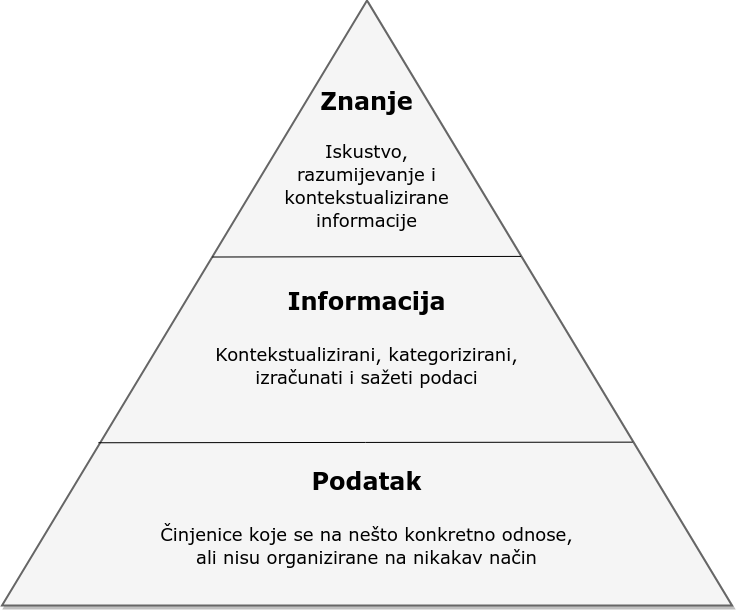
\includegraphics[width=0.75\textwidth]{slike/znanjeinfopodatak.png}
    \caption{Odnos podatka, informacije i znanja \cite{diwdiagram}}
    \label{znanjeinfopodatak}
\end{figure}

\section{Vrste podataka}

Prema obliku u kojem pohranjujemo podatke, možemo ih podijeliti u tri kategorije: strukturirani, polustrukturirani i nestrukturirani podaci. Važno je znati oblik podatka kojeg pohranjujemo kako bi znali koja baza podataka je potrebna za pohranu podataka. \cite{dataEngineerStudyGuide}  U nastavku ovoga poglavlja će se objasniti svaka od nabrojanih kategorija.

\subsection{Strukturirani podaci}

Strukturirani podaci su podaci koji imaju određeni strukturu, odnosno podaci se spremaju prema unaprijed definiranoj shemi. Prije nego se podatak kreira, potrebno je dizajnirati bazu podataka i odrediti shemu kako bi se prema njoj mogli zapisivati podaci. Glavni nedostatak ovakvog tipa podataka je loša fleksibilnost u zapisu informacija. Primjerice, kada bi htjeli jednom redu u relaciji pridružiti još jedan atribut morali bi promijeniti shemu i dodati novi stupac. To može biti izrazito neefikasno za tablice koje sadrže više tisuće redova kojima uopće ni ne treba taj atribut. Glavna prednost ovakvog tipa podataka je što, sa vrlo dobrim performansama, lako je moguće raditi strukturirane upite i vršiti spajanja nad podacima. Najlakši je za pretragu i organizaciju jer se sastoji od redova i stupaca u kojima su pohranjeni podaci. Poslovni korisnici ga lako koriste jer ne treba detaljno razumijeti različite vrste podataka i odnose među njima. Ranjivosti su vrlo rijetke zbog toga što su uslijed niza godina istraživanja, razvoja i poboljšanja one eliminirane. Zbog toga je ovakav tip pohranjivanja podataka danas široko korišten. \cite{unstructuredStructuredSemiStructured}

\begin{figure}[h!]
    \centering
    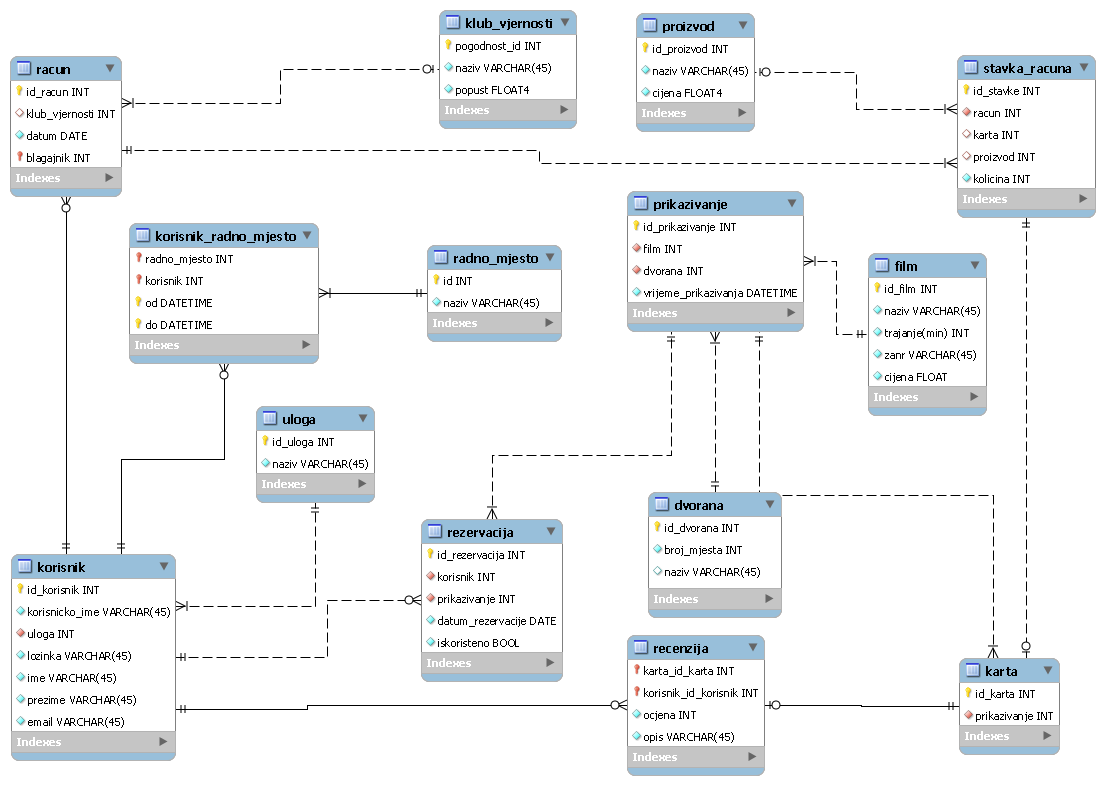
\includegraphics[width=0.95\textwidth]{slike/strukturirani.png}
    \caption{Primjer modela baze koja koristi strukturirane podatke}
    \label{strukturirani}
\end{figure}

Klasičan primjer sustava koji zapisuje strukturirane podatke je relacijska baza podataka. Podaci se nalaze strukturirani u relacijama, odnosno tablicama od kojih se baza podataka sastoji. Relacijska shema baze podataka se sastoji od naziva relacija i popisa atributa. Relacija ili tablica se sastoji od redaka i stupaca (atributa). Atribut, odnosno skup atributa čijim se podacima može jednoznačno identificirati svaki redak naziva se primarnim ključem. \cite{informacijskaTehnologijauPoslovanju} Na slici \ref{strukturirani} je prikazan primjer modela relacijske baze podataka koja koristi strukturirane podatke. Na slici je prikazan ERA model baze podataka za aplikaciju koja je podrška u poslovanju kina. Baza se sastoji od 14 relacija u kojima se podaci spremaju strukturirano prema zadanim atributima.

\subsection{Nestrukturirani podaci}

Nestrukturirani podaci su podaci koji nemaju određenu strukturu, odnosno nije ih moguće spremiti u obliku redova i stupaca u relacijskim bazama. Čine najveći udio od svih podataka u svijetu. Primjer nestrukturiranih podataka su: binarni podaci, tekstualne datoteke, video datoteke, slikovne datoteke i slično. Njihova glavna prednost je što ih nije potrebno klasificirati, ali to ponekada može biti problem u upravljanju sa njima. Kako bi se iskoristili, potrebni su specijalizirani alati i stručnosti u radu sa podacima. Korištenje nestrukturiranih podataka zahtijeva njihovo razumijevanje i razumijevanje kako se podaci mogu povezati kako bi bili korisni. \cite{unstructuredStructuredSemiStructured}

Treba napomenuti da se podaci smatraju nestrukturiranim ako nemaju shemu koja utječe na to kako se podaci pohranjuju ili im pristupaju. Nestrukturirani podaci mogu imati strukturu koja nije relevantna za način pohrane. Na primjer, prirodni jezik je visoko strukturiran prema sintaksičkim pravilima jezika. Audio i video datoteke mogu imati unutarnji format koji uključuje metapodatke kao i sadržaj. Ovdje postoji struktura unutar datoteke, ali sustavi za pohranu ne koriste tu strukturu i to je razlog zašto ova vrsta podataka se klasificira kao nestrukturirana. \cite{dataEngineerStudyGuide} 

\subsection{Polustruktirani podaci}

Polustrukturirani podaci ne zahtijevaju strukturu i predefiniranu shemu što ne znači da ona nije moguća, već je samo opcionalna. Drugi podaci će i dalje neometano postojati ako se shema promijeni ili ako se unese podatak sa novim atributima ili tipom podatka. Podaci se ne mogu pohraniti u obliku redaka i stupaca kao kod strukturiranih podataka. Polustrukturirani podaci sadrže oznake i elemente (metapodatke) koji se mogu koristiti za grupiranje podataka i opisivanje kako se pohranjuju. Na taj način se slični entiteti grupiraju i organiziraju u hijerarhiji. Entiteti u istoj grupi mogu ili ne moraju imati iste atribute i svojstva. Veličina i vrsta istih atributa u grupi se može razlikovati.

Najveća prednost polustrukturiranih podataka je laka prilagodba promjenama u strukturi i fleksibilnost u pogledu razmjene podataka. Podaci su prenosivi i nisu ograničeni fiksnom shemom. Nedostaci su to što je relativno nova tehnologija i zbog toga ovakav tip pohranjivanja podataka nije pretjerano raširen \cite{unstructuredStructuredSemiStructured}. Podaci zbog nepravilne i djelomične strukture mogu otežavati interpretaciju odnosa između podataka. Razlika između sheme i podataka je vrlo nejasna što komplicira oblikovanje strukture podataka. Postoji i izrazita neefikasnost u izvršavanju upita u usporedbi sa strukturiranim modelima podataka zbog specifične strukture zapisa podataka. Još jedan nedostatak je što je i cijena skladištenja viša u odnosu na strukturirane podatke. \cite{tbpknjiga}

Najpoznatiji modeli podataka koji koriste polustrukturirane podatke su Extensible Markup Language (XML) i JavaScript Object Notation (JSON). XML omogućava definiranje XML sheme koju mogu obraditi programi bez smanjenja njihove upotrebljivosti za ljudske čitatelje. Omogućuje korisniku definiranje oznaka i atributa za pohranjivanje u hijerarhijskom obliku. JSON je standardni format koji koristi ljudski čitljiv tekst za prijenos podatkovnih objekata koje se sastoji od parova atribut i vrijednost. Koristi se prvenstveno za prijenos podataka između poslužitelja i mrežnih aplikacija kao alternativa XML-u. JSON i XML upravo najviše koriste web servisi. \cite{cros} U nastavku slijedi primjer JSON podatka:

\begin{lstlisting}
{
   "rezervacija": {
      "broj": 43,
      "timestamp": "2020-07-21T14:26:59.125",
      "potvrdjeno": true
   },
   "vlak": {
      "datum": "25/07/2020",
      "vrijeme": "09:30",
      "od": "Rijeka",
      "do": "Zagreb",
      "sjedalo": "54A"
   }
   "putnik": {
      "name": "Ivan Horvat",
      "status": "Umirovljenik",
   },
   "cijena": 60
}
\end{lstlisting}

Može se vidjeti kako u ovom tipu podatka postoji određena struktura, ali ona nije toliko striktna kao kod strukturiranih podataka. Konkretno kod JSON-a je važno da svaka vrijednost ima svoj naziv, da se podaci razdvajaju zarezom i da vitičaste zagrade moraju sadržavati jedan objekt. Tipovi podataka koje može poprimiti neka vrijednost su: tekst, broj, logička vrijednost, null,  polje ili drugi objekt. 

Za ovaj primjer jedne rezervacije karte za vlak se jasno vidi da ovaj objekt ima četiri vrijednosti:

\begin{itemize}
\item "rezervacija" - tip je objekt koji u sebi sadrži podatke o rezervaciji: broj rezervacije, datum i vrijeme obavljene rezervacije u tekstualnom formatu i logička vrijednost potvrda rezervacije.
\item "vlak" - tip je objekt koji u sebi sadrži podatke o vožnji vlaka: datum polaska, vrijeme polaska, polazište, ishodište i naziv sjedala. Svi podaci su u tekstualnom formatu.
\item "putnik" - tip je objekt koji u sebi sadrži podatke o putniku: ime i prezime i njegov status.
\item "cijena" -  cijena karte u brojčanom formatu
\end{itemize}

\chapter{XML}

XML je primjer zapisa polustrukturiranih podataka koji se koristi za prikaz i razmjenu podataka preko Interneta. Najčešće se koristi još i kao baza podataka, zapisivanje metapodataka, upravljanje informacija i e-commerce. 

XML dokument ima tri komponente: opcionalni prolog, obavezni korijenski element i neobavezni epilog koji dolaze poslije korijenskog dokumenta. Prolog sadrži XML deklaracije i reference na vanjski dokument za strukturiranje. Korijenski element je tijelo XML dokumenta i sadrži elemente i atribute. Ispod njega se može nalaziti epilog koji govore o tome kako treba postupati sa dokumentom. \cite{xmlDatabase}

\begin{figure}[h!]
    \centering
    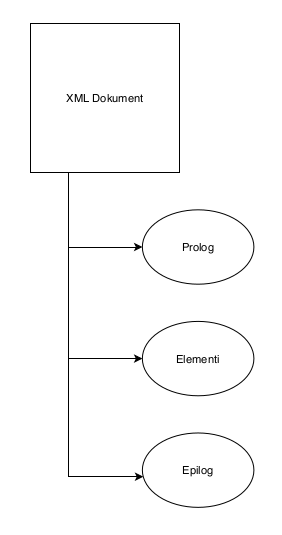
\includegraphics[width=0.4\textwidth]{slike/XMLkomponente.png}
    \caption{Komponente XML dokumenta}
\end{figure}

Sintaksa XML-a je prilično jednostavna i sadrži samo nekoliko jednostavnih pravila koje treba slijediti. XML dokument može biti dobro oblikovan ili valjan. Dobro oblikovan dokument pridržava se brojnih ograničenja dobrog oblikovanja koja su detaljno opisana u XML specifikaciji. XML dokument je valjan ako prema XML specifikaciji ima pridruženu deklaraciju vrste dokumenta i ako je dokument u skladu s ograničenjima izraženima u njoj. Dobro oblikovan XML dokument započinje XML deklaracijom koja mora biti na početku dokumenta i može izgledati ovako:

\begin{lstlisting}[language=XML]
<?xml version="1.0" encoding="EBCDIC" standalone="no" ?>
\end{lstlisting}

Postoje 2 verzije XML-a: 1.0 i 1.1. Prva XML verzija je kreirana 1998. godine., te i dalje je prihvaćena i preporučuje se za korištenje. Bazirana je na filozofiji da je zabranjeno sve što nije dozvoljeno. Druga verzija XML 1.1 je objavljena 2004. godine i sadrži svojstva koja olakšavaju rad sa programima na jačim računalima. Njezin pristup je da je dozvoljeno sve što nije zabranjeno. Potreba za novom verzijom XML-a se javila zbog razvoja drugih standarda na koje se XML oslanja. Prvenstveno je bio problem sa novim Unicode znakovima koje do tada XML 1.0 nije podržavao. Sa novom verzijom se omogućuje korištenje svih budućih Unicode znakova koji će se bilo kada u budućnosti definirati. U XML deklaraciji je potrebno u navodnicima navesti verziju (1.0 ili 1.1) u kojoj je dokument napisan. Nakon deklaracije verzije slijedi deklaracija kodiranja koja označava skup znakova koji se koristi za stvaranje dokumenta. Kao zadano, XML dokumenti kodirani su u Unicode-u, bilo 8-bitnom (UTF-8) ili 16-bitnom (UTF-16). Atribut kodiranja je neobavezan ako se koristi bilo koji od ovih kodiranja, ali se smatra dobrom praksom navesti je.  Atribut "standalone" obavještava XML parser o tome oslanja li se dokument na podatke iz vanjskog izvora kao što je npr. DTD (document type definition). Zadana vrijednost je "no", a ako se postavi na "yes" XML parseru se poručuje da nema dokumenata sa vanjskih izvora.

XML dokument se sastoji od teksta (samih podataka) i oznaka (koje označavaju strukturu dokumenta u aplikaciji koja dokument obrađuje). Oznaka je konstrukcija koja sadržaje dokumenta odvaja lijevim i desnim kutnim zagradama (<>). Parovi oznaka koriste se za ograničavanje podataka. Element je podatkovni objekt kojeg je potrebno identificirati. Naziv elementa je obično opisno ime za podatkovni objekt kojeg element predstavlja. Svaki element u XML dokumentu mora početi s početnom oznakom i završiti sa komplementarnom završnom oznakom. Završna oznaka izgleda kao početna oznaka, osim što završna oznaka uključuje kosu crtu "/" prije naziva elementa. Podaci između početne i završne oznake su sadržaj elementa. Sadržaj može biti tekst ili čak i drugi element sa svojom vlastitom oznakom. U nastavku je prikazan primjer zadavanja elementa:

\begin{lstlisting}[language=XML]
<element> information </element>
\end{lstlisting}

Početna oznaka je <element>. Sadržaj je "information" Završna oznaka je </element>. Sva tri dijela zajedno čine element. Nazivi elemenata moraju početi slovom ili podvlakom. Nakon prvog znaka slijedi nula ili više slova, brojeva, podvlaka ili crtica. \cite{xmlSoapProgramming} U nastavku je prikazan primjer kako bismo zapisali informacije o nekoj osobi:

\begin{lstlisting}[language=XML]
<label>
<name> Jane Smith </name>
<address>
   <street> 270 Burlington Road </street>
   <city> Bedford </city>
   <state> MA 01730 </state>
</address>
</label>
\end{lstlisting}

U ovom primjeru može se vidjeti kako je informacija o nekoj osobi zapisana u elementu  "label" koji sadrži oznaku "name" gdje je opisano ime osobe, te element "address" koji sadrži tri ugniježđena elementa: "street" koji opisuje ulicu, "city" koji opisuje grad i "state" koji opisuje državu. Kod ugniježđenih elemenata je važno da dobro formirani dokumenti ima pravilnu strukturu stabla. Ona se postiže na način da završna oznaka elementa koja se nalazi unutar drugog elementa mora doći prije završne oznake roditelja.

U primjeru su korištene oznake za prikaz informacija. Umjesto oznaka i atributi mogu prikazivati informacije. Ponekad samo imenovanje elemenata nije dovoljno, pa atributi mogu pomoći sa dodatnim opisivanjem. Znak jednakosti razdvaja atribut od njegove vrijednosti i može i ne mora sadržavati razmak s jedne ili obje strane vrijednosti. Vrijednost atributa se obavezno mora navesti unutar navodnika, bilo jednostrukih ili dvostrukih. Ako vrijednost atributa mora sadržavati navodnike, moguće je vrijednost atributa navesti sa jednom vrstom navodnika, a podatak unutar atributa sa drugom vrstom. Iznimno, ako je potrebno imati istu vrstu navodnika u oba slučaja to se može postići sa specijalnim znakovima. Atribut se ne smije staviti na završnu oznaku elementa. Stoga prema objašnjenim pravilima, element "address" iz prošlog primjera može se prikazati kao element koji sadrži atribute "street", "city" i "state": \cite{xmlDatabase}

\begin{lstlisting}[language=XML]
<address
street = “270 Burlington Road”
city = “Bedford”
state = “MA 01730”
/>
\end{lstlisting}

XML dokument mora imati jedinstveni korijenski element: element koji ima početnu oznaku na vrhu dokumenta, a krajnju oznaku na dnu dokumenta. Prva početna oznaka koja se napiše u dokumentu smatra se korijenskim elementom. Čim se nađe krajnja oznaka za element, dokument je završio. Nakon završetka korijenskog elementa ne smije se započeti sa pisanjem nekog drugog elementa jer je samo jedan element dopušten na razini korijena.

Svi XML elementi i nazivi atributa su osjetljivi na veliko i malo slovo, što znači da ako se element započne sa oznakom <element>, on se mora završiti sa oznakom </element>. Ispravan završetak elementa neće biti oznaka </ELEMENT>, </Element> ili neki drugi oblik jer je važno poštivati veliko/malo slovo. U XML-u je moguće zadati i prazne elemente koji se razlikuju od običnih elemenata u tome što nemaju nikakav sadržaj. Oznaka praznog elementa počinje sa nazivom oznake, a završava sa znakovima "/>" koji moraju biti zajedno napisani bez razmaka. Prazan element može imati i atribute kao i običan element. U XML-u je moguće pisati i komentare koji mogu davati neke korisne informacije o dokumentu. Početak komentara se označava sa znakovima "<!--", a komentar završava sa znakovima "-->". Unutar komentara može se proizvoljno pisati jer će XML parser ignorirati sve unutar navedenih znakova. \cite{xmlSoapProgramming}

Ako netko želi stvoriti svoj jezik temeljen na XML-u može to učiniti na način da sam kreira sve oznake ili da kreira jedan dio oznaka, a ostale uzme iz nečijeg XML dokumenta. Kako bi se razlikovali elementi uzeti od tuđeg XML dokumenta stvoren je mehanizam dodijele jedinstvenih imena strukturama dokumenta, a naziva se XML Namespaces. Oni omogućavaju pridjeljivanje konteksta elementima, što omogućuje elementima da budu jedinstveni. Imenik je obavezno deklarirati u dokumentu prije nego se koristi.

\section{XPath}

XPath (XML Path Language) je upitni jezik za odabir čvorova iz XML dokumenta. Zasnovan je na stablastoj strukturi XML dokumenta i omogućuje kretanje po stablu odabirom čvorova prema raznim kriterijima. Stvoren je od strane World Wide Web Consortium (W3C), iste grupacije koja je kreirala XML i standardizirani HTML. U uporabi je nekoliko verzija XPath-a: XPath 1.0 (objavljen 1999. godine i još uvijek najkorištenija verzija), XPath 2.0 (objavljen 2007. godine  i omogućuje veći izbor tipova sustava), XPath 3.0 (objavljen 2014. godine i omogućuje implementaciju funkcija) i XPath 3.1. (objavljen 2017. godine i omogućuje nove tipove podataka i bolju podršku za JSON).

Svaki XPath se piše u obliku: "axis :: node-test [predicate]*" gdje axis predstavlja smjer navigacije unutar stabla XML dokumenta, node-test predstavlja putanju čvorova, a predikati (koji se nalaze u uglatim zagradama) služe za filtriranje čvorova prema određenom uvjetu. Kako bi se moglo raditi sa podacima u XML dokumentu, XPath omogućuje nekoliko tipova podataka koje se mogu proslijediti u XPath izraz:
\begin{itemize}
\item Brojčani tip podatka - u XPath izraz se može proslijediti broj, npr. izraz "//planet[position()=7]" će vratiti sedmi element <planet> u XML dokumentu. Postoje i brojčani operatori preko kojih se može dobiti brojčana vrijednost: +, -, *, div i mod. Postoji i nekoliko funkcija koje izraz vraćaju u brojčanu vrijednost: funkcija "ceiling" zaokružuje broj na prvi veći cijeli broj, funkcija "floor" zaokružuje broj na prvi manji cijelu broj, funkcija "round" zaokružuje broj na najbliži cijeli broj i funkcija "sum" vraća zbroj proslijeđenih brojeva.
\item Tekstualni izraz - u XPath izraz se može proslijediti niz od nula ili više znakova gdje su znakovi prema zadanom u Unicode formatu, npr. izraz "//planet[name="Mars"]" će vratiti sve elemente <planet> koji imaju dijete <name> čija je tekstualna vrijednost jednaka "Mars". Postoji i nekoliko funkcija preko kojih se može manipulirati sa tekstualnim izrazom: funkcija "concat" spaja sve proslijeđene tekstualne izraze, funkcija "contains" vraća istinitu logičku vrijednost ako je tekstualni izraz jednak onome proslijeđenom, funkcija "normalize-space" briše razmake na početku i kraju izraza i pretvara više razmaka unutar izraza u jedan razmak, funkcija "starts-with" vraća istinitu logičku vrijednost ako tekstualni izraz započinje sa proslijeđenim izrazom, funkcija "string-length" vraća broj znakova u izrazu, funkcija "substring" vraća podniz nekog izraza, funkcija "substring-after" vraća podniz nakon proslijeđenog izraza, funkcija "substring-before" vraća podniz prije proslijeđenog izraza i funkcija "translate" vraća izraz sa svim pojavama znakova u drugom izrazu zamijenjenom odgovarajućim znakovima u trećem tekstualnom izrazu.
\item Logička vrijednost - XPath izraz može biti logička vrijednost true/false, npr. izraz "position()=3" će vratiti true ako je pozicija jednaka trećem čvoru u elementu ili će vratiti false ako tvrdnja ne vrijedi.  Logičkih operatori preko kojih se može dobiti logička vrijednost su: !=, <, > i >=. Postoji i nekoliko funkcija koje izraz vraćaju u logičku vrijednost: funkcija "boolean" pretvara argument u logičku vrijednost, funkcija "false" vraća lažnu vrijednost, funkcija "true" vraća istinitu vrijednost, funkcija "lang" ispituje je li jezik čvora isti jeziku proslijeđenom u funkciju, funkcija "not" mijenja logičku vrijednost njenog argumenta.
\item Set čvorova - XPath izraz može filtrirati čvorove na način da vrati set od nula ili više čvorova prema zadanom izrazu, npr. izraz "//planet[position() > 3]" će vratiti sve elemente <planet> nakon prva tri elementa. Postoje i funkcije koje mogu raditi nad setom čvorova. Funkcija "position" vraća broj koji predstavlja poziciju čvoru u sekvenci čvorova koje se obrađuju i funkcija "count" vraća broj čvorova u danom setu čvorova.
\end{itemize}

Axis ili os se piše na početku XPath izraza i predstavlja smjer navigacije unutar stabla XML dokumenta. Predstavlja vezu između trenutnog čvora sa drugim čvorovima u dokumentu i koristi se za lociranje čvorova u odnosu na taj čvor u stablu. Postoji 13 osi koji se mogu zadavati u XPath izrazu:
\begin{itemize}
\item ancestor : odabire sve pretke (roditelje, roditelje roditelja, itd.) od trenutnog čvora
\item ancestor-or-self : odabire trenutni čvor i sve pretke (roditelje, roditelje roditelja, itd.) od trenutnog čvora
\item attribute : odabire se atribute od trenutnog čvora
\item child : odabire svu djecu od trenutnog čvora
\item descendant : odabire sve potomke (djecu, unuke, itd.) od trenutnog čvora
\item descendant-or-self : odabire trenutni čvor i sve potomke (djecu, unuke, itd.) od trenutnog čvora
\item following : odabire sve u XML dokumentu nakon završne oznake od trenutnog čvora
\item following-sibling : odabire svu braću od trenutnog čvora
\item namespace : odabire sve čvorove prostora imena trenutnog čvora
\item parent : odabire roditelja trenutnog čvora
\item preceding : odabire sve čvorove koji se pojavljuju prije trenutnog čvora u dokumentu osim predaka i čvorova prostora imena
\item preceding-sibling : odabire svu braću koji se pojavljuju prije trenutnog čvora
\item self : odabire trenutni čvor
\end{itemize}

XPath koristi izraze puta za odabir čvorova u XML dokumentu. Čvor se bira slijedeći putanju ili korake. Sve čvorove sa određenim imenom može se odabrati tako da se upiše naziv tog čvora. Odabir korijenskog čvora se postiže sa izrazom "/". Odabir svih čvorova koji odgovaraju selekciji gdje god u dokumentu oni bili se postiže sa izrazom "//". Trenutni čvor se može odabrati sa izrazom ".", a roditelja trenutnog čvora se odabire sa "..". Atributi u čvoru se mogu odabrati sa izrazom "@". Bilo koji element čvora se označava sa oznakom "*", bilo koji atribut čvora se označava sa oznakom "@*", a bilo koji čvor bilo koje vrste se dobije sa izrazom "node()". Korištenjem "|" operatora u izrazu XPath može se odabrati nekoliko različitih staza. \cite{XPath}

\section{XQuery}

XQuery je funkcionalan upitni jezik koji se koristi za pronalaženje podataka pohranjenih u XML formatu. Smatra se da je XQuery za XML isto ono što je SQL za relacijsku bazu podataka. Dizajniran je za pronalaženje i vraćanje elemenata i atributa iz XML dokumenta, a izgrađen je na XPath izrazima koje koristi za kretanje kroz XML dokument. Može se koristiti još za izdvajanje podataka web servisu, generiranje sažetka izvještaja, pretvorbu XML podataka u XHTML dokument i pretragu Web dokumenta. Općenito se može koristiti za dohvaćanje hijerarhijskih i tabličnih podataka, te za ispitivanje stabla i grafičkih struktura. Najbolji je za baze podataka temeljene na XML-u i objektne baze podataka. Stvoren je od strane World Wide Web Consortium (W3C) 2007. godine, a najnovija verzija XQuery 3.1 je W3C preporuka od 21. ožujka 2017. godine.

Elementi, atributi i varijable koje se koriste u XQuery moraju biti valjani XML nazivi u dokumentu. Važno je i obratiti pozornost na velika i mala slova jer XQuery je osjetljiv na tu razliku. Varijabla je definirana sa oznakom "\textdollar " praćena nazivom varijable, npr. "\textdollar bookstore". Tekstualni izraz mora biti unutar jednostrukih ili dvostrukih navodnika. Komentari se navode tako da se početak označi sa "(:", a kraj sa ":)". Upiti se tvore pomoću izraza FLWOR nastalih po prvim slovima klauzula koje se koriste:

\begin{itemize}
\item \textbf{F}or - koristi se za označavanje čvora
\item \textbf{L}et - koristi se za postavljanje vrijednosti varijable
\item \textbf{W}here - koristi se za filtriranje čvorova
\item \textbf{O}rder by - koristi se za sortiranje čvorova
\item \textbf{R}eturn - koristi se za određivanje odgovora koji će se vratiti
\end{itemize}

U jednom XQuery izrazu moguće je koristiti više upita sa ključnim riječima for i let, a obavezan je barem jedan izraz sa klauzulom for ili let. Klauzule where i order by su opcionalne prilikom korištenja klauzule for. Na kraju je obavezna klauzula return koja određuje izraz koji se vraća kao odgovor. Slično kao i kod XPath-a, ovdje se prema XML dokumentu odnosi kao prema stablu sa čvorovima gdje je korijen stabla korijenski čvor i njemu se pristupa preko funkcije doc().

XQuery, XPath i XSLT dijele istu biblioteku funkcija. Postoji još nekoliko vrsta funkcija koje nudi XQuery za rad sa podacima  \cite{javatpoint}:
\begin{itemize}
\item Funkcije pristupa - node-name (vraća naziv čvora), nilled (vraća true ako je čvor u argumentu nil, odnosno ne sadrži ništa), data (vraća atomarnu vrijednost čvora), base-uri (vraća svojstvo base-uri od trenutnog ili određenog čvora), document-uri (vraća svojstvo document-uri od određenog čvora)
\item Funkcije pogrešaka i praćenja - error (ispisuje grešku), trace (za otklanjanje neispravnosti upita)
\item Numeričke funkcije - abs (vraća apsolutnu vrijednost broja), ceiling (zaokružuje broj na prvi veći cijeli broj), floor (zaokružuje broj na prvi manji cijeli broj), round (zaokružuje broj na najbliži cijeli broj)
\item Tekstualne funkcije - string-length (vraća duljinu teksta), concat (spaja tekstove zadane u argumentu u jedinstveni tekstualni izraz), string-join (spaja tekstove zadane u argumentu sa zadnim delimiterom u jedinstveni tekstualni izraz)
\item Logičke funkcije - boolean (vraća logičku vrijednost argumenta), not (negacija logičke vrijednosti), true (vraća istinitu logičku vrijednost), false (vraća lažnu logičku vrijednost)
\item Vremenske funkcije - current-date (vraća trenutni datum), current-time (vraća trenutno vrijeme), current-datetime (vraća trenutni datum i vrijeme)
\item Funkcije čvora - node-kind (provjerava je li argument proslijeđen u funkciju čvor), node-name (vraća prošireni QName naziv čvora proslijeđenog kao argument), local-name (vraća lokalni naziv proslijeđenog čvora)
\item Funkcije sekvence - count (daje broj elemenata u sekvenci), sum (zbraja elemente iz sekvenci), avg (računa prosječnu vrijednost elemenata u sekvenci), min (vraća najmanju vrijednost iz sekvence), max (vraća najveću vrijednost iz sekvence), distinct-values (vraća sekvencu bez dupliciranih elemenata), subsequence (vraća podniz iz dobivenog niza), insert-before (unosi element u sekvencu), remove (briše element iz sekvence), reverse (vraća preokrenutu sekvencu), index-of (vraća indeks nekog elementa iz sekvence), last (vraća zadnji element iz sekvence), position (vraća broj koji predstavlja poziciju čvora u sekvenci čvora koji se obrađuje)
\item Kontekstualne funkcije - omogućuju kreiranje novog konteksta upita, upravljati sa trenutnim kontekstom ili dohvatiti informacije o trenutačnom kontekstu
\end{itemize}

Od verzije 3.0, XQuery nudi dodatne korisne značajke. Kako bi se omogućio rad sa najnovijom verzijom XQuery, potrebno je upit započeti sa naredbom "xquery version 3.1;". Nova verzija donosi try/catch mehanizam kako bi se mogle uhvatiti eventualne greške prilikom izvršavanja upita, switch izraz koji omogućuje izvršavanje samo jednog dijela koda, funkcije, jednostavniji operatori mapiranja, jednostavnije spajanja tekstualnih izraza pomoću operatora "||", anotacije za funkcije i varijable koje se mogu odrediti kao privatne ili javne. Možda najzanimljivija novost koja je došla od verzije 3.0 je dodavanje Group by klauzule u FLWOR izraz koji time omogućuje grupiranje podataka dobivenih prilikom upita. \cite{exist}

\chapter{XML baza podataka}

XML baza podataka je sustav za održavanje podataka koji omogućuje njihovu uporabu i pohranjivanje u XML formatu. Postoje dvije vrste XML baza podataka:
\begin{itemize}
\item XML-enabled baze podataka (XED) - ovaj tip baze podataka radi slično kao relacijska baza podataka, odnosno podaci se pohranjuju u tablici u obliku redova i stupaca. Obično su implementirane kao dodatak u drugim sustavima za upravljanje bazom podataka gdje je moguće preslikavanje XML dokumenta u određenu bazu. Podaci koji se pritom preslikavaju mogu izgubiti metapodatke i strukturu zadanu u dokumentu. Najpoznatije realizacije XML-enabled baze podataka su: Oracle 9i, Oracle 10g, Microsoft SQL Server, IBM DB2 itd.
\item Native XML baze podataka (NXD) - koristi se za pohranu velike količine podataka i umjesto tabličnog formata on slijedi XML model za pohranjivanje podataka. Ova vrsta baze podataka ima potpunu kontrolu nad XML-om i time je poželjniji jer omogućuje visoku sposobnost pohrane, održavanja i pregledavanja XML dokumenta, te dohvat podataka pomoću XQuery ili XPath izraza.
\end{itemize}

Odlučivanje o vrsti baze podataka koja će se koristiti ovisi o specifičnim zahtjevima aplikacije i formatu XML dokumenta. Potrebno je odrediti je li XML dokument usmjeren na podatke ili na dokument kao cjelinu. XML dokument usmjeren na podatke se koristi prilikom interoperabilnosti, te ima čvrstu strukturu, sitnozrnate podatke i ne sadrži miješani sadržaj. Za rad sa njima preporučuje se XML-enabled baze podataka. XML dokumenti usmjereni na dokument kao cjelinu su uglavnom izrađeni za ljude, te nemaju čvrstu strukturu i imaju grubo-zrnate podatke do te mjere da najmanja neovisna podatkovna jedinica može biti cijeli dokument. Ključni elementi ovog tipa XML dokumenta su polustrukturirani podaci, te za rad sa njima se preporučuju Native XML baze podataka. \cite{xmlDatabase} Zbog specifičnosti aplikacijske domene objašnjene u idućem poglavlju, za potrebe ovoga rada koristit će se Native XML baza podataka, sustav eXist-db. Ostale popularne realizacije NXD baze podataka su: BaseX, Sedna, 28.io, MarkLogic Server.

BaseX je lightweight sustav za NXD bazu podataka sa dodatnim aplikacijskim poslužiteljima napisanim na Javi. Objavljen je kao open-source aplikacija 2007. godine. BaseX omogućava jednostavno GUI sučelje za korištenje napisano u programskom jeziku Java. U odnosu na eXist, BaseX postiže 99,9\% usklađenosti s W3C XQuery 1.0 specifikacijom (eXist ima 99,4\%) i implementira specifikacije za XQuery Update 1.0 i XQuery Full-Text. eXist ima stariju verziju implementacije XQuery Update, ali je dostupan dulje od BaseX pa podržava mnoge druge značajke, poput XSLT-a.

Sedna je lightweight sustav za NXD bazu podataka napisan u programskim jezicima C i C++. Podrijetlo Sedne nije dobro dokumentirano, ali čini se da je započelo oko 2003. kao projekt Instituta za sistemsko programiranje Ruske akademije znanosti. U usporedbi s eXistom, Sedna izravno podržava više API-ja za različite programske jezike. Iako nema vlastiti REST poslužitelj, može se konfigurirati da radi kao modul unutar Apache HTTP poslužitelja. Sedna postiže 98,8\% usklađenosti s W3C XQuery 1.0 specifikacijom što je manje od onoga što postiže eXist.

28.io je PaaS (platforma kao usluga) za Zorba open source i integrira Zorbu s MongoDB, podupirući pohranu i indeksiranje XML-a u MongoDB kao glavnu bazu podataka. U usporedbi s eXistom, 28.io nudi uslugu na oblaku i upravlja svojom bazom podataka u potpunosti koristeći XQuery, dok eXist nudi administrativne GUI alate i dodatne API-je. 28.io, slično kao eXist, omogućava aplikacijsku platformu poslužitelja koja omogućuje izgradnju čitavih aplikacija pomoću XQueryja. 28.io (preko Zorba) ima sličnu kompatibilnost s W3C XQuery 1.0 specifikacijom kao eXist, te također podržava XQuery Update, XQuery Full-Text i XQuery Scripting. 28.io je razvila 28msec, tvrtka sa sjedištem u Zürichu u Švicarskoj.

MarkLogic Server je sustav za NXD bazu podataka napisan u C++ koji omogućuje rad sa XQuery upitima i XSLT transformacijom podataka. Razvila ga je MarkLogic Corporation iz SAD, Kalifornije. MarkLogic nudi mogućnost upravljanja velikim količinama podataka (više od petabajt XML podataka), dok eXist može raditi puno skromnije (nekoliko stotina gigabajta, ali to uvelike ovisi o skupu podataka i upitima). Najveća prednost MarkLogica što u odnosu na druge slične sustave ima bolje skaliranje velikog skupa podataka. \cite{exist}

\section{eXist-db}

eXist-db (ili skraćeno eXist) je besplatan i otvoreni sustav za native XML bazu podataka (NXD) napisan u programskom jeziku Java. Kreiran je 2000. godine, a trenutna verzija (5.0) izašla je u rujnu 2019. godine. Dobitnik je nagrade za najboljeg pružatelja XML baze podataka 2006. godine od strane InfoWorld-a. Baza podataka je sastavljena od XML dokumenata povezanih u direktorije koje se zovu kolekcije. Glavna prednost eXist-a u odnosu na druge NoSQL sustave je mogućnost korištenja standardiziranog XQuery upitnog jezika za rad sa dokumentima. eXist-db osim XQuery-a omogućava i još neke dodatne standarde i tehnologije: XPath, XSLT, XSL-FO, WebDAV, REST, RESTXQ, XInclude, XML-RPC, XProc. \cite{exist-definition}

eXist se može instalirati na gotovo svim verzijama operacijskih sustava Linux, Windows i Mac OS X. Najvažniji faktor je da operacijski sustav ima predinstaliran JRE (Java Runtime Environment) ili JDK (Java Delevopment Kit) verzije 1.6 ili novije. Proces instalacije je jednostavan: potrebno je sa službene stranice (http://www.exist-db.org) preuzeti željenu verziju i pratiti korake instalacije. eXist prema zadanome koristi dva TCP porta: port 8080 koji služi za običnu HTTP komunikaciju i port 8443 koji služi za sigurnu HTTPS komunikaciju. Nužno je osloboditi ova dva porta kako bi eXist mogao pravilno raditi, a eventualno se u postavkama mogu promijeniti brojevi portova. Poslužitelj se pokreće desnim klikom na ikonu u traci sustava i odabirom opcije "Start server". Moguće je i pokrenuti poslužitelj preko upravljačke konzole tako da se pozicionira u direktorij gdje je eXist instaliran i pozove naredba "java -jar start.jar". Nakon uspješnog pokretanja, preko Web preglednika se može pristupiti upravljačkoj ploči eXista da se kao adresa upiše "http://localhost:8080". Kako bi se bez ograničenja mogle koristiti sve opcije potrebno se prijaviti sa korisničkim imenom i lozinkom zadanom prilikom instalacije. Na slici \ref{exist-dashboard} je prikazan izgled upravljačke ploče programa eXist.

\begin{figure}[h!]
    \centering
    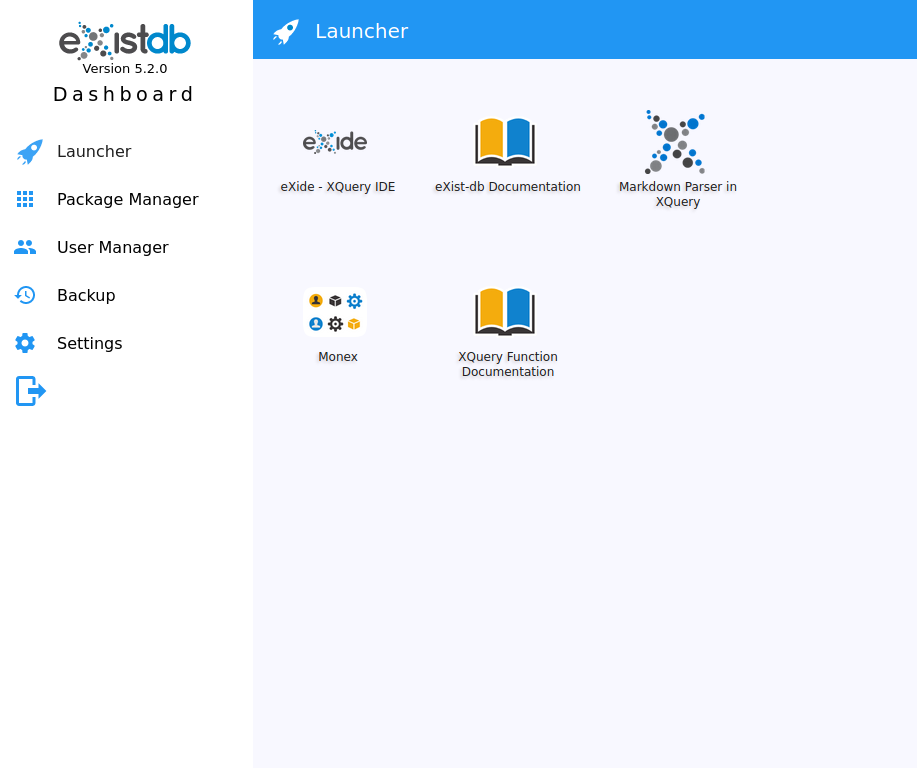
\includegraphics[width=1\textwidth]{slike/exist-dashboard.png}
    \caption{eXist upravljačka ploča}
    \label{exist-dashboard}
\end{figure}

U upravljačkoj ploči moguće je odabrati nekoliko alata i dodatnih paketa koje će u nastavku biti objašnjene. eXide je razvojno okruženje koje može raditi sa XQuery, XML i ostalim resursima pohranjenim u eXide. Sa njim je moguće kreirati nove dokumente ili održavati postojeće. Podržava nekoliko mogućnosti koje postoje u popularnim i modernim razvojnim okruženjima poput refaktoriranja, automatskog nadopunjavanja i slično. eXist-db Documentation omogućava pristup dokumentaciji koja opisuje i olakšava rad sa programom. Pomoć u radu mogu pružiti i opcije Markdown Parser in XQuery i XQuery Function Documentation koji mogu olakšati shvaćanje rada sa XQuery-em. U upravljačkoj ploči je moguće odabrati opciju Monex koja prikazuje statistiku rada sa bazom podataka. U realnom vremenu je moguće promatrati zauzeće resursa na bazi, pratiti rad upita i indeksa, povezati bazu na udaljeni poslužitelj, omogućiti rad sa bazom na tom poslužitelju i slično. S lijeve strane upravljače ploče pod izbornikom Package Manager moguće je upravljati, instalirati i deinstalirati dodatne pakete. Izbornik User Manager omogućava dodavanje i brisanje korisnika i grupa korisnika. Pod izbornikom Backups moguće je napraviti sigurnosnu pohranu ili odrediti vremenske intervale kada bi se ta sigurnosna pohrana događala. Pod izbornikom Settings moguće je izmijeniti postavke programa. Zadnja mogućnost u izborniku s lijeve strane odjavljuje trenutno aktivnog korisnika iz upravljačke ploče.

Java Admin Client je jednostavna kontrolna aplikacija eXist-a kojoj se može pristupiti odabirom opcije na ikoni u traci sustava. Aplikacija omogućava rad sa bazom podataka, kreiranje novih kolekcija, kreiranje i vraćanje sigurnosnih pohrana, izvoz i uvoz podataka, postavljanje baze podataka i slično. Na slici \ref{javaAdminClient} prikazan je izgled navedene aplikacije. Nakon uspješne autorizacije korisniku se prikazuje popis kolekcija u bazi podataka. Korijenska kolekcija u bazi podataka je "/db" i njen naziv nije moguće promijeniti. U njoj je moguće dodavati vlastite kolekcije po želji kao što je za potrebe ovog diplomskog rada izrađena kolekcija "diskuto". Prema zadanome u korijenskoj kolekciji postoje još neke važne kolekcije poput "/db/system" gdje eXist sprema konfiguracijske informacije i "/db/apps/*" gdje se nalaze svi paketi instalirani tijekom instalacije ili ručno poslije.

\begin{figure}[h!]
    \centering
    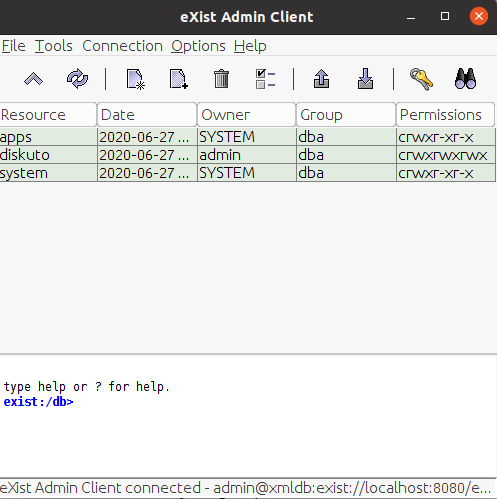
\includegraphics[width=0.85\textwidth]{slike/javaAdminClient.png}
    \caption{Java Admin Client}
    \label{javaAdminClient}
\end{figure}

Mnogo je načina kako se može pristupiti i upravljati sa podacima u eXist-u. Već je objašnjeno kako se to može preko aplikacije Java Admin Client ili razvojnog okruženja eXide, ali osim toga bazi je moguće pristupiti preko  eXist's WebDAV sučelja preko adrese "http://localhost:8080/exist/webdav/db/", preko vanjskih razvojnih okruženja koje imaju opciju za rad sa eXist-om (poput oXygen) ili preko ugrađenih biblioteka za rad sa Ant poslužiteljom na kojem će biti izrađen i projektni dio ovog diplomskog rada.

eXist-db nudi brojne prednosti u odnosu na sustave za upravljanje relacijskim bazama podataka (RDBMS) ili druge NoSQL baze podataka. Zbog korištenja XML-a i orijentacije na dokument, eXist rješava probleme sa kojima se suočavaju drugi sustavi. RDBMS, ali i neke NoSQL baze podataka zahtijevaju da se prema definiranoj shemi zapisuju podaci, dok za eXist ona nije nužna što donosi fleksibilnost u radu sa podacima. eXist koristi XML dokumente za pohranu podataka, dok mnoge druge NoSQL baze (poput MongoDB i Apache Cassandra) umjesto XML, spremaju dokumente u JSON formatu. XML ima znatno više pozitivnih značajki u odnosu na JSON, što je već i objašnjeno u ovom radu, ali jedna od ključnih prednosti XML-a u odnosu na JSON je što omogućuje rad sa kompleksnijim strukturama dokumenta. eXist omogućuje W3C standardizirani upitni i transformacijski jezik XQuery i XSLT, što znači da na svim drugim sustavima koji ih podržavaju oni će raditi identično kao i na eXistu. RDBMS obično koriste također standardizirani SQL upitni jezik, no u praksi neki složeniji upiti neće raditi na različitim proizvodima RDBMS. Sa druge strane, većina NoSQL baza podataka nemaju standardiziran upitni jezik već je on za svaki zasebni proizvod jedinstven. Kao i mnogi drugi sustavi za upravljanje bazom podataka, eXist omogućuje definiranje indeksa za pretragu što, uz orijentiranje na dokument kao cjelinu, dovodi do toga da su rezultati pretrage preciznije od nekih drugih sustava poput TEI, DocBook i DITA. eXist podržava i XForms koji je još jedan W3C standard. Sa njime je moguće korisnički unos jednostavno zabilježiti u XML dokument u bazi podataka. Većina RDBMS i NoSQL baza podataka omogućuju kontroliranje transakcija prema bazi podataka. Nažalost, eXist trenutno ne podržava transakcije na razini baze podataka, ali korištenje baze podataka se sprema u dnevnik baze podataka što osigurava trajnost i konzistenciju podataka. \cite{exist}

\chapter{Opis aplikacijske domene}

Kao praktični dio ovog rada izradit će se XML baza podataka na programskoj platformi eXist-db za potrebe internetskog foruma. Aplikacija koja će koristiti izrađenu bazu podataka će biti realizirana kao Java web-aplikacija. U ovom poglavlju će se definirati internetski forum koji je aplikacijska domena praktičnog dijela rada. Zatim slijedi opis funkcionalnosti izrađene web-aplikacije pod nazivom "Diskuto".

\section{Internetski forum}

Internetski forum je mrežna aplikacija koja omogućava komunikaciju između više ljudi o nekoj određenoj temi. Sudionici na forumu su najčešće anonimni, a eventualno za sudjelovanje u njemu se može zahtijevati registracija korisničkim imenom i lozinkom.  Sve poruke koje korisnik napiše i pošalje su vidljive svim ostalim sudionicima. \cite{definitionInternetForum} Zbog toga se internetski forum ponekad naziva oglasna ploča (eng. discussion board). Poruke se mogu ostavljati i čitati bez ograničenja. Radi lakšeg snalaženja forum je podijeljen u nekoliko kategorija prema temama razgovora. Unutar njih se nalaze objave koje otvaraju i započinju korisnici. Postoji više vrsta korisnika:

\begin{itemize}
\item Neregistrirani korisnici, zovu se još i gosti, nemaju pravo sudjelovati u raspravama, ali zato mogu čitati i pregledavati sadržaj. Poneki forumi striktno zahtijevaju registraciju korisnika kako bi mogao i čitati forum. Postoje korisnici koji su vrlo česti posjetioci foruma, ali ne sudjeluju u njemu već samo pregledavaju objave. U Internet slangu takav korisnik se naziva "lurker", što dolazi od engleske riječi "to lurk" koja znači skrivanje ili vrebanje nekoga ili nečega u zasjedi.\cite{lurker}
\item Registrirani korisnici su obični korisnici koji sudjeluju u raspravama, otvaraju objave, komentiraju i tako pridonose internetskom forumu.
\item Moderatori (kratica "mod") su registrirani korisnici koji imaju prava poput: brisanja, spajanja, premještanja, razdvajanja, zaključavanja ili uređivanja objava. Mogu blokirati, odblokirati, suspendirati ili upozoravati obične korisnike foruma, sve u svrhu boljeg održavanja foruma.
\item Administratori (kratica "admin") su registrirani korisnici koji vode internetski forum. Imaju iste ovlasti kao i moderatori, a uz to mogu promovirati obične korisnike na moderatore, upravljati pravilima, kreirati sekcije, uređivati izgled foruma, te raditi razne operacije nad bazom podataka.\cite{adminvsmoderator}
\end{itemize}

Osim gore opisanog, postoje još neke funkcionalnosti koje su sadržane na većini internetskih foruma. Privatne poruke (kratica "PM" od engleske riječi "private message" za privatnu poruku) služe za slanje privatne poruke od jednog korisnika prema drugom korisniku. Obično se takve poruke koriste za osobnu komunikaciju. Korisnik može prilikom slanja uz poruku učitati i datoteku kao prilog. Datoteka se pritom sprema na poslužitelj od foruma, stoga se moraju definirati ograničenja nad datotekama (tip datoteke i veličina datoteke). Na nekim internetskim forumima korisnik može oblikovati sadržaj svoje poruke koristeći HTML. Kroz internetske forume su popularizirani i emotikoni ili smajlići, odnosno slikovni prikaz korisnikovog raspoloženja ili osjećanja. Korisnik može drugog korisnika staviti na listu ignoriranja čime neće više vidjeti njegove objave. Mnogi forumi omogućuju korisnicima da postave svoj potpis (kratica "sig" od engleske riječi "signature" za potpis) koji postaje vidljiv na kraju svake korisnikove objave. Korisnik se može i pretplatiti na pojedine dijelove foruma, da ne bi propustio sadržaj objavljen sa tog dijela foruma.\cite{vbulletinhelp}

Svaki forum sadrži i popis pravila kojih se korisnici moraju pridržavati. Kršenje pravila sankcioniraju administratori i moderatori, a nepridržavanje pravila mogu prijaviti i obični korisnici. Ako netko prekrši pravilo foruma, prvo ga se obično upozori preko privatne poruke. Ako korisnik nastavlja kršiti pravila zabranjuje mu se pristup forumu na određeni broj dana. Ako i dalje nastavlja kršiti pravila produžuje mu se zabrana pristupa forumu, a može dobiti i trajnu zabranu. Sadržaj koji krši pravila se obično obriše, a ponekad i tema koja je kontroverzna se zaključa i onemogući se korisnicima daljnja rasprava. \cite{rules} Upravo zbog učestalog kršenja pravila Reddit je nedavno trajno uklonio "r/The\_Donald", jednu od najvećih zajednica pristaša američkog predsjednika Donalda Trumpa sa oko 790.000 korisnika. Uklonjeno je stotine tisuća objava i milijuni komentara napisanih od početka djelovanja, 2015. godine. Kao razlog uklanjanja Reddit je naveo poticanje na nasilje i uznemiravanje drugih članova i zajednica Reddit-a. \cite{bannedTheDonald}

\begin{figure}[h!]
    \centering
    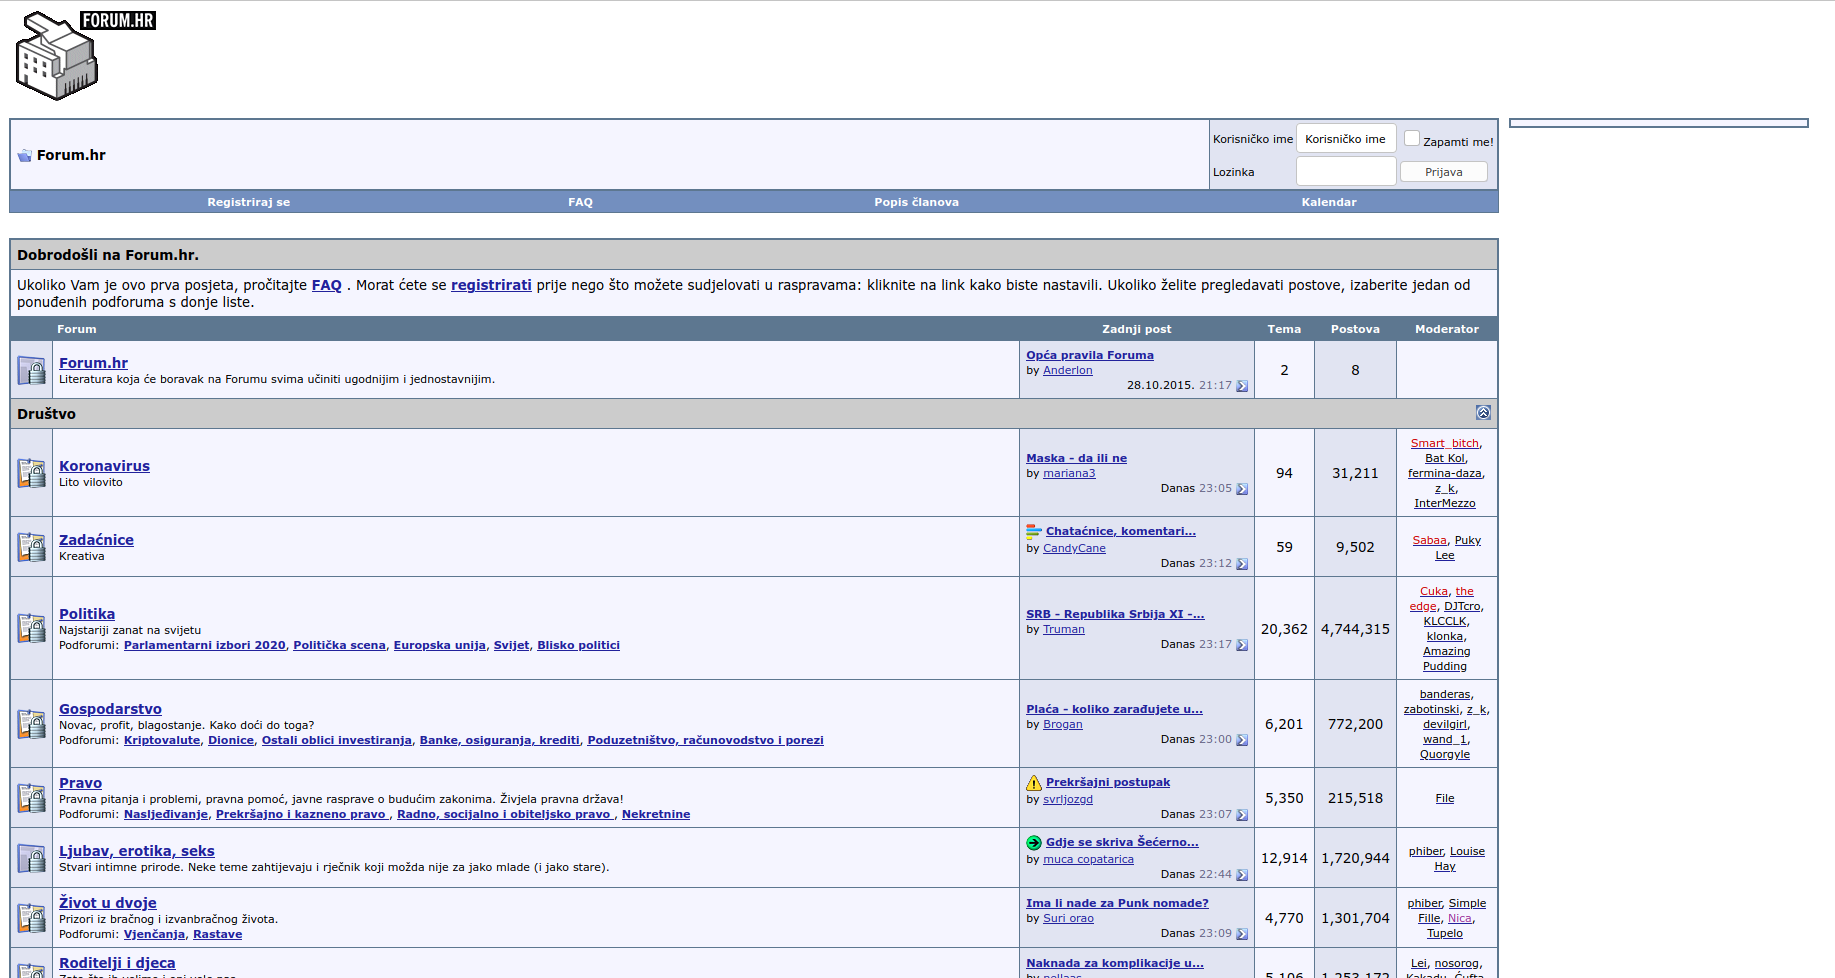
\includegraphics[width=1\textwidth]{slike/forumhr.png}
    \caption{Slika zaslona foruma Forum.hr}
    \label{forumhr}
\end{figure}

Internetski forumi postoje još od samih početaka Interneta. Prve online zajednice i forumi su bili razvijani na BBS (eng. Bulletin Board System) 70-tih godina prošlog stoljeća. Najraniji takvi forumi su bili EIES (eng. Electronic Information Exchange System, nastao 1976. godine) i KOM (šved. KOMpatibila system, nastao 1977. godine). The WELL je najstariji aktivni forum. Razvijen je 1985. godine, ali nije pretjerano popularan jer ima oko 2700 članova. \cite{forumhistory} Neki najpopularniji svjetski forumi su: Reddit, Stack Overflow, Quora, India-Forums, Askubuntu i TripAdvisor. \cite{topforums} U Hrvatskoj je najstariji i najpoznatiji Forum.hr (slika \ref{forumhr}). Razvijen je 1999. godine i sadrži preko 500.000 korisnika. \cite{forumhr} Od ostalih domaćih internetskih foruma najpopularniji su: CROMETEO forum, indexforum, Znatko, OMF, Cafe Mobil. \cite{forumiuhrvatskoj} 

\section{Diskuto}

Diskuto je naziv internetskog foruma koji je razvijen kao praktični dio ovog rada. Naziv "Diskuto" dolazi od esperanto riječi koja u prijevodu znači "rasprava". Aplikacija objedinjuje funkcionalnosti najpoznatijeg svjetskog i najpoznatijeg domaćeg internetskog foruma: Reddit i Forum.hr.

Diskuto je aplikacija koja omogućava korisnicima raspravu o nekoj određenoj temi. Aplikacija se sastoji od više različitih foruma (Diskuta) u kojima korisnici mogu pokretati različite objave i raspravljati o njima. Forum predstavlja lokaciju na kojoj korisnici pokreću objave sukladno pravilima svakog pojedinog foruma. Kako bi bio pregledniji, svaki forum se može dodatno razgranati po pojedinim kategorijama. Korisnici kada žele otvoriti novu objavu moraju joj zadati naslov, opis (tekstualni ili slikovni) i definirati na kojem forumu i u kojoj kategoriji tog foruma žele otvoriti objavu. Drugi korisnici se zatim mogu javljati, komentirati objavu i tako sudjelovati u raspravi o nekoj temi. Ako neka objava ili komentar krši pravila foruma, moderator može reagirati i obrisati ili zaključati objavu ili komentar. Svaki korisnik može svaku objavu ili komentar označiti sa "+" ako ih smatra korisnima ili zanimljivima ili sa "-" ako ih smatra lošima ili krivima. Nad svakom takvom objavom se računa "karma", odnosno omjer pluseva i minusa. Na taj način može se vidjeti kako drugi korisnici reagiraju na objavu ili komentar. Važno je napomenuti da visoka karma ne znači nužno da tvrdnja koja se šalje kroz objavu/komentar ispravna, već je ona samo rezultat pozitivnih reagiranja drugih korisnika. Karma se preslikava i na korisnika koji je kreirao objavu ili komentar, te je vidljiva javno na njegovom profilu. Tako se može vidjeti koliko korisnik doprinosi svojim sudjelovanjem. Na Diskutu postoje sljedeće vrste korisnika:

\begin{itemize}
\item Neregistrirani korisnik - nema pravo sudjelovati u raspravama, ali zato može čitati i pregledavati sadržaj. Može otvarati forume (Diskuta), pregledavati kategorije i pregledavati raspravu na pojedinim objavama.
\item Registrirani korisnik - može čitati forume, pregledavati kategorije i pregledavati raspravu na pojedinim objavama, kreirati svoje forume, pretplatiti se na tuđe forume, kreirati nove objave na svojim ili tuđim forumima, sudjelovati u raspravama na svojim ili tuđim objavama, brisati svoje objave ili komentare, prijavljivati tuđe objave ili komentare moderatorima pojedinog foruma, dati "+" ili "-" objavi ili komentaru, pregledavati tuđe profile, slati i primati privatne poruke od drugih korisnika, uređivati svoj korisnički profil, mijenjati jezik aplikacije, pretraživati forume, objave ili profile.
\item Vlasnik - registrirani korisnik koji kada kreira svoj forum, on postaje vlasnik na tom forumu. Ima pune ovlasti nad forumom što uključuje: uređivanje opisa i pravila, dodavanje i brisanje kategorija, davanje ili oduzimanje moderatorskih ovlasti drugim korisnicima, pregled prijavljenih objava i komentara na svom forumu, brisanje tuđih objava i komentara sa svog foruma, zaključavanje pojedinih objava.
\item Moderator - registrirani korisnik koji nije kreirao forum, ali su mu dodijeljene sve ovlasti nad forumom koje ima i vlasnik. Razlika u odnosu na vlasnika je i to što vlasnik ima trajne i neopozive ovlasti nad forumom, dok se moderatoru u svakom trenutku može uskratit ovlasti čime na tom forumu onda postaje obični registrirani korisnik.
\end{itemize}

\begin{figure}[h!]
    \centering
    
\includegraphics[width=0.5\textwidth]{slike/logo.png}
    \caption{Logo aplikacije Diskuto}
\end{figure}

Registracija se obavlja na način da korisnik unosi željeno korisničko ime i lozinku, te e-mail na koji će mu stići kod sa kojim će potvrditi registraciju. U aplikaciju se prijavljuje koristeći se korisničkim imenom i lozinkom, a ako je zaboravio lozinku može ju i poništiti. Osim javnog raspravljanja na objavama, korisnici mogu i međusobno razmijenjivati privatne poruke. Diskuto je dostupan na dva jezika: engleskom i hrvatskom. Promjena jezika se izvršava u postavkama, gdje korisnik može urediti svoje korisničke podatke ili obrisati svoj račun.

\chapter{Model baze podataka}

Baza podataka se sastoji od kolekcije u kojoj se nalaze 4 XML dokumenta: forumi (forums.xml), poruke (messages.xml), objave (posts .xml) i korisnici (users.xml). To su ujedno i osnovni koncepti prepoznati iz aplikacijske domene. Dva su načina definiranja strukture XML dokumenta: stariji i stroži način je DTD (Document Type Definitions), a noviji s većim mogućnostima je XML Schema. U nastavku je prikazana XML Schema svih XML dokumenata u kolekciji "db/diskuto", te njihov opis.

\section{Korisnici (users.xml)}

XML dokument "users.xml" sadrži popis svih korisnika u aplikaciji. Registracijom se dodaje novi korisnik (element <user/>, linije 5-37). Elemente "email" (elektronička pošta korisnika, linija 8), "name" (korisničko ime, linija 9) i "password" (lozinka, linija 10) definira korisnik prilikom registracije. Prilikom registracije aplikacija u pozadini dodjeljuje vrijednost elementu "created" (linija 12) koji predstavlja UNIX vrijeme u koje je korisnik kreirao račun i vrijednost elementu "code" (linija 11) koji predstavlja kod za potvrdu registracije. Element "subscriptions" (linije 13-19) sadrži popis svih foruma na koje se korisnik pretplatio, a element "ignore" (linije 20-26) listu svih korisnika koje je ignorirao. Element "disabled" (linija 27) može poprimiti vrijednosti 0 ili 1, a on označava je li korisnik obrisao svoj račun. Element "language" (linija 28) može poprimiti vrijednosti 'en' i 'hr', a on označava jezik na kojem se aplikacija izvršava za tog korisnika.

\begin{lstlisting}[language=XML, numbers=left, caption=XML Schema za dokument "users.xml", captionpos=b]
 <?xml version="1.0"?>
<xs:schema xmlns:xs="http://www.w3.org/2001/XMLSchema">
<xs:element name="users">
   <xs:complexType>
      <xs:element name="user">
         <xs:complexType>
            <xs:sequence>
              <xs:element name="email" type="xs:string"/>
              <xs:element name="name" type="xs:string"/>
	      <xs:element name="password" type="xs:string"/>
	      <xs:element name="code" type="xs:integer"/>
	      <xs:element name="created" type="xs:integer"/>
	      <xs:element name="subscriptions">
	         <xs:complexType>
	           <xs:sequence>
		      <xs:element name="forum" type="xs:string"/>
		   </xs:sequence>
	         </xs:complexType>
	      </xs:element>
	      <xs:element name="ignore">
                <xs:complexType>
	           <xs:sequence>
		      <xs:element name="user" type="xs:string"/>
 		   </xs:sequence>
		</xs:complexType>
	      </xs:element>
	      <xs:element name="disabled" type="xs:boolean"/>
	      <xs:element name="language" type="languageType"/>
	      <xs:simpleType name="languageType">
	         <xs:restriction base="xs:string">
		   <xs:enumeration value="en"/>
		   <xs:enumeration value="hr"/>
	         </xs:restriction>
	      </xs:simpleType>
	    </xs:sequence>
	 </xs:complexType>
      </xs:element>
   </xs:complexType>
</xs:element>
</xs:schema> 
\end{lstlisting}

\section{Forumi (forums.xml)}

XML dokument "forums.xml" sadrži popis svih foruma u aplikaciji. Nakon što korisnik kreira u aplikaciji novi forum, podaci o njemu se spremaju u ovom dokumentu. Prilikom kreiranja foruma dodjeljuju mu se vrijednosti elemenata: "name" (naziv foruma, linija 8), "description" (opis foruma, linija 9), "categories" (sadrži popis svih kategorija, linije 10-16), "moderators" (popis svih moderatora, linije 18-24) i "rules " (pravila foruma, linija 25). Nad forumom postoje još elementi "owner" (označava korisnika koji je vlasnik foruma, linija 17), "created" (UNIX vrijeme u koje je forum kreiran, linija 26) i "subscribers" (broj pretplaćenih korisnika na forumu, linija 27).

\begin{lstlisting}[language=XML, numbers=left, caption=XML Schema za dokument "forums.xml", captionpos=b]
 <?xml version="1.0"?>
<xs:schema xmlns:xs="http://www.w3.org/2001/XMLSchema">
<xs:element name="forums">
   <xs:complexType>
      <xs:element name="forum">
         <xs:complexType>
            <xs:sequence>
              <xs:element name="name" type="xs:string"/>
              <xs:element name="description" type="xs:string"/>
	      <xs:element name="categories">
	         <xs:complexType>
	           <xs:sequence>
		      <xs:element name="category" type="xs:string"/>
		   </xs:sequence>
	         </xs:complexType>
	      </xs:element>
              <xs:element name="owner" type="xs:string"/>
	      <xs:element name="moderators">
	         <xs:complexType>
	           <xs:sequence>
		      <xs:element name="moderator" type="xs:string"/>
		   </xs:sequence>
	         </xs:complexType>
	      </xs:element>
              <xs:element name="rules" type="xs:string"/>
	      <xs:element name="created" type="xs:integer"/>
	      <xs:element name="subscribers" type="xs:integer"/>
            </xs:sequence>
         </xs:complexType>
      </xs:element>
   </xs:complexType>
</xs:element>
</xs:schema> 
\end{lstlisting}

\section{Objave (posts.xml)}

XML dokument "posts.xml" sadrži popis svih objava na svim forumima u aplikaciji. Prilikom kreiranja objave, u ovom dokumentu se spremaju sve informacije o njoj.  Elementi koje sadrži svaka objava su: "id" (jedinstveni identifikator objave, linija 8), "headline" (naslov objave, linija 9), "description" (tekstualni opis objave, linija 10), "attachment" (slikovni opis objave, linija 11), "created" (UNIX vrijeme u koje je objava kreirana, linija 12), "owner" (korisnik koji je kreirao objavu, linija 13), "diskuto" (forum na kojem je objavljena, linija 14), "category" (kategorija na forumu na kojem je objavljena, linija 15), "upvote" (svi korisnici koji su označili objavu sa '+', linije 16-22), "downvote" (svi korisnici koji su označili objavu sa '-', linija 23-29), "reported" (može poprimiti vrijednost 0 ili 1 i označava je li objava prijavljena moderatorima, linija 62), "deleted" (može poprimiti vrijednost 0 ili 1 i označava je li objava obrisana, linija 63), "locked" (može poprimiti vrijednost 0 ili 1 i označava je li objava zaključana, linija 64), element "comments" (linije 30-61) koji predstavlja sve komentare koje sadrži pojedina objava. Svaki komentar ("comment") u sebi sadrži atribute: "id" (identifikator komentara na toj objavi, linija 36), "text" (sami tekst objave, linija 37), "created" (UNIX vrijeme u kojem je objava kreirana, linija 38), "owner" (označava korisničko ime korisnika koji je vlasnik komentara, linija 39), "upvote" (svi korisnici koji su označili komentar sa '+', linije 40-46), "downvote" (svi korisnici koji su označili komentar sa '-', linije 47-53), "reported" (može poprimiti vrijednosti 0 ili 1 i označava je li komentar prijavljen moderatorima, linija 54) i "deleted" (može poprimiti vrijednosti 0 ili 1 i označava je li komentar obrisan, linija 55).

\begin{lstlisting}[language=XML, numbers=left, caption=XML Schema za dokument "posts.xml", captionpos=b]
 <?xml version="1.0"?>
<xs:schema xmlns:xs="http://www.w3.org/2001/XMLSchema">
<xs:element name="posts">
   <xs:complexType>
      <xs:element name="post">
         <xs:complexType>
            <xs:sequence>
	      <xs:element name="id" type="xs:integer"/>
              <xs:element name="headline" type="xs:string"/>
              <xs:element name="description" type="xs:string"/>
              <xs:element name="attachment" type="xs:string"/>
	      <xs:element name="created" type="xs:integer"/>
              <xs:element name="owner" type="xs:string"/>
              <xs:element name="diskuto" type="xs:string"/>
              <xs:element name="category" type="xs:string"/>
	      <xs:element name="upvote">
	         <xs:complexType>
	           <xs:sequence>
		      <xs:element name="user" type="xs:string"/>
		   </xs:sequence>
	         </xs:complexType>
	      </xs:element>
	      <xs:element name="downvote">
	         <xs:complexType>
	           <xs:sequence>
		      <xs:element name="user" type="xs:string"/>
		   </xs:sequence>
	         </xs:complexType>
	      </xs:element>
	      <xs:element name="comments">
	         <xs:complexType>
	           <xs:sequence>
		      <xs:element name="comment">
		         <xs:complexType>
		            <xs:sequence>
		               <xs:element name="id" type="xs:integer"/>
		               <xs:element name="text" type="xs:string"/>
		               <xs:element name="created" type="xs:integer"/>
		               <xs:element name="owner" type="xs:string"/>
		               <xs:element name="upvote">
		                  <xs:complexType>
		                     <xs:sequence>
		                        <xs:element name="user" type="xs:string"/>
		                     </xs:sequence>
		                  </xs:complexType>
		               </xs:element>
		               <xs:element name="downvote">
		                  <xs:complexType>
		                     <xs:sequence>
		                        <xs:element name="user" type="xs:string"/>
		                     </xs:sequence>
		                  </xs:complexType>
		               </xs:element>
		               <xs:element name="reported" type="xs:boolean"/>
		               <xs:element name="deleted" type="xs:boolean"/>
		            </xs:sequence>
		         </xs:complexType>
		      </xs:element>
		   </xs:sequence>
	         </xs:complexType>
	      </xs:element>
	      <xs:element name="reported" type="xs:boolean"/>
	      <xs:element name="deleted" type="xs:boolean"/>
	      <xs:element name="locked" type="xs:boolean"/>
            </xs:sequence>
         </xs:complexType>
      </xs:element>
   </xs:complexType>
</xs:element>
</xs:schema> 
\end{lstlisting}

\section{Poruke (messages.xml)}

Sve poruke koje si korisnici međusobno šalju su sadržane u XML dokumentu "messages.xml". Kada korisnik pošalje privatnu poruku drugom korisniku, podaci se spremaju u ovom dokumentu. Vrijednosti elemenata koji se zapisuju su: "sender" (korisničko ime korisnika koji je pošiljatelj poruke, linija 8), "recipient" (korisničko ime korisnika koji je primatelj poruke, linija 9), "time" (UNIX vrijeme u koje je poruka poslana, linija 10), "text" (sadržaj poruke, linija 11) i "seen" (može poprimiti vrijednosti 0 ili 1 i označava je li pošiljatelj vidio primljenu poruku, linija 12).

\begin{lstlisting}[language=XML, numbers=left, caption=XML Schema za dokument "messages.xml", captionpos=b]
 <?xml version="1.0"?>
<xs:schema xmlns:xs="http://www.w3.org/2001/XMLSchema">
<xs:element name="messages">
   <xs:complexType>
      <xs:element name="message">
         <xs:complexType>
            <xs:sequence>
              <xs:element name="sender" type="xs:string"/>
              <xs:element name="recipient" type="xs:string"/>
              <xs:element name="time" type="xs:integer"/>
              <xs:element name="text" type="xs:string"/>
              <xs:element name="seen" type="xs:boolean"/>
            </xs:sequence>
         </xs:complexType>
      </xs:element>
   </xs:complexType>
</xs:element>
</xs:schema> 
\end{lstlisting}

\chapter{Implementacija}

U ovom poglavlju će biti opisan način izrade projektnog dijela diplomskog rada. Cilj je izraditi mrežnu aplikaciju pod nazivom "Diskuto" koja bi radila kao internetski forum. 

Zamišljeno je da podaci koji se pohranjuju budu u polustrukturiranom obliku zbog specifičnosti aplikacijske domene. Predviđeno je da postoji shema po kojoj će se podaci zapisivati, što isključuje korištenje nestrukturirane vrste podataka. Predviđeno je i da se podaci grade u stablastoj strukturi u kojoj neki elementi nisu obavezni, što isključuje strukturiranu vrstu podataka. Primjerice, u aplikaciji može biti više foruma koji mogu i ne moraju imati više objava koje mogu i ne moraju imati više komentara nad kojima se mogu dodavati kompleksniji objekti. Slično se u obliku stabla granaju elementi kod korisnika. Stoga se zbog fleksibilnosti u zapisu, dohvaćanju i prikazu podataka koriste polustrukturirani podaci. Kao model u kojem će biti zapisani podaci koristit će se Extensible Markup Language (XML) zbog jednostavnog definiranja sheme, mogućnosti rada sa kompleksnijim strukturama i lakoćom dohvaćanja i transformacije podataka. 

Predviđeno je da se koristi Native XML baza podataka zbog usmjeravanja na dokument kao cjelinu i izvrsnih performansi u radu sa velikim količinama podataka. Kao sustav za upravljanje NXD bazom podataka koristit će eXist-db zbog podržavanja W3C standarda XQuery i XPath za manipulaciju s podacima, jednostavnosti korištenja i širokog spektra načina pristupa bazi podataka.

Web aplikacija će biti implementirana u programskom jeziku Java iz razloga što eXist pruža biblioteke za jednostavan pristup bazi podataka, a sa mnogim razvojnim okvirima koje nudi Java moguće je vrlo jednostavno implementirati funkcionalnosti aplikacije. Stoga, kao razvojni okvir će se koristiti JSF (eng. Jakarta Server Faces) verzije 2.3. koji će olakšati izradu korisničkog sučelja i omogućiti ponovno korištenje komponenata na različitim dijelovima aplikacije. JSF olakšava realizaciju aplikacije prema MVC (eng. Model-View-Controller) uzorku dizajna prema kojem se aplikacije razvijaju brže i jednostavnije, lakše se nadograđuju i lakše se otkrivaju eventualne greške u radu. JSF se zajedno koristi sa Ajax-om koji će omogućiti dinamičko mijenjanje sadržaja web stranice bez potrebe za njeno osvježavanje što će doprinijeti uglađenom radu. Dizajn pojedinih web stranica će se izraditi pomoću CSS (eng. Cascading Style Sheets). Poslužitelj na kojem će se odvijati aplikacija je GlassFish 5.1. zbog podrške u radu sa JSF razvojnim okvirom i integracijom sa NetBeans razvojnim okruženjem u kojem se projektni dio rješava. Od dodatnih biblioteka koristit će se "javax-mail" koja omogućava slanje elektroničke pošte.

U nastavku će biti opisano kreiranje baze podataka i služenje sa eXist-db, kreiranje i razvijanje Java web-aplikacije, rad sa bazom podataka, pohrana i pristup podacima u bazi i implementacija pojedinih komponenti aplikacije od početka do konačnog izgleda.

\section{Kreiranje i rad s bazom podataka}

Nakon pokretanja eXist-db i uspješne prijave potrebno je, bilo preko eXide ili Java Admin Clienta, pristupiti bazi podataka. U nastavku će biti objašnjeno kreiranje baze podataka i potrebnih XML dokumenata preko Java Admin Clienta. Prvo je potrebno kreirati kolekciju u kojoj će biti pohranjeni svi definirani XML dokumenti. Nova kolekcija se kreira odabirom u izborniku "File -> Create collection" ili pritiskom na "Ctrl + N". Potrebno je zadati naziv kolekcije pri čemu treba pripaziti da naziv ne smije biti već postojeća kolekcija u bazi podataka. Pritiskom gumba "OK" kolekcija se sprema u bazu podataka. 

\begin{figure}[h!]
    \centering
    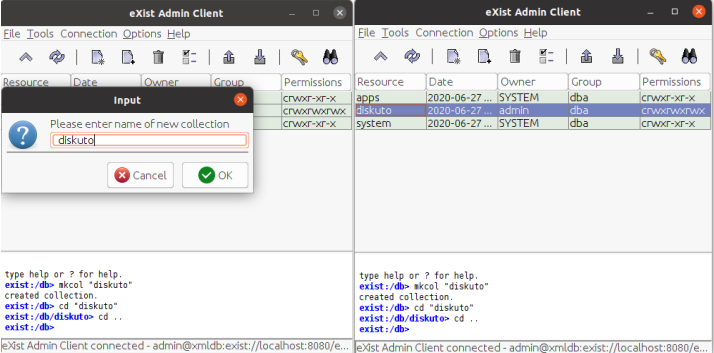
\includegraphics[width=1\textwidth]{slike/kreiranje-kolekcije.png}
    \caption{Kreiranje nove kolekcije u bazi podataka}
\end{figure}

Dvostrukim klikom na nju otvara se sadržaj odabrane kolekcije. Inicijalno nema ništa u njoj, pa je potrebno definirati XML dokumente kojima će aplikacija pristupati. U kolekciji je moguće, osim dokumenata i novih kolekcija, dodavati bilo koje druge direktorije ili datoteke različitih formata koji su pohranjeni na računalu na kojem se nalazi baza podataka. Novi direktoriji ili datoteke se dodaju odabirom u izborniku "File -> Store files/directories" ili pritiskom na "Ctrl + S". Za potrebe projektnog dijela diplomskog rada u bazu podataka će biti samo pohranjeni XML dokumenti. Novi XML dokument se može uvesti na prethodno objašnjeni način ili se izravno kreirati u Java Admin Clientu odabirom u izborniku "File -> Create blank document" ili pritiskom na "Ctrl + B". Kao novi resurs može se kreirati XML dokument ili XQuery Module. Nakon što se zada naziv dokumenta (bez ekstenzije .xml), potrebno je pritisnuti gumb "Create Resource" i dokument se sprema u bazu. Na ovaj način kreirat će se svi potrebni XML dokumenti za rad aplikacije: forums.xml, messages.xml, posts.xml i users.xml.

\begin{figure}[h!]
    \centering
    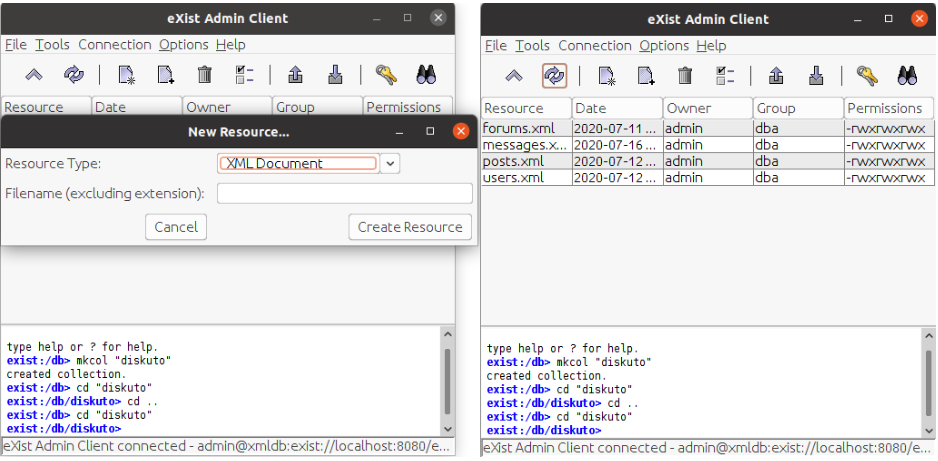
\includegraphics[width=1\textwidth]{slike/kreiranje-dokumenta.png}
    \caption{Kreiranje novog dokumenta u bazi podataka}
\end{figure}

Da bi vanjske aplikacije mogle pristupati pojedinim kolekcijama, dokumentima i drugim datotekama u bazi podataka, potrebno je postaviti dozvole za čitanje, pisanje i izvršavanje sadržaja. Promjena dozvola se vrši na način da se u alatnoj traci eXist-db odabere u glavnom izborniku "File -> Resource properties" ili pritiskom na "Ctrl + P", pri čemu se otvara prozor prikazan kao na slici \ref{properties}. Moguće je vidjeti detalje o odabranom sadržaju: naziv resursa, tip podatka, datum i vrijeme kreiranja, datum i vrijeme zadnje promjene, veličinu i sažetak sadržaja. Moguće je promijeniti vlasnika i grupu sadržaja, te mijenjati prava pristupa za vlasnika, grupu i sve druge korisnike.

\begin{figure}[h!]
    \centering
    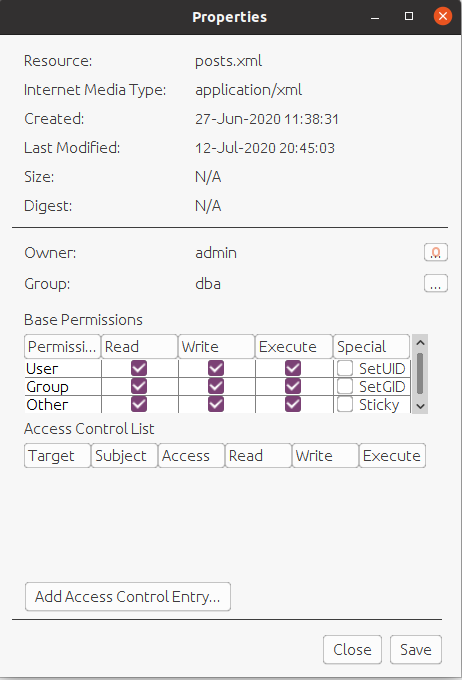
\includegraphics[width=0.5\textwidth]{slike/postavke-dokumenta.png}
    \caption{Promjena postavki XML dokumenta}
    \label{properties}
\end{figure}

Dvostrukim klikom na dokument otvara se uređivač XML dokumenta. Nad svakim dokumentom je potrebno zadati korijenski element; u dokumentu "forums.xml" će to biti "<forums/>", u "messages.xml" će to biti "<messages/>", u "posts.xml" će to biti "<posts/>" i u "users.xml" će to biti "<users/>". Od ostalih opcija koje se nalaze u Java Admin Clientu moguće je brisati dokumente ili kolekcije (preko glavnog izbornika "FIle -> Remove" ili "Ctrl + D"), kopirati dokumente ili kolekcije (preko glavnog izbornika "File -> Copy" ili "Ctrl + C"), premještati dokumente ili kolekcije na drugu lokaciju unutar baze podataka (preko glavnog izbornika "File -> Move" ili "Ctrl + M"), preimenovati dokumente ili kolekcije (preko glavnog izbornika "File -> Rename" ili "Ctrl + R"), izvesti resurs iz baze na memoriju računala (preko glavnog izbornika "File -> Export a resource to file..." ili "Ctrl + E"), dodavati okidače u bazi (preko glavnog izbornika "Tools -> Edit Triggers" ili "Ctrl + T"), uređivati popis korisnika baze podataka (preko glavnog izbornika "Tools -> Edit Users" ili "Ctrl + U"), te gasiti ili pokretati vezu prema bazi podataka (preko glavnog izbornika "Connection").  \cite{exist}

Nakon kreiranja baze podataka, potrebno je kreirati projekt kao Java web-aplikacija na kojem će se izraditi programsko rješenje koje će koristiti kreiranu bazu podataka. Potrebno je kreirati i pomoćne klase preko kojih će ostali dijelovi aplikacije pristupati bazi podataka i preko kojih će dohvaćeni podaci iz XML formata moći biti vraćeni kao čisti podaci bez XML obilježja. Kao programski isječak \ref{Database.java} prikazan je sadržaj pomoćne klase "Database.java" za rad sa bazom podataka, a kao programski isječak \ref{XmlHelper.java} prikazan je sadržaj pomoćne klase "XmlHelper.java" za rad sa podacima u XML formatu.

\begin{lstlisting}[language=Java, numbers=left, caption=Sadržaj pomoćne klase "Database.java", captionpos=b, label={Database.java}]
package org.diskuto.helpers;

import org.exist.xmldb.EXistXQueryService;
import org.xmldb.api.DatabaseManager;
import org.xmldb.api.base.Collection;
import org.xmldb.api.base.ResourceSet;
import org.xmldb.api.base.XMLDBException;

public class Database {

    private final String URI = "xmldb:exist://localhost:8080/exist/xmlrpc";
    private final String driver = "org.exist.xmldb.DatabaseImpl";
    private final String collection = "/db/diskuto";
    private final org.xmldb.api.base.Database database;
    private final Collection col;

    public Database() throws ClassNotFoundException, InstantiationException, IllegalAccessException, XMLDBException {
        Class c = Class.forName(driver);
        database = (org.xmldb.api.base.Database) c.newInstance();
        DatabaseManager.registerDatabase(database);
        col = DatabaseManager.getCollection(URI + collection, "admin", "");
    }

    public void close() throws XMLDBException {
        col.close();
        DatabaseManager.deregisterDatabase(database);
    }

    public ResourceSet xquery(String upit) throws XMLDBException {
        EXistXQueryService service = (EXistXQueryService) col.getService("XQueryService", "1.0");
        service.setProperty("indent", "yes");
        return service.query(upit);
    }

}
\end{lstlisting}

Preporučeni način za rad sa eXist-db prilikom razvijanja Java aplikacija je korištenje XML:DB API koji pruža zajedničko sučelje za rad s NXD i XED bazama podataka i podržava razvoj aplikaciju za višekratnu upotrebu. Na početku je potrebno uvesti biblioteke za rad sa bazom koje se mogu naći u direktoriju sa bibliotekama eXist-db (linije 3-7).  Klasa sadrži nekoliko finalnih varijabli koje su definirane linijama 11-15. U liniji 11 je definiran URI za pristup bazi podataka koji općenito mora biti u formatu "xmldb:exist//[HOST-ADDRESS]/db/kolekcija". Budući da više od jednog upravljačkog programa baze podataka se može registrirati u upravitelj baze podataka, potreban je dio URI-ja "xmldb:exist" da bi se utvrdilo koju klasu upravljačkih programa treba koristiti. Pod [HOST-ADDRESS] upisuje se adresa i port na kojem se nalazi baza podataka. Završni dio URI-ja definira kolekciju kojoj se pristupa. \cite{existdb-java} U liniji 12 je definiran naziv upravljača pomoću kojeg se može raditi sa bazom podataka. U liniji 13 definirana je kolekcija u kojoj se nalaze XML dokumenti sa kojima se radi u aplikaciji. Varijabla se kasnije povezuje sa URI-jem kako bi se dobila konačna putanja prema kolekciji u bazi podataka. U liniji 14 i 15 se definiraju objekti baze podataka i kolekcije.

Klasa se sastoji od konstruktora i dvije metode: "close" i "xquery". Prilikom poziva konstruktora kada se inicijalizira novi objekt klase "Database", registrira se nova instanca klase upravljača (linije 18-20) i od upravitelja baze podataka se dohvaća kolekcija pozivanjem statičke metode "DatabaseManager.getCollection" (linija 21). Metoda kao argument prima URI do kolekcije, te korisničko ime i lozinku za prijavu u bazu podataka. Nakon uspješne inicijalizacije nad bazom podataka se mogu vršiti upiti pomoću metode "xquery" koja kao argument prima XQuery upit.  Za rad sa upitima koristi se XQueryService klasa eXista (linija 30) koja se može pozvati preko metode "getService" klase Collection. Metoda prima naziv usluge kao prvi argument i njegovu verziju kao drugi argument.  Za izvršenje upita poziva se metoda "query" nad inicijaliziranim servisom (linija 32). Metoda prima upit u formatu stringa, a vraća objekt ResourceSet. Nakon što se završi sa radom, poželjno je osloboditi zauzete resurse pozivom metode "close" koja zatvara kolekciju (linija 25) i deregistrira bazu podataka sa upravitelja baze podataka (linija 26).

Nakon dohvaćanja XML-a preko upita iz klase "Database", potrebno je izvući dobivene podatke iz XML elemenata što se može učiniti pomoću metoda iz klase "XmlHelper". Klasa sadrži četiri metode za dohvaćanje podataka iz XML resursa koji se pri instanciranju klase proslijeđuje u konstruktor. U klasi se nalaze dvije varijable: "xml" u kojoj se pohranjuje XML zapis dobivenog resursa i "xp" pomoću kojeg se prolazi i dohvaćaju čvorovi XML resursa. U nastavku slijedi prikaz i pojašnjenje klase.

\begin{lstlisting}[language=Java, numbers=left, caption=Sadržaj pomoćne klase "XmlHelper.java", captionpos=b, label={XmlHelper.java}]
package org.diskuto.helpers;

import java.io.StringReader;
import java.util.ArrayList;
import java.util.List;
import javax.xml.xpath.XPath;
import javax.xml.xpath.XPathConstants;
import javax.xml.xpath.XPathExpressionException;
import javax.xml.xpath.XPathFactory;
import org.w3c.dom.NodeList;
import org.xml.sax.InputSource;
import org.xmldb.api.base.Resource;

public class XmlHelper {

    XPath xp;
    String xml;

    public XmlHelper(Resource resource) throws Exception {
        this.xml = (String) resource.getContent();
        this.xp = XPathFactory.newInstance().newXPath();
    }

    public Object makeObject(String object) throws XPathExpressionException {
        return xp.evaluate("/" + object, new InputSource(new StringReader(xml)), XPathConstants.NODE);
    }

    public String makeValue(String attribute, Object object) throws XPathExpressionException {
        return xp.evaluate(attribute, object);
    }

    public List<String> makeListValue(String expression) throws XPathExpressionException {
        List<String> list = new ArrayList();
        NodeList nodes = (NodeList) xp.evaluate(expression, new InputSource(new StringReader(xml)), XPathConstants.NODESET);

        for (int i = 0; i < nodes.getLength(); i++) {
            list.add(nodes.item(i).getTextContent());
        }

        return list;
    }

    public String rawValue() {
        return xml;
    }
}
\end{lstlisting}

Na početku je potrebno uvesti nekoliko biblioteka koje su potrebne za pravilan rad klase (linije 3-12). Klasa StringReader (linija 3) sadrži metode i varijable za čitanje tekstualnog niza sinkrono ili asinkrono. Klase ArrayList (linija 4) i List (linija 5)  sadrže metode i varijable za pohranu podataka u listu. Klase iz paketa "javax.xml.xpath.*" (linije 6-9) sadrže metode i varijable za čitanje i navigaciju prema dijelovima XML dokumenta. Sučelje NodeList (linija 10) pruža apstrakciju kolekcije čvorova bez definiranja ili ograničavanja načina na koji se ova zbirka provodi. Klasa InputSource (linija 11) omogućuje aplikaciji da kapsulira informacije o ulaznom izvoru objekta, što može sadržavati razne identifikatore i znakovne tokove. Klasa Resource (linija 12) omogućuje pohranjivanje jednog resursa iz ResourceSet skupa resursa. 

Klasa XmlHelper ima konstruktor koji prima objekt tipa Resource iz kojeg se dohvaća sadržaj i sprema u varijablu "xml" (linija 20). Nakon toga se u konstruktoru vrši stvaranje nove instance objekta XPath (linija 21). Metoda "makeObject" prima naziv elementa ili putanju prema elementu kojeg se želi dohvatiti, te vraća taj element kao objekt (linija 25). Pomoću metode "makeValue" se iz objekta dobivenog preko prošle metode mogu dohvatiti vrijednost elementa kojeg taj objekt sadrži (linija 29). Metodi se kao argument proslijeđuje naziv elementa i objekt. Metodom "makeListValue", prema putanji elementa zadanom kao argument, se u listu spremaju sve vrijednosti tog elementa (linije 32-41). Posljednja metoda je "rawValue" koja vraća u tekstualnom formatu zapis XML resursa proslijeđenom konstruktoru u istom obliku kojem postoji u bazi podataka (linija 44).

\section{Java web-aplikacija}

Web aplikacija je implementirana u programskom jeziku Java, verzije Java EE 8 Web i izvršava se na poslužitelju GlassFish 5.1., a razvojni okvir u kojem se radi aplikacija je JSF 2.3. Razvojno okruženje u kojem je aplikacija razvijana je Apache NetBeans 12.0. Projekt je podijeljen u pet izvornih paketa u kojima se nalaze klase koje služe kao poslovna logika aplikacije:

\begin{itemize}
\item \textbf{org.diskuto.beans} - sadrži komponente na strani poslužitelja zadužene za učahurenje dijela poslovne logike aplikacije.
\begin{itemize}
        \item BeanHelper - pomoćno zrno čije metode Facelets mogu koristiti. Metode koje sadrži zrno su: "getActiveUser" (dohvaća objekt trenutno prijavljenog korisnika u aplikaciji), "date" (pretvara UNIX vrijeme u format datuma), "fullDate" (pretvara UNIX vrijeme u format datum i vrijeme), "retrieveDiskuto" (vraća objekt foruma sa zadanim nazivom u argumentu), "subscribe" (pretplaćuje se ili ukida pretplatu na forum zadan kao argument).
	\item ConfirmRegistration - zrno koje se koristi prilikom potvrde registracije. Sadrži varijable "insertedCode" u kojem se zapisuje kod za potvrdu registracije kojeg korisnik unese i "errorText" u kojem se zapisuje tekst pogreške koji se korisniku prikazuje. Metode koje sadrži zrno su: "validate" (provjerava ispravnost unesenog koda i potvrđuje registraciju ili ispisuje grešku u slučaju pogreške) i  "sendNewMail" (šalje elektroničku poštu sa kodom za potvrdu registracije).
	\item Discover - zrno koje se koristi prilikom pretraživanja foruma u aplikaciji. Sadrži varijablu "diskutos" u kojoj u konstruktoru pohranjuje popis foruma iz baze podataka.
	\item EditDiskuto - zrno za kreiranje i uređivanje foruma. Postoje varijable koje sadrže sve elemente iz XML Scheme za dokument "forums.xml". U konstruktoru se provjerava je li forum zadan kao parametar postoji već u bazi podataka, te ako postoji tada će varijablama pridružiti odgovarajuće vrijednosti iz baze podataka. Zrno sadrži metode "addCategory" koji dodaje kategoriju u listu, "dropCategory" koji briše kategoriju iz liste, "addModerator" koji dodaje moderatora u listu, "dropModerator" koji briše moderatora iz liste, "check" koji provjerava ispravnost unesenih podataka i "save" koji sprema podatke u bazu podataka.
	\item Forum - zrno koje se koristi za ispis stranice foruma. Sadrži varijable "diskuto" i "category" koje u konstruktoru se provjeravaju postoje li kao parametri, te se dohvaćaju. Na kraju se provjerava ukupan broj objava u forumu i poziva metoda "loadItems" koja učitava objave. U zrnu još postoji metoda "freshPost" koja u argumentu proslijeđenu kategoriju vraća najnoviju objavu.
	\item Home - zrno koje se koristi pri ispisu početne stranice aplikacije. Sadrži varijablu "messageUsers" koja ispisuje listu korisnika sa kojim korisnik ima nepročitane poruke, "unread" koja ispisuje broj nepročitanih poruka, te ostale varijable koje se koriste pri učitavanju objava pozivom metode "loadItems".
	\item Language - pomoćno zrno koje se koristi pri dohvaćanju i promjeni jezika aplikacije.
	\item Login - zrno koje se koristi prilikom korištenja stranice za prijavu korisnika u aplikaciju. Sadrži varijable "username" i "password" u koje se pohranjuju unešeni korisnički podaci prilikom prijave. U metodi "doLogin" provodi se provjera ispravnosti prijave i eventualno se ispisuju greške kroz varijablu "errorText". Metodom "logout" odjavljuje se trenutno prijavljeni korisnik.
	\item Message - zrno koje se koristi prilikom korištenja stranice za slanje i primanje privatnih poruka od drugih korisnika. Sadrži atribute "me" koji poprima istinitu vrijednost ako je prijavljeni korisnik odabrani korisnik, "ignored" koji poprima istinitu vrijednost ako je odabrani korisnik na listi blokiranih korisnika, "messages" u kojoj se nalazi popis svih poruka sa odabranim korisnikom dohvaćenih u konstruktoru zrna, "chatting" u kojoj se nalazi popis svih korisnika sa kojima je prijavljeni korisnik u prošlosti komunicirao (puni se preko metode "fillIn"), "reply" u koji se pohranjuje poruka koja se šalje metodom "send".
	\item MyDiskuto - zrno koje se koristi pri ispisu popisa vlastitih foruma. Sadrži varijable "owner" u kojoj se nalazi popis foruma kojih je korisnik vlasnik, te "moderator"u kojem se nalazi popis foruma kojih je korisnik moderator. Navedene varijable se pune pozivom u konstruktoru metode "fillIn".
	\item NewPassword - zrno koje se koristi prilikom poništavanja korisničke lozinke. Sadrži varijable "state" koja definira u kojoj fazi se nalazi korisnik u poništavanju lozinke, "email" u kojoj se definira elektronička pošta korisnika kojeg se metodom "abolishPassword" poništava lozinka, "code" koji služi za autentikaciju korisnika, "password" i "rpassword" u kojima se pohranjuje nova lozinka korisnika metodom "addNewPassword" i "errorText" koji služi za ispis eventualnih grešaka. U zrnu se nalazi još metoda "check" koja provjerava ispravnost unesene nove lozinke.
	\item NewPost - zrno koje se koristi kod kreiranja nove objave na određenom forumu. Postoje varijable koje sadrže sve elemente iz XML Scheme za dokument "posts.xml". U konstruktoru se dohvaća forum proslijeđen kao parametar, te ako on ne postoji korisnika se preusmjerava na stranicu koja obavještava o pogreški. Metodom "save" se provjerava ispravnost unešenih podataka, te ako je sve u redu objava se sprema u bazu podataka.
	\item Post - zrno koje prikazuje objavu i komentare objave. Sadrži varijable "main" koja u konstruktoru dohvaća forum na kojem je objava objavljena, "thing" koja u konstruktoru dohvaća objavu prema zadanom parametru, "comments" u kojem se spremaju komentari objave i "myComment" u kojem se pohranjuje komentar korisnika koji se šalje metodom "sendComment". U zrnu postoje još metode "reportPost" pomoću koje se može prijaviti objava, "reportComment" pomoću koje se može prijaviti komentar, "deletePost" pomoću koje se može obrisati objava, "deleteComment" pomoću koje se može obrisati komentar, "lock" pomoću koje se može zaključati objava, "unlock" pomoću koje se može otključati objava, "upvotePost" pomoću koje se može objava označiti sa +, "downvotePost" pomoću koje se objava može označiti sa -, "upvoteComment" pomoću koje se komentar može označiti sa + i "downvoteComment" pomoću koje se komentar može označiti sa -.
	\item Profile - zrno koje se koristi za ispis profila određenog korisnika. Sadrži varijable "user" u kojoj su zapisani svi podaci korisnika koji se dohvaćaju u konstruktoru, "me" koji poprima istinitu vrijednost ako je prijavljeni korisnik odabrani korisnik, "upvotes" broj + oznaka korisnika, "downvotes" broj - oznaka korisnika, "totalPosts" ukupan broj objava, "totalComments" ukupan broj komentara, "post" u kojem se spremaju objave, "comments" u kojem se spremaju komentari, "postsIteratorId" i "commentsIteratorId" koje služe za pomoć pri učitavanju objava i komentara preko metoda "loadPosts" i "loadComments". U zrnu postoji metoda "ignore" koja stavlja odabranog korisnika na listu za ignoriranje.
	\item Registration - zrno koje se koristi prilikom registracije novog korisnika. Sadrži varijable "email", "username", "password" i "rpassword" koje korisnik unosi prilikom registracije. Varijablom "errorText" se ispisuje eventualna pogreška nastala provjerom unosa preko metode "check". Metodom "doRegistration" vrši se registracija i sprema se novi korisnik u bazu.
	\item Reports - zrno koje se prikazuje prijavljene objave i komentare na određenom forumu. Sadrži varijable "diskuto" u kojem se pohranjuju podaci o odabranom forumu, "items" koja sadrži popis prijavljenih objava i "comments" koja sadrži popis prijavljenih komentara. Metodom "deletePost" se briše odabrana objava, "deleteComment" se briše odabrani komentar, "okPost" se označava da je objava primjerena i briše se sa popisa prijavljenih objava i metodom "okComment" se označava da je komentar primjeren i briše se sa popisa prijavljenih komentara.
	\item Search - zrno koje se koristi prilikom pretrage. Sadrži varijable "term" u kojoj se zapisuje ključna riječ za pretragu, "userResults" u kojoj se zapisuju korisnici čije korisničko ime ima u sebi ključnu riječ, "diskutoResults" u kojoj se zapisuju forumi čiji nazivi imaju u sebi ključnu riječ, "postResults" u kojoj se zapisuju objave čiji nazivi imaju u sebi ključnu riječ. Metodom "showResults" se prikazuje pretraga po ključnoj riječi.
	\item Settings - zrno koje se koristi kod promjene postavki korisnika. Sadrži varijable "username" u kojoj se pohranjuje korisničko ime prijavljenog korisnika, "email" u kojem se pohranjuje elektronička pošta korisnika, "wantEmail" koji se postavlja na istinitu vrijednost kada korisnik metodom "changeEmail" želi promijeniti svoj e-mail, "wantPassword" koji se postavlja na istinitu vrijednost kada korisnik metodom "changePassword" želi promijeniti svoju lozinku, "wantDisable" koji se postavlja na istinitu vrijednost kada korisnik metodom "disableAccount" želi obrisati svoj korisnički račun.
\end{itemize}
\item \textbf{org.diskuto.helpers} - sadrži pomoćne klase za rad koje koriste zrna i ostali dijelovi aplikacije. Osim već objašnjenih klasa "Database" i "XmlHelper", u paketu se nalaze sljedeće klase:
\begin{itemize}
	\item AppHelper - sadrži metode "getActiveUser" koja vraća trenutno prijavljenog korisnika u aplikaciji, "param" koja vraća vrijednost parametra iz Faces konteksta prema zadanom ključu, "getOutput" koja za zadani ključ vraća pripadajući tekstualni niz kod datoteka internacionalizacije, "checkLogged" koja provjerava postoji li prijavljeni korisnik u aplikaciji, "getAttachmentsPath" koja vraća putanju prema direktoriju "attachments" u aplikaciji, "generateId" koja generira jedinstveni identifikator u bilo kojem XML dokumentu, "date" koja pretvara UNIX vrijeme u format običnog datuma, "fullDate" koja pretvara UNIX vrijeme u format datum i vrijeme, "getResourceSet" koja poziva bazu podataka i vraća skup resursa za definirani upit, "getResource" koja poziva bazu podataka i vraća prvi resurs za definirani upit, "login" koja poziva bazu podataka i provjerava jesu li proslijeđeni podaci za prijavu ispravni, "usernameExist" koja poziva bazu podataka i provjerava postoji li korisnik sa proslijeđenim korisničkim imenom u bazi, "forumExist" koja poziva bazu podataka i provjerava postoji li forum sa zadanim nazivom u bazi, "regex" koji vrši provjeru regularnim izrazom.
	\item MailHelper - pomoćna klasa za slanje e-mail poruka. Sadrži varijable "to" koja označava e-mail korisnika kojem se šalje mail, "subject" koja označava predmet i "text" koja označava sadržaj elektroničke pošte. Vrijednosti varijabli se postavljaju pri instanciranju novog objekta klase. Klasa sadrži metodu "sendMail" koja na navedeni mail šalje poruku sa definiranim predmetom i tijelom poruke.
	\item Retriever - pomoćna klasa koja služi za dohvaćanje objekata iz baze podataka. Sadrži varijablu "key" koja predstavlja ključ za dohvaćanje pojedinog podatka, a vrijednost varijable se postavlja pri instanciranju novog objekta klase. U klasi se nalaze metode: "user" koja dohvaća korisnika iz baze podataka sa određenim korisničkim imenom, "forum" koja dohvaća forum iz baze podataka sa određenim nazivom foruma, "post" koja dohvaća objavu iz baze podataka sa određenim nazivom objave, "messages" koja dohvaća listu poruka koje trenutno prijavljeni korisnik ima sa određenim korisnikom, "searchUsers" koja dohvaća sve korisnike koji u svom korisničkom imenu sadrže određenu ključnu riječ, "searchForum" koja dohvaća sve forume koji u svom nazivu sadrže određenu ključnu riječ, "searchPosts" koja dohvaća sve objave koje u svom nazivu sadrže određenu ključnu riječ.
\end{itemize}
\item \textbf{org.diskuto.listeners} - paket koji sadrži klasu "Listener" u kojoj se sluša životni ciklus web aplikacije. Sadrži jednu javnu statičku varijablu "sc" u kojoj se prilikom inicijalizacije sprema kontekst servleta. Pomoću konteksta se može komunicirati sa servlet containerom. Klasa sadrži metode za zapisivanje, brisanje i dohvaćanje varijabli iz sesije: "addToSession" upisuje u sesiju objekt pod zadanim atributom, "deleteFromSession" briše iz sesije objekt pod zadanim atributom, "getFromSession" dohvaća objekt iz sesije pod zadanim atributom.
\item \textbf{org.diskuto.models} - paket koji preslikava modele dokumenata iz baze podataka. Svaka klasa sadrži atribute definirane u XML Schemi kojima se dodijeljuju vrijednosti pozivom metode "retrieve" proslijeđivanjem objekta klase XmlHelper u kojem se nalazi XML zapis dohvaćen iz baze podataka. Svaka klasa ima metode za pridruživanje i postavljanje vrijednosti varijablama klase. Od ostalih metoda, klasa Comment sadrži: "save" pomoću kojeg se sprema komentar u bazu podataka, "addVote" pomoću kojeg se postavlja + ili - za komentar, "dropVote" pomoću kojeg se briše + ili - sa komentara, "post" pomoću kojeg se dohvaća objekt Post za komentar, "report" pomoću kojeg se prijavljuje komentar, "itsOk" pomoću kojeg se briše komentar sa liste prijava, "delete" pomoću kojeg se briše komentar. Klasa Forum još sadrži metode "save" kojom se sprema novi forum u bazu podataka i "update" kojom se ažurira forum u bazi podataka. Klasa Message sadrži metodu "send" pomoću koje se šalje privatna poruka od određenog pošiljatelja prema određenom primatelju uz određeni tekst poruke. Klasa Post sadrži metode "save" kojom se objava sprema u bazu podataka, "addVote" pomoću kojeg se postavlja + ili - za objavu, "dropVote" pomoću kojeg se briše + ili - sa objave, "report" pomoću kojeg se prijavljuje objava, "itsOk" pomoću kojeg se briše objava sa liste prijava, "delete" pomoću kojeg se briše objava, "lock" kojom se zaključava objava i "unlock" kojom se otključava objava. Klasa User još sadrži metode "register" kojom se sprema novi korisnik u bazu podataka, "login" kojom se prijavljuje korisnik u aplikaciju, "logout" kojom se odjavljuje korisnik iz aplikacije, "disable" kojom se briše korisnički račun, "sendConfirmMail" kojom se šalje e-mail za potvrdu korisničkom računa, "confirmUser" kojom se potvrđuje korisnički račun, "changeLanguage" kojom se zapisuje promjena jezika u bazi podataka, "subscribe" kojom se korisnik pretplaćuje na određeni forum, "unsubscribe" kojom korisnik ukida pretplatu sa određenog foruma, "ignore" kojom se stavlja određeni korisnik na listu za ignoriranje i "unignore" kojom se briše korisnik sa liste za ignoriranje.
\item \textbf{org.diskuto.translations} - u paketu se nalaze datoteke tipa Properties u kojima se za svaki jezik koji podržava aplikacija (engleski kao zadani i hrvatski) nalaze atributi kojima se pridružuju sadržaji za ispis na pojedinim web stranicama. Datoteke koje se nalaze u paketu su: "language.properties" (za zadani jezik), "language\_en.properties" (za engleski jezik) i "language\_hr.properties" (za hrvatski jezik).
\end{itemize}

Od ostalih datoteka u Java web-aplikaciji nalaze se .xhtml dokumenti koji su detaljnije objašnjeni u poglavlju 8 uz prikaz snimke zaslona i detaljan opis funkcionalnosti. U aplikaciji postoje sljedeće konfiguracijske datoteke: "web.xml" (definira slušače, Faces Servlet, trajanje sesije, početnu stranicu, stranicu koja se prikazuje prilikom pogrešaka i sl.), "glassfish-web.xml" (konfiguracijska datoteka na razini poslužitelja koji izvršava aplikaciju), "faces-config.xml" (konfiguracijska datoteka na razini JSF razvojnog okvira u kojoj se deklariraju jezici i paketi za lokalizaciju). U aplikaciji postoji direktorij "resources" koji je podijeljen na nekoliko sljedećih poddirektorija:
\begin{itemize}
\item \textbf{attachments} - u direktoriju se pohranjuju slike koje se mogu učitati kao prilog prilikom kreiranja nove objave. Svaka slika ima naziv u obliku "res-<id objave>".
\item \textbf{css} - u direktoriju se nalaze .css datoteke kojim se uređuje izgled i raspored stranice.
\item \textbf{js} - u direktoriju se nalaze .js datoteke koje se izvršavaju kada aplikacija pozove Ajax zahtjev. Pomoću njih se definira pokretanje animacije na određenim mjestima prilikom čekanja na dovršavanje zadatka kojeg aplikacija izvršava.
\item \textbf{pages} - u direktoriju se nalaze razne dodatne vanjske datoteke i slike poput ikone aplikacije, animacije koja se pokreće prilikom čekanja na dovršavanje zadatka kojeg aplikacija izvršava, te razne druge ikone i logotipi.
\end{itemize}

\chapter{Primjeri korištenja}

U ovom poglavlju će biti opisani primjeri korištenja izrađene web aplikacije. Svaka izrađena funkcionalnost će biti prikazana uz odgovarajuće slike zaslona i njihov opis.

\section{Početna stranica}

\begin{figure}[h!]
    \centering
    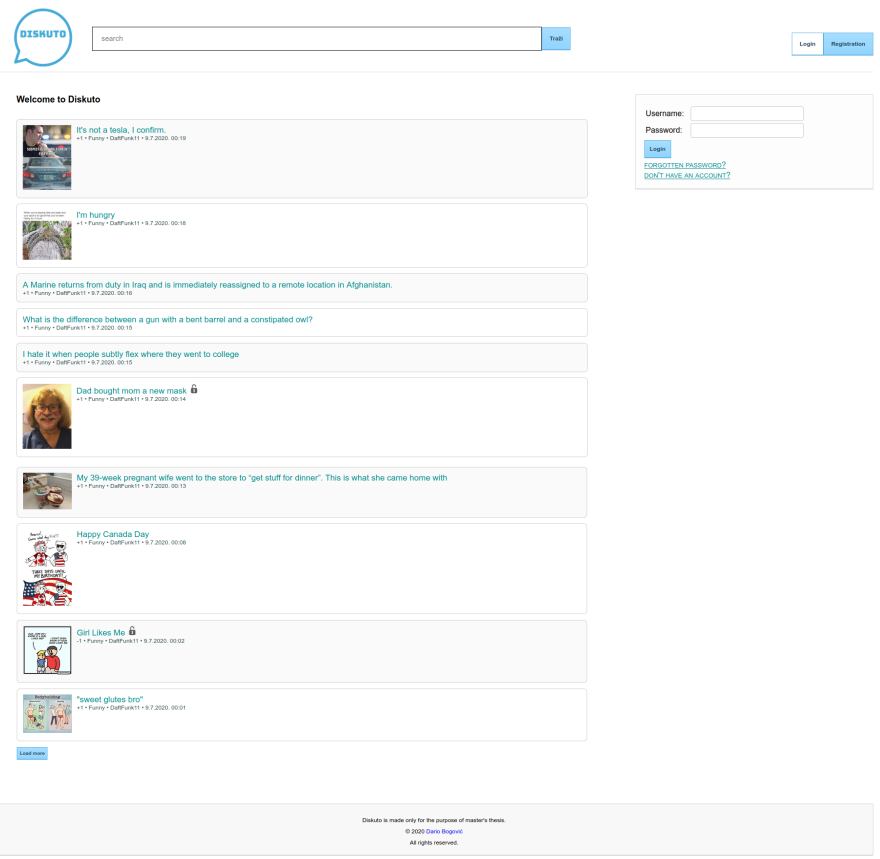
\includegraphics[width=1\textwidth]{slike/pocetna.png}
    \caption{Prikaz početne stranice (neprijavljen korisnik)}
    \label{pocetna}
\end{figure}

Na slici \ref{pocetna} je prikazana početna stranica web aplikacije. Sastoji se od tri dijela: zaglavlja stranice, podnožja stranice i glavnog dijela stranice. Zaglavlje stranice sadrži s lijeva na desno: logo, pretraživač web aplikacije i dvije poveznice koje vode na prijavu korisnika u aplikaciju ili na registraciju korisnika. Glavni dio početne stranice je prikazan u sredini i sadrži s desne strane blok element za brzu prijavu korisnika s poveznicama koje vode do forme za obnavljanje zaboravljene lozinke ili za registraciju novog korisnika. S lijeve strane glavnog dijela web aplikacije nalazi se poruka dobrodošlice i ispod koje poveznice na 10 najnovijih objava u aplikaciji. Na kraju se nalazi gumb za učitavanje dodatnih 10 objava. Podnožje stranice sadrži detalje o web aplikaciji i poveznicu na e-mail adresu autora.

\subsection{Početna stranica prijavljenog korisnika}

\begin{figure}[h!]
    \centering
    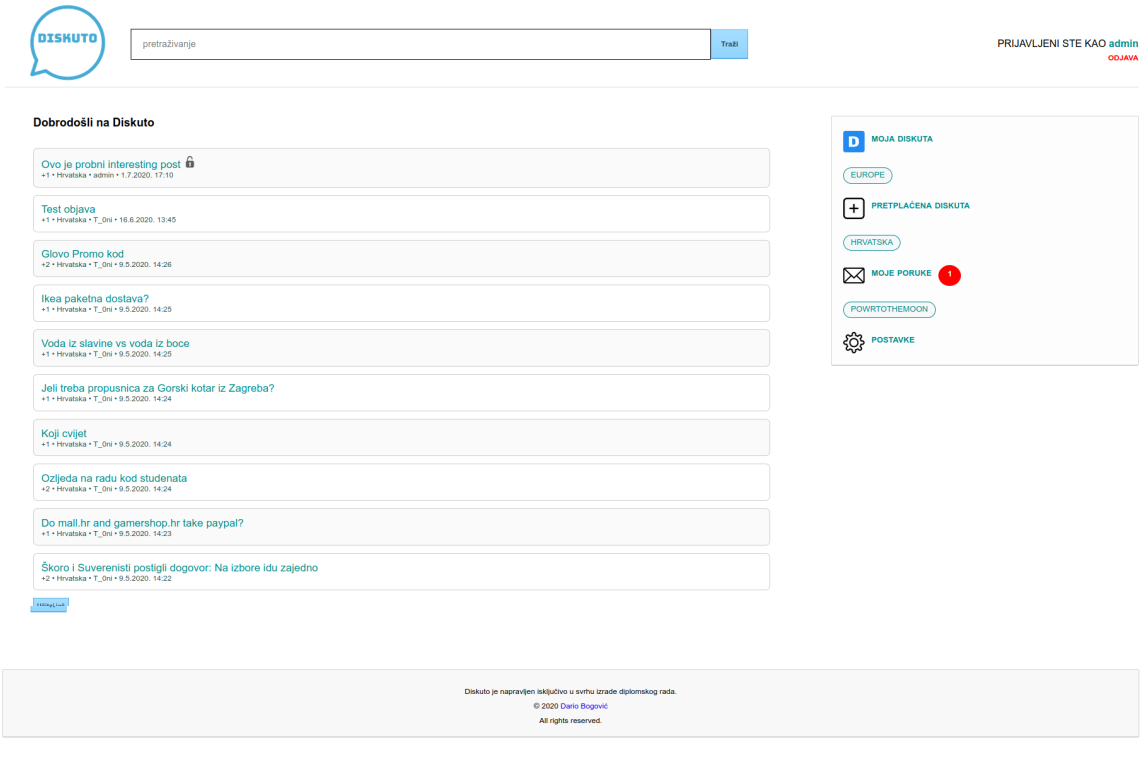
\includegraphics[width=1\textwidth]{slike/pocetna-prijavljen.png}
    \caption{Prikaz početne stranice (prijavljen korisnik)}
\end{figure}

Prijavom korisnika, bilo preko stranice namijenjene prijavi ili preko brze prijave, korisnika se preusmjerava na njegovu početnu stranicu. Za razliku od početne stranice neprijavljenog korisnika, kod prijavljenog korisnika ona sadrži u glavnom dijelu s lijeve strane popis najnovijih objava sa foruma na koje se korisnik pretplatio (za razliku od popisa najnovijih objava sa svih foruma koji se prikazuje neprijavljenom korisniku), a sa desne strane glavni izbornik sa mogućnostima. U glavnom izborniku može se odabrati opcija "Moja Diskuta" koja korisnika vodi na stranicu sa svojim kreiranim forumima na kojem može kreirati forume ili im mijenjati postavke. Ispod poveznice na opciju se nalazi popis svih vlasititih foruma, te se klikom na njih može brzo pristupiti. Sljedeća mogućnost je "Pretplaćena Diskuta" koja korisnika vodi na stranicu za otkrivanje novih foruma na koje bi se korisnik mogao pretplatiti. Ispod poveznice se nalazi popis svih foruma na koje se korisnik pretplatio, te se njima može brzo pristupiti. Mogućnost "Moje poruke" korisnika vodi do stranice sa privatnim porukama. S desne strane se može vidjeti broj nepročitanih poruka koje korisnik ima, a ispod poveznice se može brzo pristupiti razgovoru s korisnicima s kojima ima nepročitanih poruka. Zadnja opcija u glavnom izborniku su "Postavke" koje korisnika vode do stranice sa postavkama korisničkog računa. U zaglavlju stranice, s desne strane, je prikazan naziv trenutačno prijavljenog korisnika. Pritiskom na naziv otvara se javni profil korisnika. Ispod naziva, nalazi se poveznica "Odjava" koja korisnika odjavljuje iz aplikacije.

\section{Registracija}

Na početnoj stranici kod neprijavljenog korisnika, klikom na poveznicu "Registration" u zaglavlju stranice ili "Don't have an account?" u glavnom dijelu stranice, otvara se web stranica sa formom za registraciju korisnika u aplikaciji prikazana na slici \ref{registracija}.

\begin{figure}[h!]
    \centering
    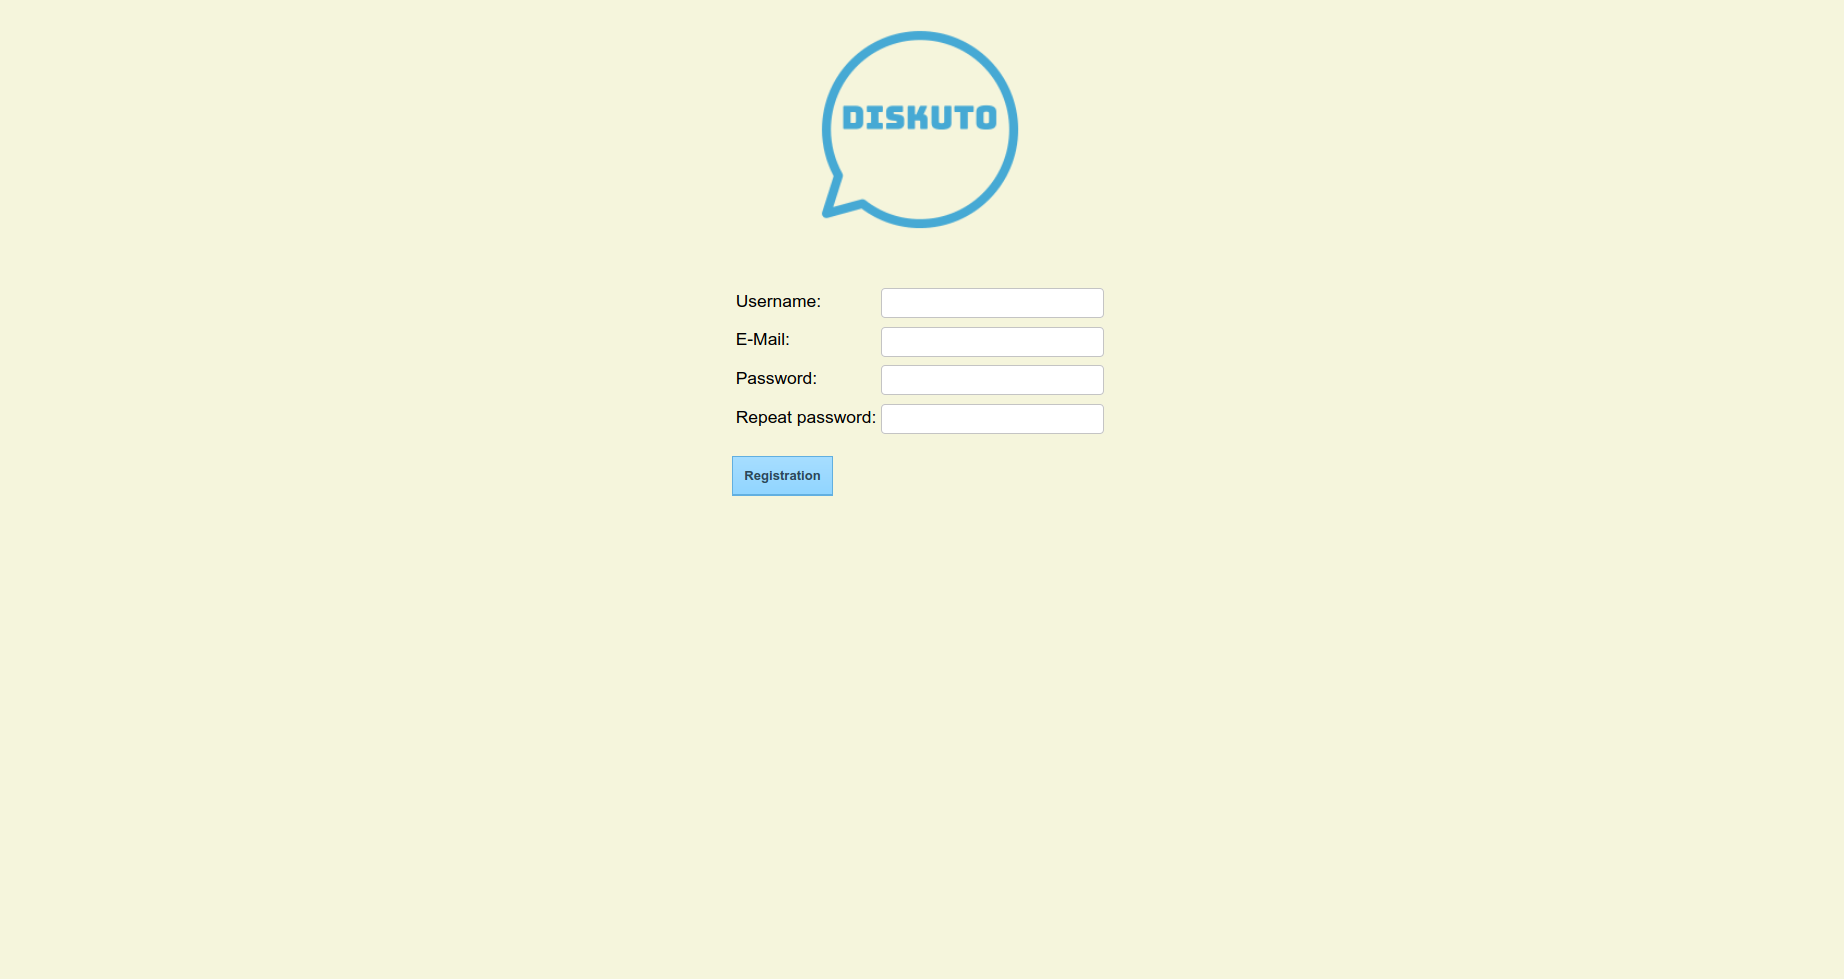
\includegraphics[width=1\textwidth]{slike/registracija.png}
    \caption{Forma za registraciju novog korisnika}
    \label{registracija}
\end{figure}

Prilikom registracije, korisnik mora unijeti željeno korisničko ime, e-mail, lozinku i ponoviti lozinku. Postoje nekoliko ograničenja prilikom registracije koja se moraju poštovati:

\begin{itemize}
\item Svi podaci moraju biti obavezno uneseni
\item Korisničko ime i e-mail ne smiju postojati u bazi; svako korisničko ime se veže za isključivo jednog korisnika, te svaki e-mail se veže isljučivo za jednog korisnika
\item Korisničko ime ne smije biti kraće od 3 znaka, lozinka ne smije biti kraća od 8 znakova, a e-mail mora biti pravilnog formata
\item Unesena lozinka i ponovljena lozinka moraju biti jednake
\end{itemize}

Ukoliko neko ograničenje nije zadovoljeno, korisniku će se na zaslon ispisati poruka sa greškom. Tek kada je sve u redu sa unešenim podacima, u bazu se spremaju podaci i korisnika se preusmjerava na formu za potvrdu registracije. U međuvremenu, korisniku se dodijeljuju još neki meta-podaci: generira se kod za potvrdu koji će korisniku biti poslan na njegov e-mail, dodijeljuje mu se datum i vrijeme kada mu je kreiran račun, te se kao jezik aplikacije postavlja se engleski. Na kraju se šalje e-mail za potvrdu registracije.

\subsection{Potvrda registracije}

\begin{figure}[h!]
    \centering
    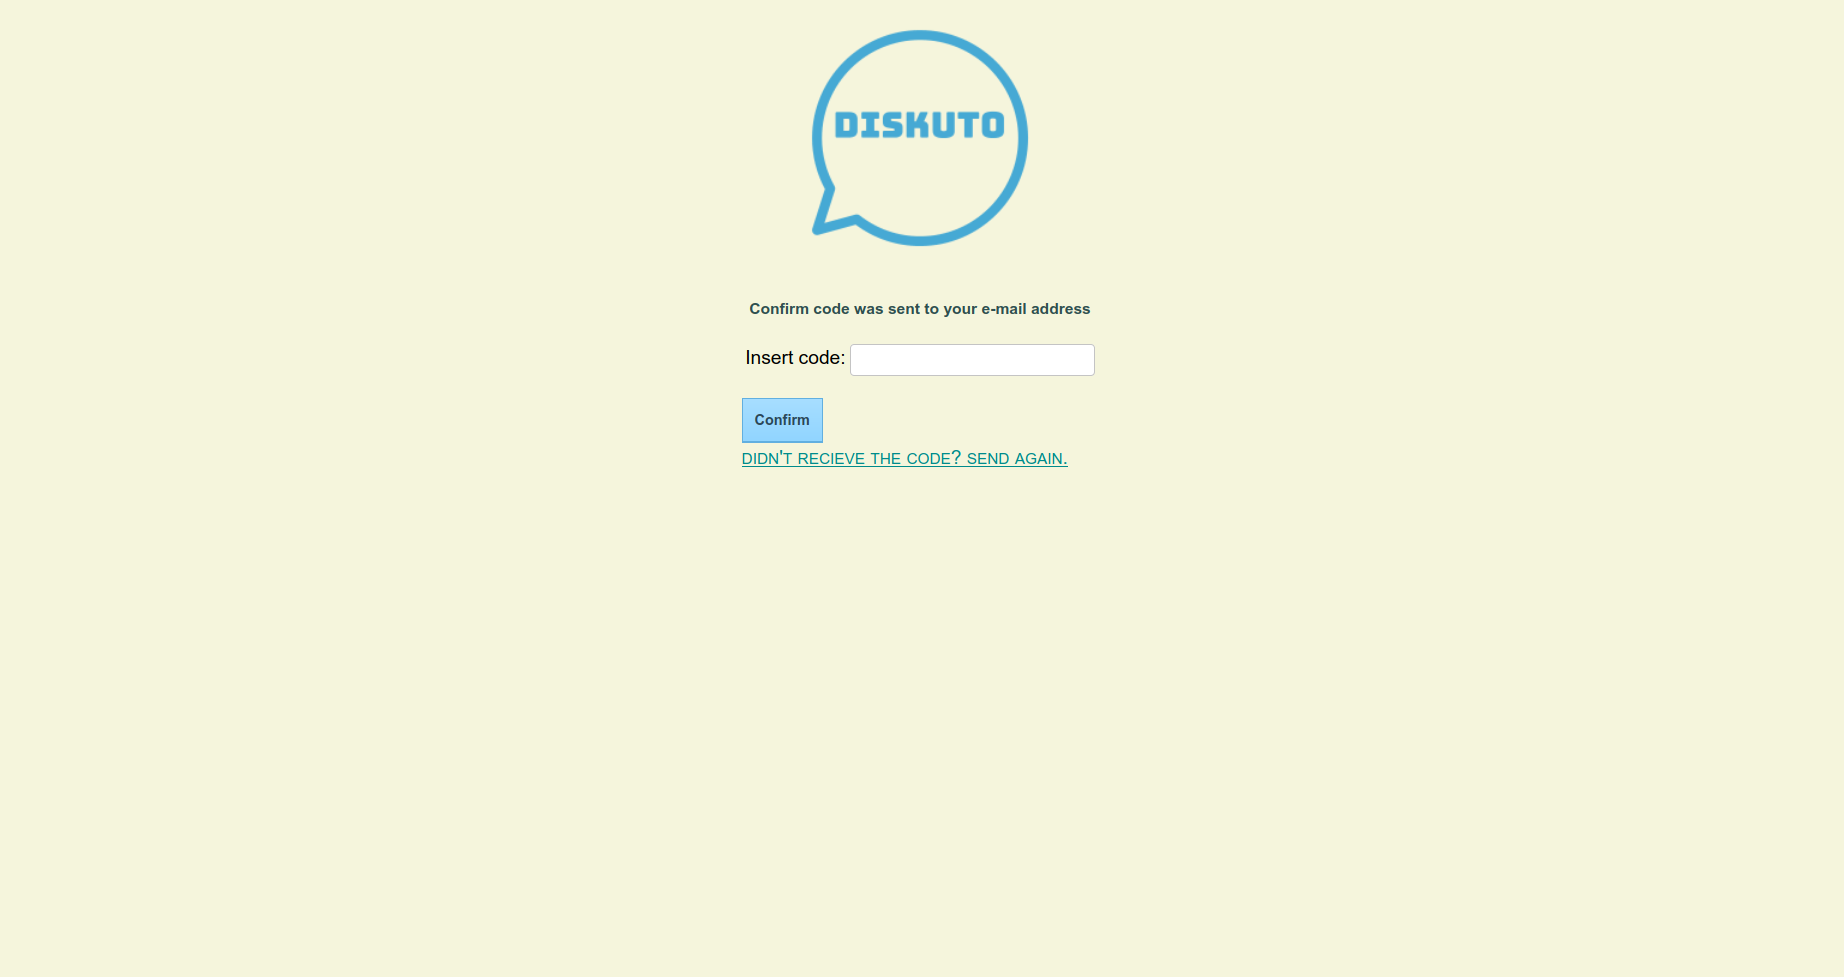
\includegraphics[width=1\textwidth]{slike/potvrda-registracije.png}
    \caption{Forma za potvrdu registracije novog korisnika}
    \label{potvrda-registracije}
\end{figure}

Na slici \ref{potvrda-registracije} je prikazana forma za potvrdu registracije novog korisnika. Kako bi potvrdio registraciju, korisnik mora unijeti šesteroznamenkasti kod kojeg je primio na mail. Ukoliko krivo unese kod, prikazuje mu se poruka greške. Ako je bilo problema oko primanja koda, korisnik može zatražiti ponovno slanje na njegov e-mail klikom na poveznicu "Send again". Tek kada unese ispravan kod, korisniku se potvrđuje registracija i postaje član Diskuta. Nepotvrđeni korisnici ne mogu se služiti aplikacijom, odnosno imaju iste ovlasti kao i drugi neregistrirani korisnici.

\begin{figure}[h!]
    \centering
    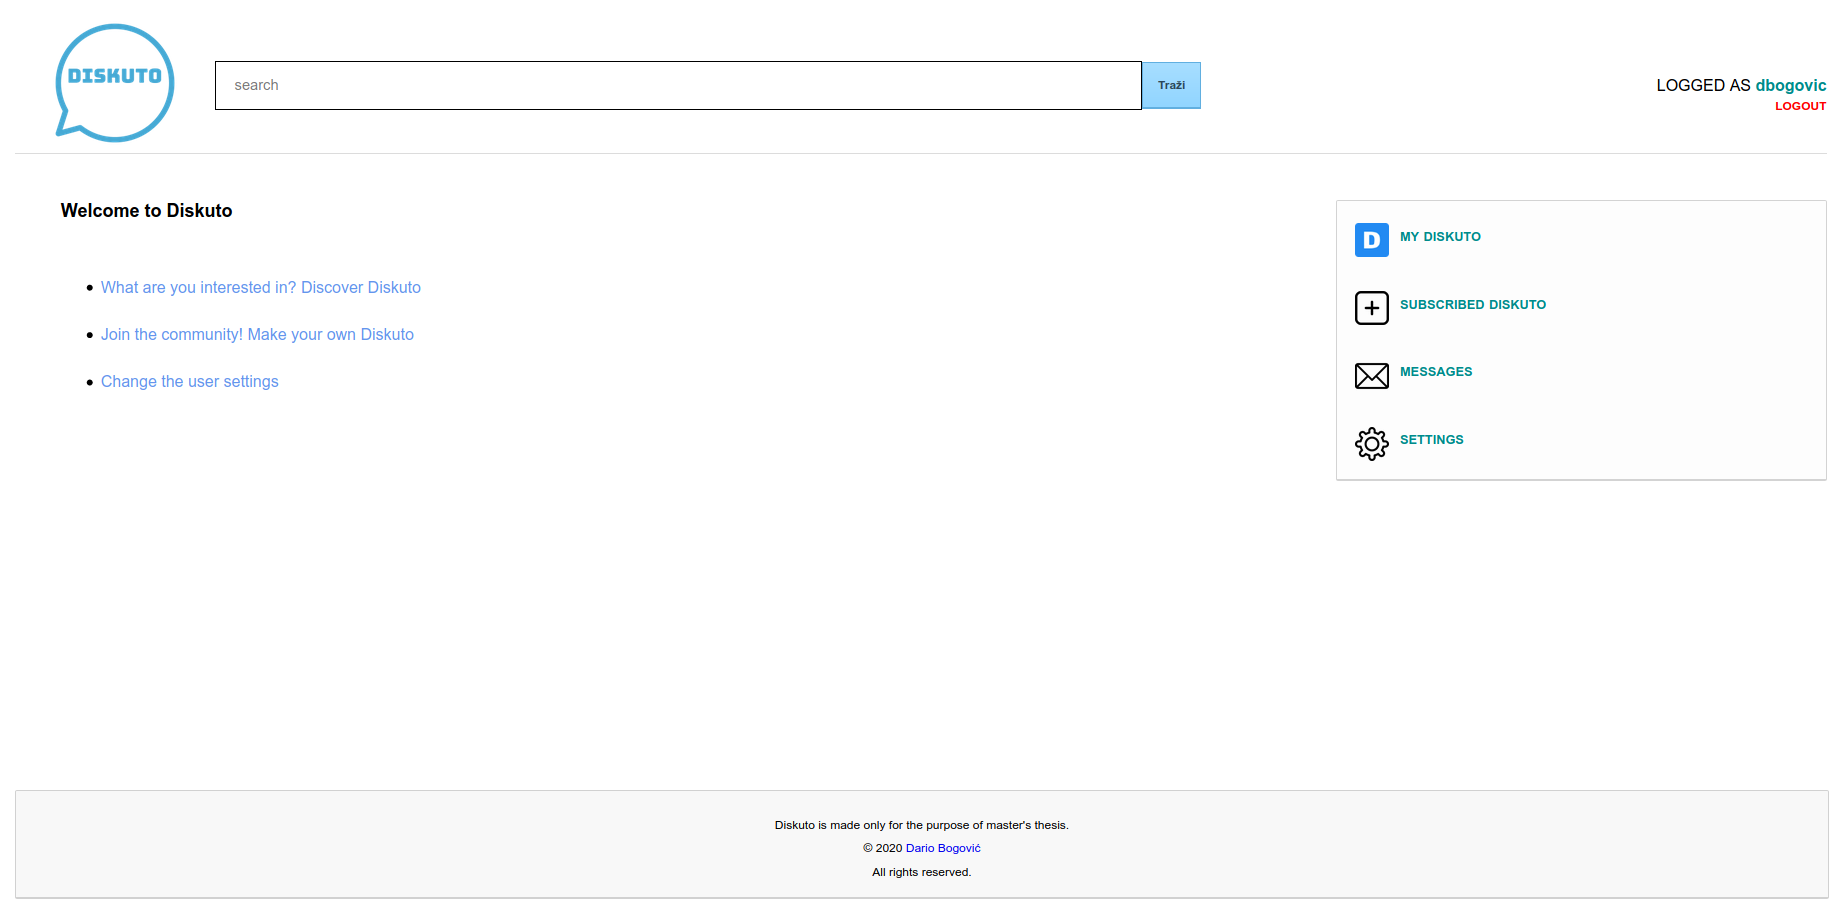
\includegraphics[width=1\textwidth]{slike/novoregistrirani-pocetna.png}
    \caption{Prikaz početne stranice za novoregistriranog korisnika}
    \label{novoregistrirani-pocetna}
\end{figure}

Potvrdom registracije, korisnika se preusmjerava na početnu stranicu koja je prikazana na slici \ref{novoregistrirani-pocetna}. Ona sadrži sve kao i početna stranica za druge korisnike, osim što na mjestu gdje bi trebali biti prikazane objave prikazuje se neke smjernice za novog korisnika. Savjetuje mu se da otkrije forume i pretplati se na njih, da ima mogućnost kreirati svoje forume i uređivati ih, te da pogleda stranicu sa postavkama gdje može urediti svoje korisničke podatke ili promijeniti jezik aplikacije.

\section{Prijava}

\begin{figure}[h!]
    \centering
    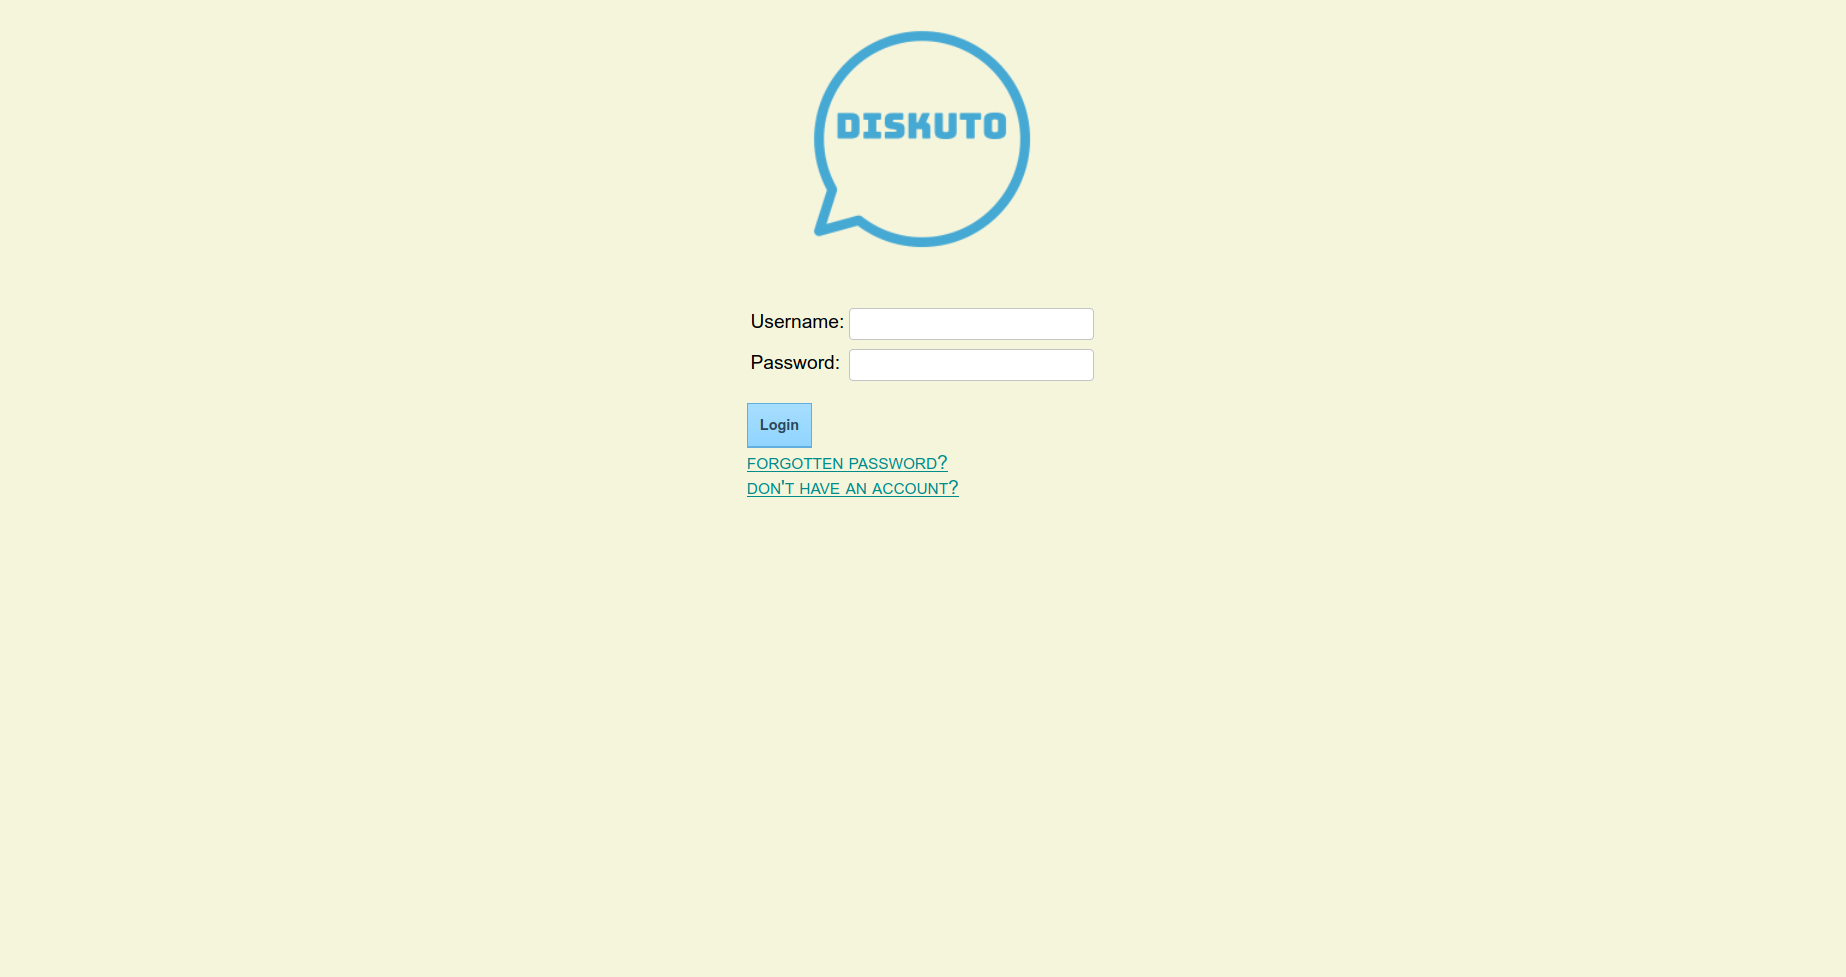
\includegraphics[width=1\textwidth]{slike/prijava.png}
    \caption{Forma za prijavu korisnika}
    \label{prijava}
\end{figure}

U zaglavlju početne stranice, odabirom na poveznicu "Login", korisnika se preusmjerava na stranicu za prijavu prikazanu na slici \ref{prijava}. Kako bi se prijavio u aplikaciju, korisnik je dužan unijeti svoje korisničko ime i lozinku. Jedino sa ispravnim korisničkim imenom i lozinkom korisnik se može prijaviti u aplikaciju, inače mu se javlja poruka o neispravno unesenim podacima. Ako korisnik nema korisnički račun, pritiskom na poveznicu "Don't have an account?" preusmjerava ga se na stranicu za registraciju. Ako je korisnik zaboravio lozinku, klikom na poveznicu "Forgotten password?" otvara mu se stranica za poništavanje lozinke.

\begin{figure}[h!]
    \centering
    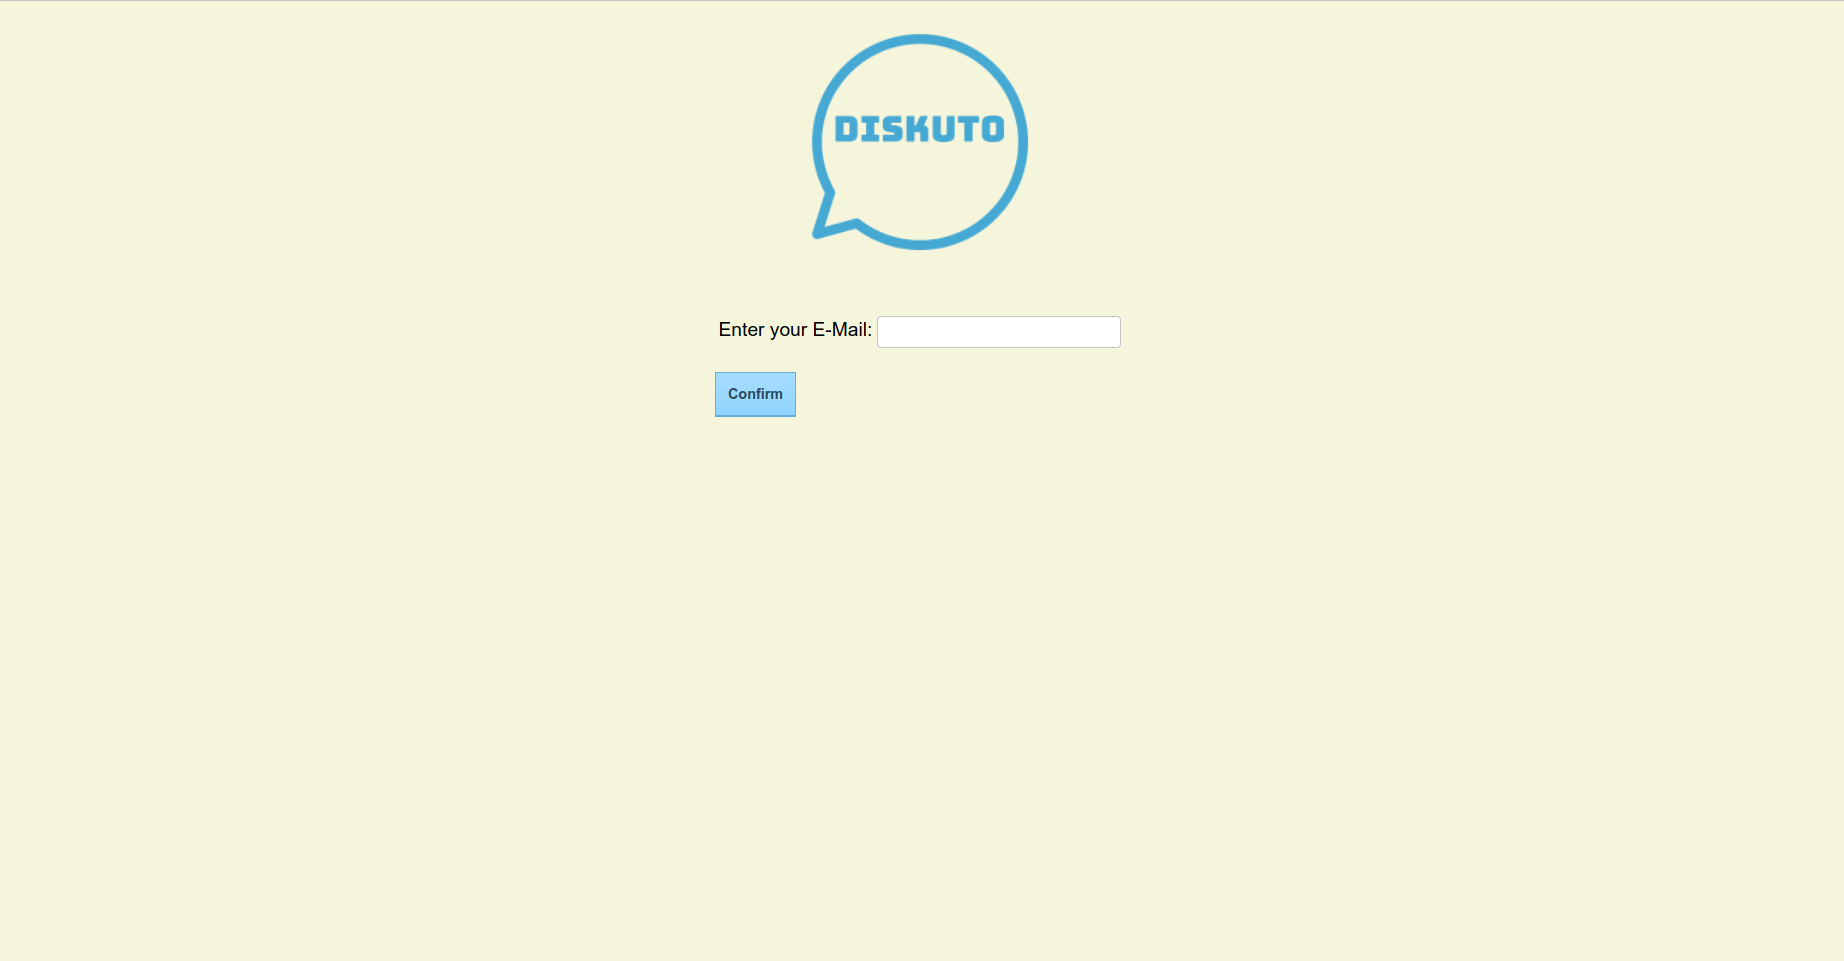
\includegraphics[width=1\textwidth]{slike/zaboravljena-lozinka.png}
    \caption{Stranica za poništavanje lozinke}
\end{figure}

Korisnik mora unijeti svoj e-mail na kojem će se poslati poveznica za kreiranje nove lozinke. Ako je e-mail nepostojeći u bazi, javit će se poruka greške. Nakon unosa pravilnog e-maila, korisniku se poništava stara lozinka i šalje mu se poruka sa uputama za kreiranje nove lozinke. U poruci će dobiti poveznicu koja ga vodi do forme za kreiranje nove lozinke. Moraju se poštivati ista pravila pri unosu lozinke kao i kod registracije (ne smije imati manje od 8 znakova i lozinka i ponovljena lozinka moraju biti jednake), u suprotnosti javit će mu se greška i korisnik neće moći obnoviti lozinku. Sve dok korisnik ne zada novu lozinku neće se moći prijaviti u aplikaciju. Obnovom lozinke korisnik se može prijaviti u aplikaciju i služiti se njome.

\section{Pronalaženje Diskuta}

Na početnoj stranici u glavnom izborniku, odabirom opcije "Pretplaćena Diskuta" (eng. "Subscribed Diskuto") korisniku se otvara stranica za pronalaženje zanimljivih foruma na koje bi se mogao pretplatiti i pratiti ih. Izgled ove stranice je prikazan na slici \ref{otkrij}.

\begin{figure}[h!]
    \centering
    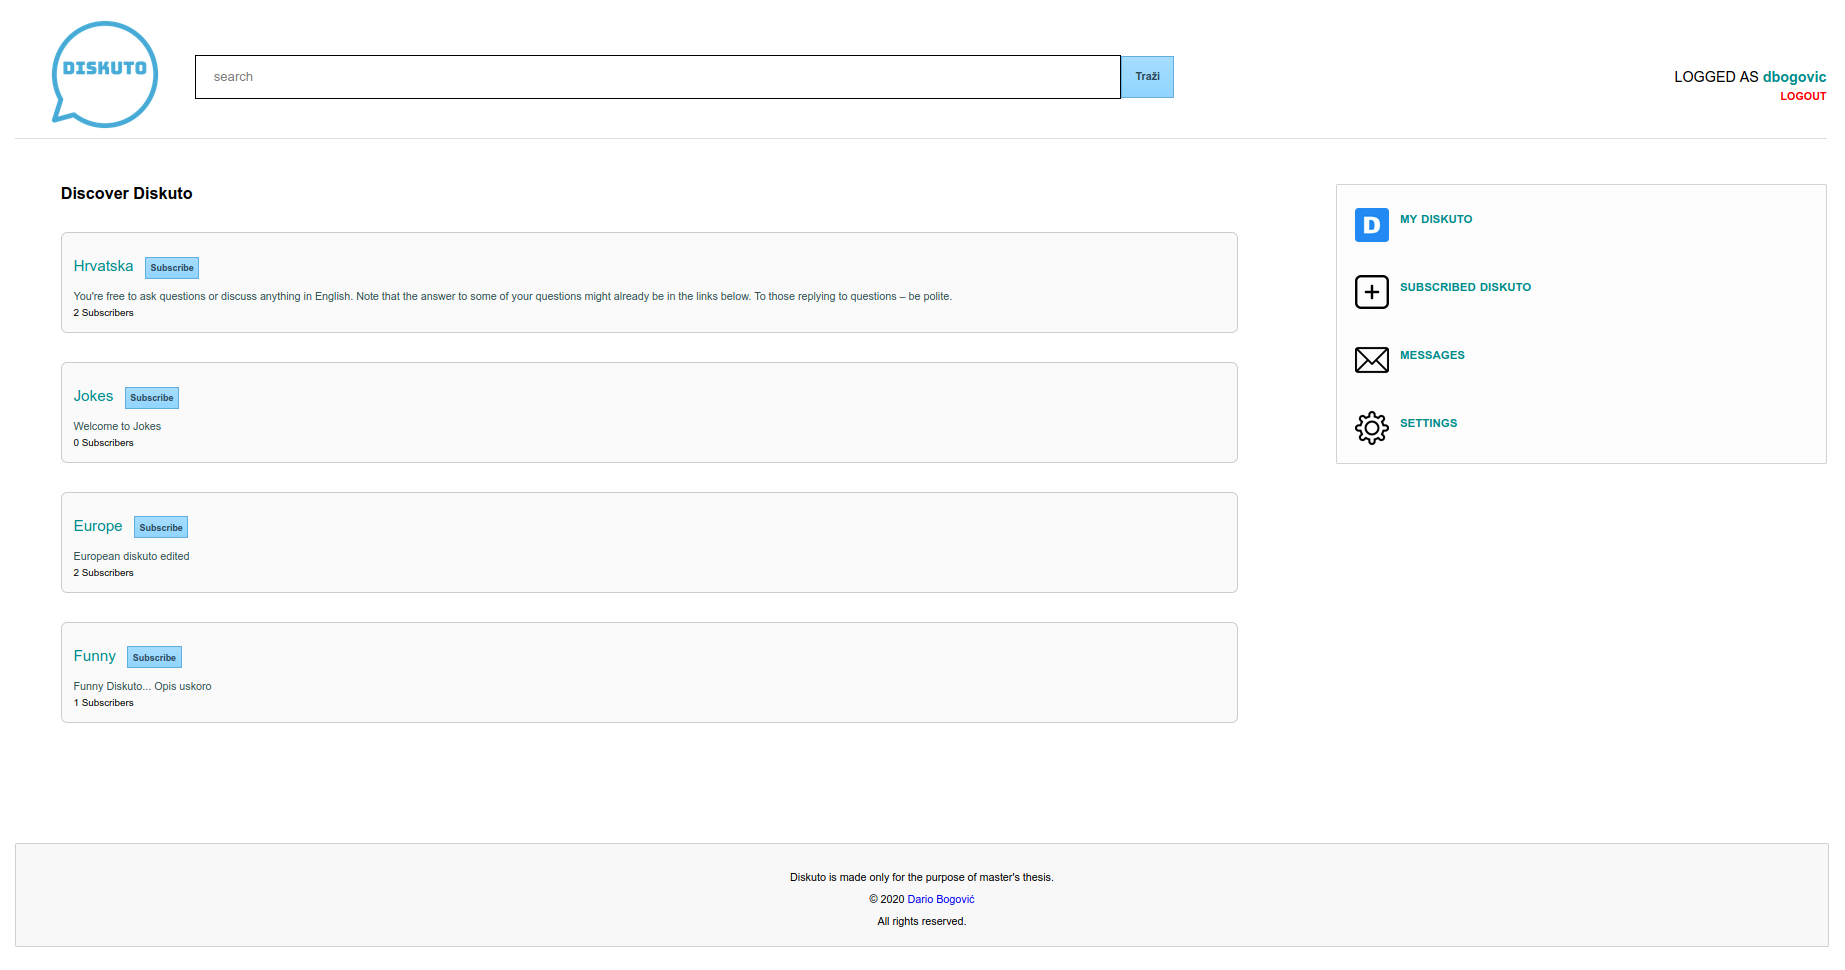
\includegraphics[width=1\textwidth]{slike/otkrij.png}
    \caption{Stranica za otkrivanje Diskuta}
    \label{otkrij}
\end{figure}

Korisniku se prikazuje popis svih foruma koji se nalaze u bazi podataka.  Za svaki pojedinačni forum je prikazan naziv, opis i broj pretplaćenih korisnika. Klikom na naziv, korisnika se preusmjerava na odabrani forum. Kraj naziva postoji jedan gumb preko kojeg je moguće pretplatiti se, odnosno ukinuti pretplatu ako već postoji pretplata na njega. Pretplatom na forum, korisnik postaje njegov član i na početnoj stranici prima najnovije objave koje su objavljene na njemu. Pretplaćeni forumi se prikazuju u glavnom izborniku odmah ispod opcije za pretragu foruma, čime korisnik može na brz i jednostavan način svojim forumima pristupiti.

\section{Kreiranje novog Diskuta}

Kako bi kreirao novi forum, korisnik se mora prebaciti na stranicu "Moja Diskuta" (eng. "My Diskuto") tako da odabere opciju u glavnom izborniku. Korisniku se tada prikazuje popis svih foruma kojih je vlasnik i na kojima je moderator. Pritiskom na gumb "Novi Diskuto" (eng. "New Diskuto"), korisniku se otvara forma za kreiranje novog foruma.

\begin{figure}[h!]
    \centering
    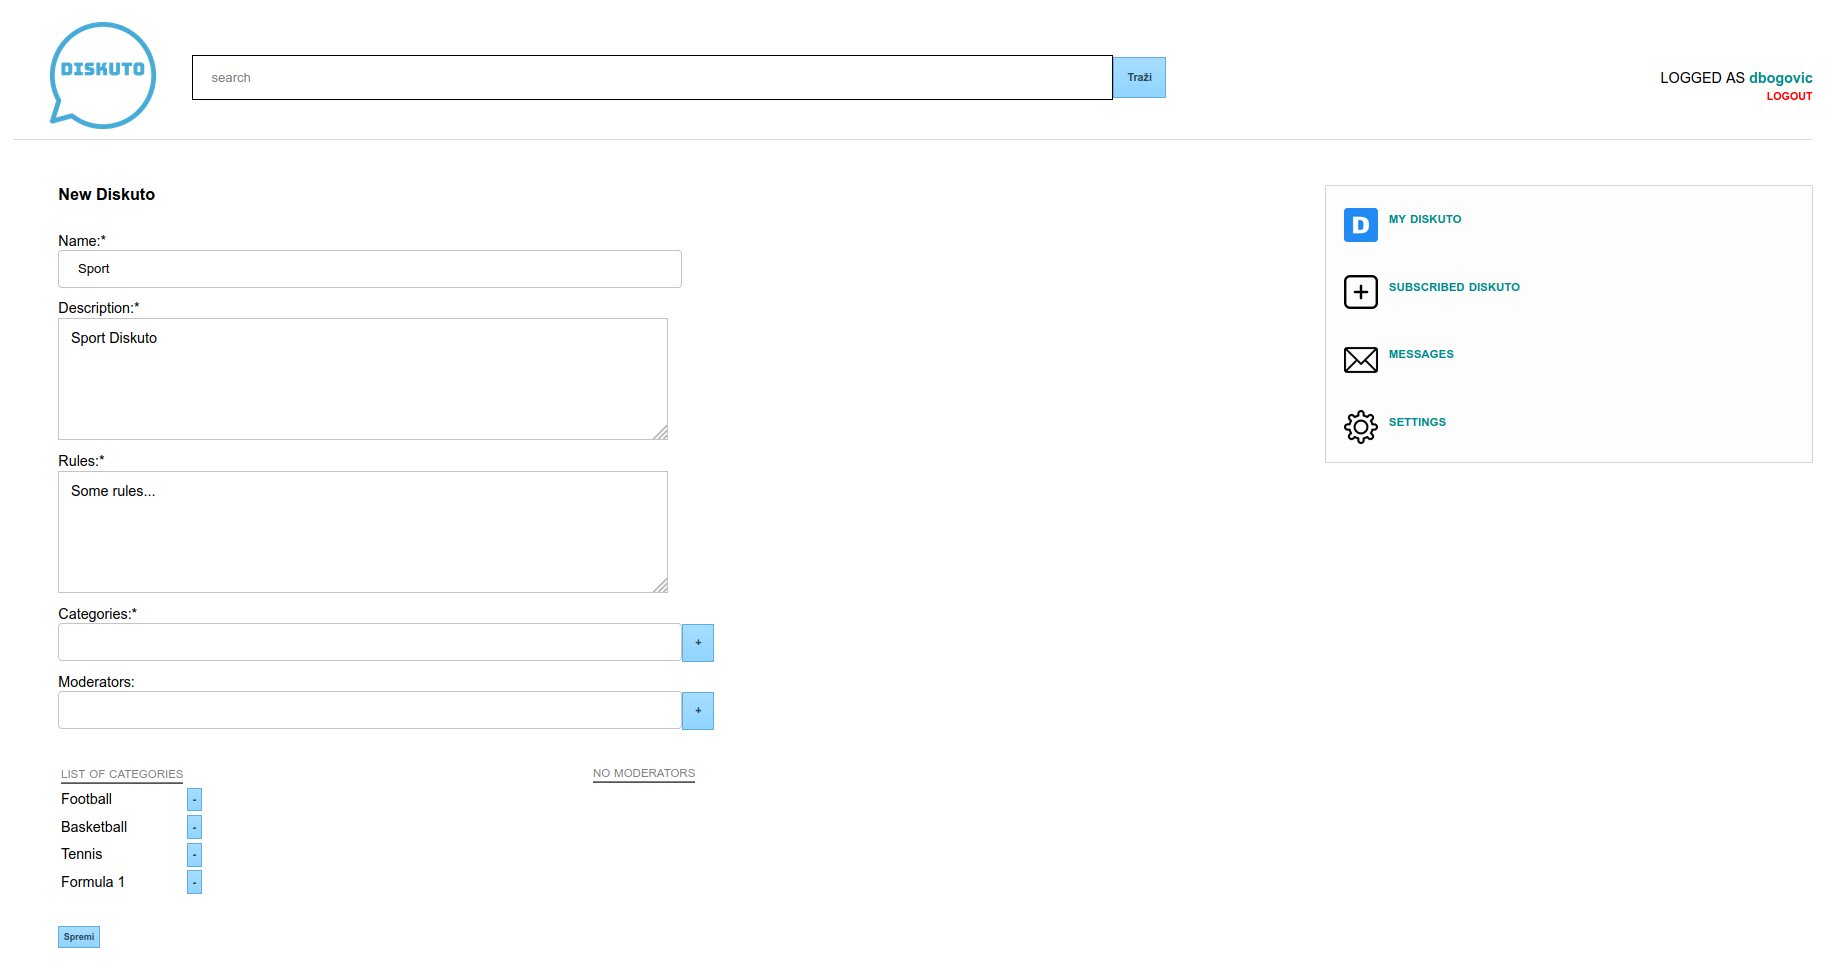
\includegraphics[width=1\textwidth]{slike/novi-forum.png}
    \caption{Forma za kreiranje novog Diskuta}
\end{figure}

Obavezno je unijeti naziv foruma, njegov opis, pravila, te barem jednu kategoriju koju će forum sadržavati. Opcionalno je moguće dodati moderatore koji će moderirati rasprave i sankcionirati eventualna kršenja pravila. Naziv foruma je konačan i njega se nakon kreiranja ne može promijeniti, dok svi drugi atributi mogu kasnije biti modificirani. Postoji ograničenje da ne smije postojati forum sa istim nazivom u bazi. U slučaju greške korisniku će se ispisati poruka, a tek kada svi podaci budu pravilno uneseni podaci se spremaju u bazu i forum postaje kreiran.

\begin{figure}[h!]
    \centering
    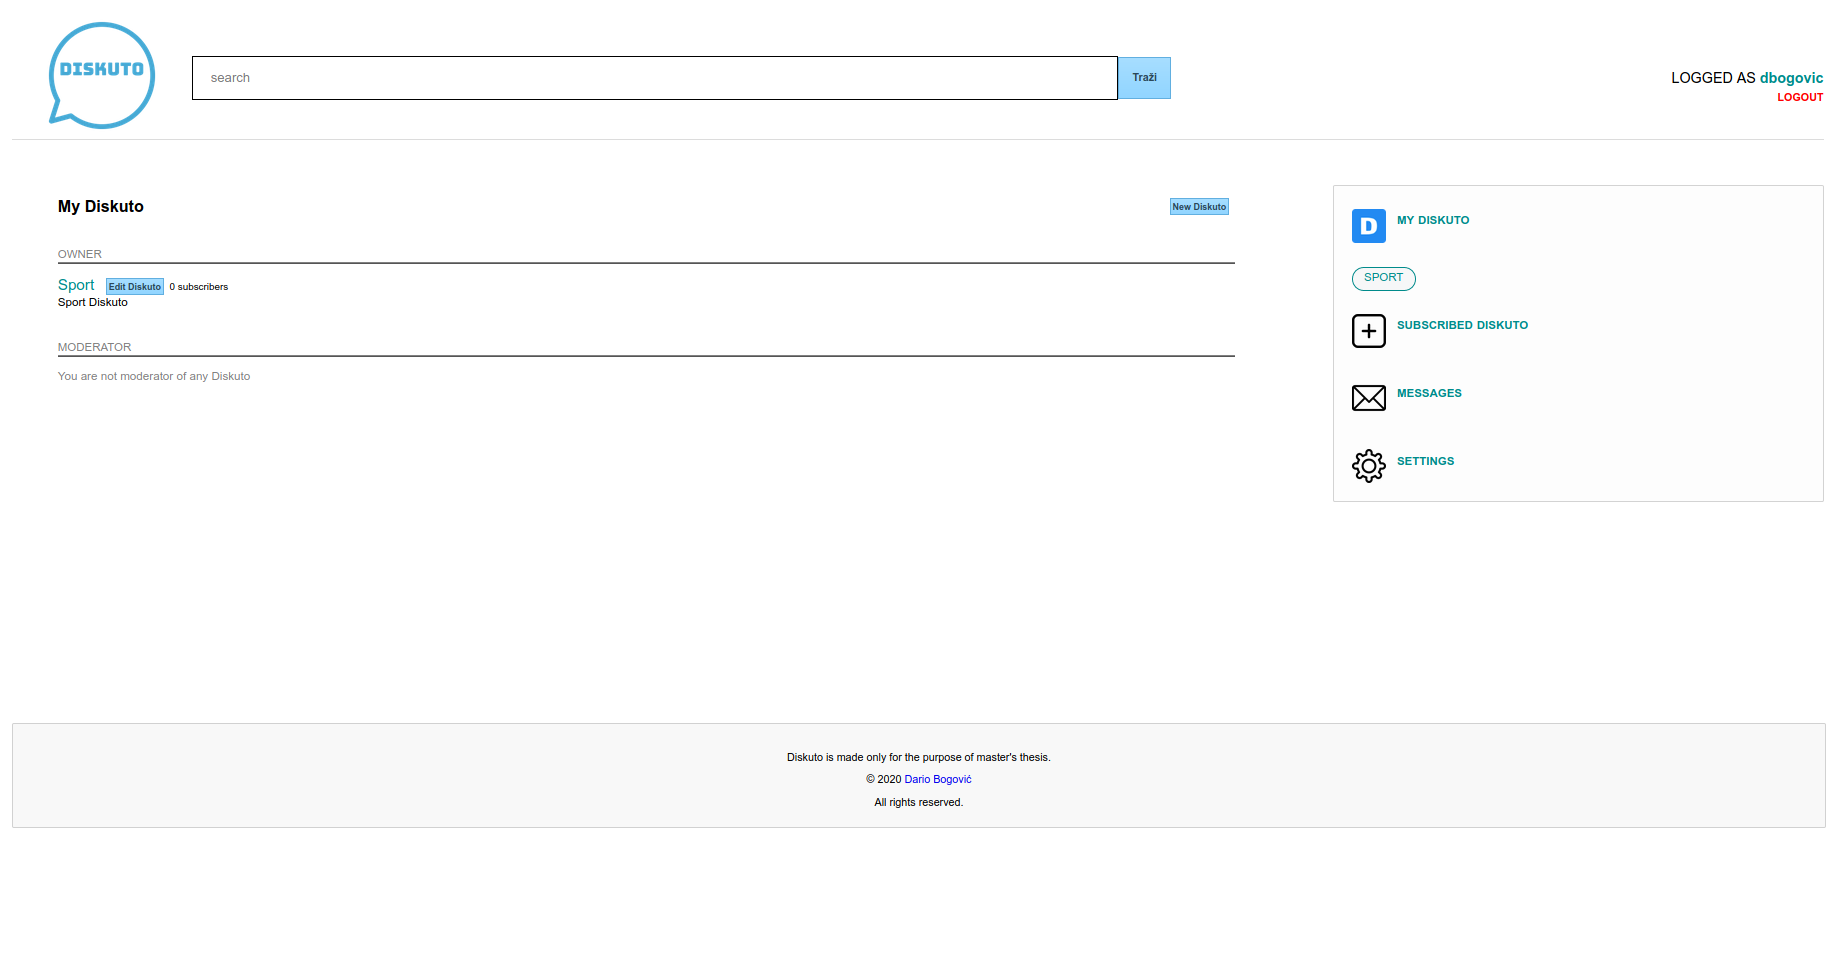
\includegraphics[width=1\textwidth]{slike/moji-forumi.png}
    \caption{Popis mojih Diskuta}
\end{figure}

Korisnika se preusmjerava na stranicu sa popisom foruma kojima je vlasnik ili moderator. Novokreirani forum se prikazuje u tablici, kao i u glavnom izborniku sa desne strane. Klikom na gumb "Uredi Diskuto" (eng. "Edit Diskuto"), korisnik može promijeniti opis i pravila foruma, brisati i dodavati kategorije, te korisnicima davati ili uklanjati ovlasti za moderatora foruma.

\section{Pregled Diskuta}

\begin{figure}[h!]
    \centering
    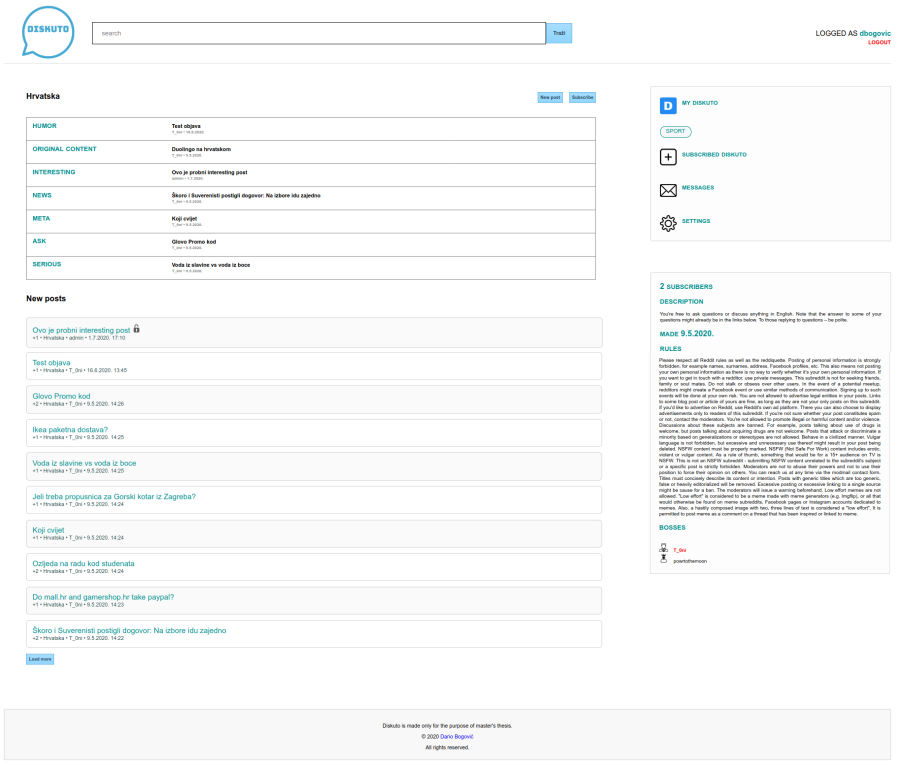
\includegraphics[width=1\textwidth]{slike/forum.png}
    \caption{Izgled stranice foruma}
    \label{forum}
\end{figure}

Na slici \ref{forum} je prikazan izgled stranice foruma za korisnika koji nije vlasnik ili moderator. Ispod glavnog izbornika aplikacije prikazan je blok sa detaljima određenog foruma: broj pretplatnika, opis, datum kreiranja, pravila foruma i poveznice na profile vlasnika i moderatora foruma.  Korisnik se može pretplatiti na forum klikom na gumb "Pretplati se" (eng. "Subscribe"), a postaviti novu objavu klikom na gumb "Nova objava" (eng. "New Post"). U glavnom dijelu aplikacije se nalazi popis svih kategorija koje forum sadrži, te sa desne strane poveznicu na najnoviju objavu na pojedinoj kategoriji. Klikom na pojedinu kategoriju otvara se popis objava sa te kategorije. Ispod elementa sa kategorijama, nalazi se popis 10 najnovijih objava na forumu i gumb za učitavanje dodatnih 10 objava. Nad svakom objavom je prikazan naslov objave odnosno poveznica nad svaku objavu, karma (odnos pluseva i minusa) koju ima, forum na kojem je objavljena, poveznica na profil vlasnika objave i datum i vrijeme kreiranja objave.

\section{Kreiranje nove objave}

\begin{figure}[h!]
    \centering
    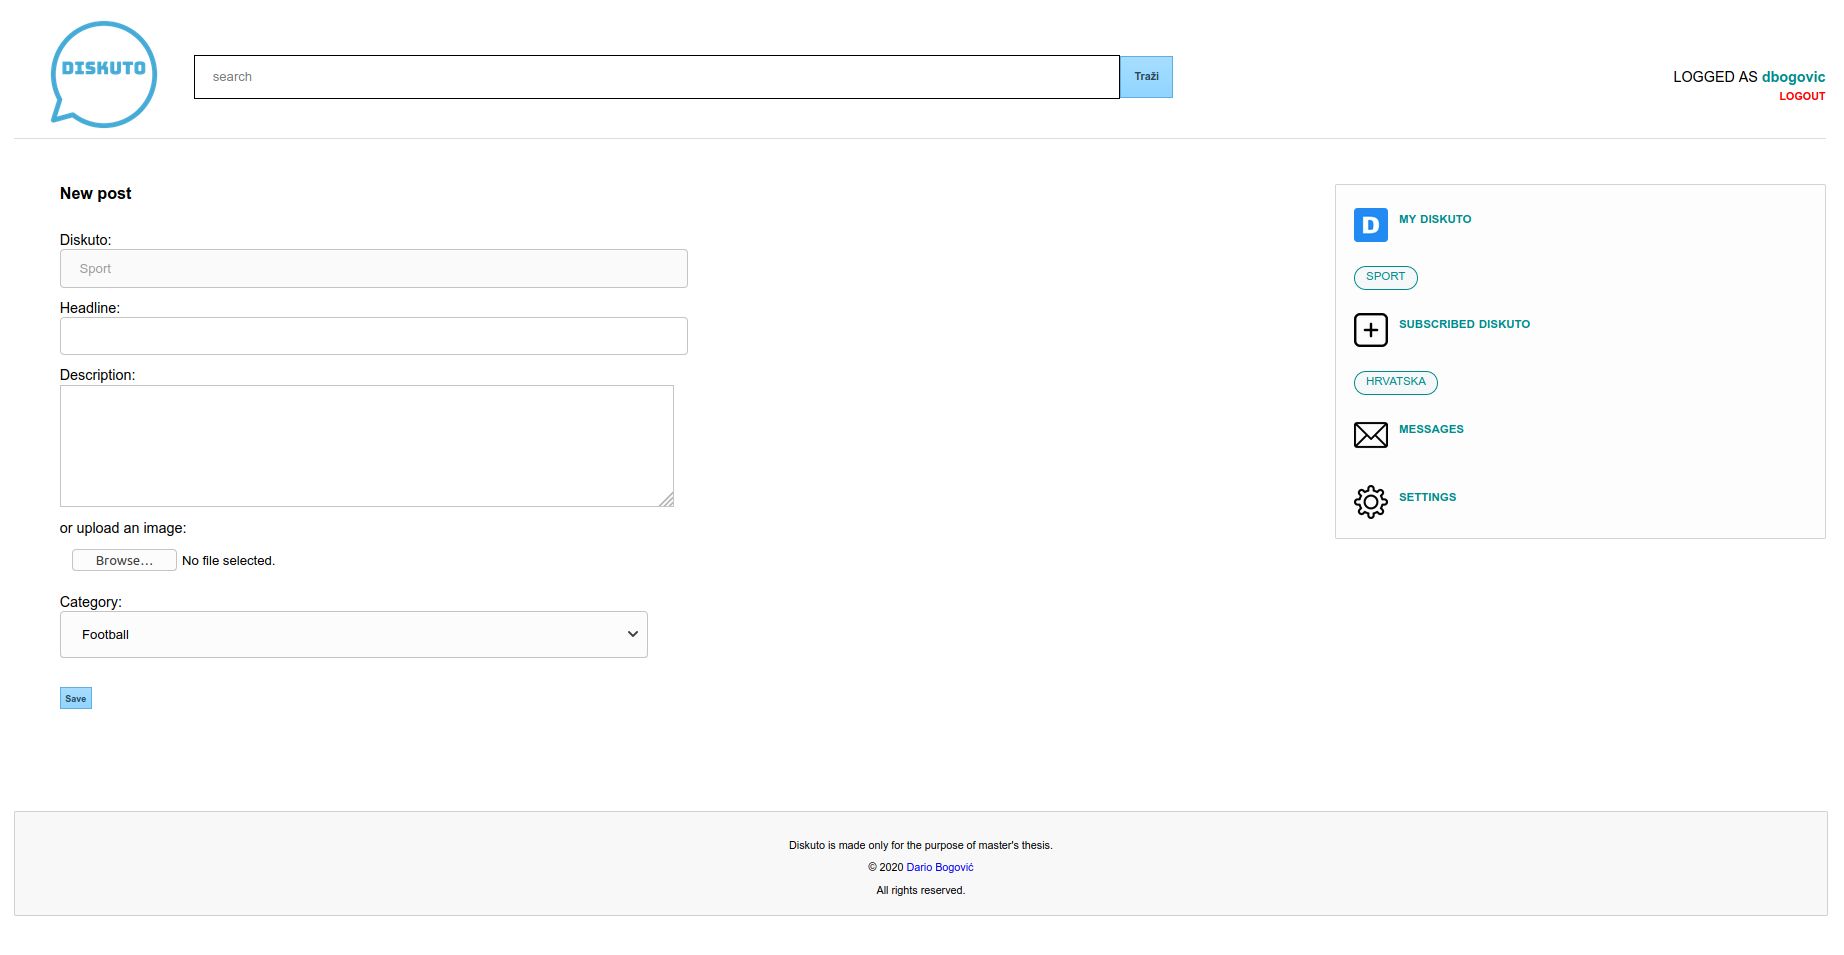
\includegraphics[width=1\textwidth]{slike/nova-objava.png}
    \caption{Forma za kreiranje nove objave}
    \label{nova-objava}
\end{figure}

Klikom na gumb za kreiranje nove objave nad pojedinim forumom, korisnika se preusmjerava na formu za kreiranje objave (slika \ref{nova-objava}). Prikazan je forum nad kojem se kreira nova objava, a korisnik mora unijeti naslov i dodatno opisati svoju objavu ili učitati sliku. Obavezno je odabrati i kategoriju na koju želi da se objava spremi. Slika koja se unosi mora biti u slikovnom formatu, a ako nije ili ako korisnik je nešto zaboravio unijeti prikazuje mu se poruka greške. Tek kada je sve u redu objava se sprema u bazu i postaje vidljiva na forumu.

\begin{figure}[h!]
    \centering
    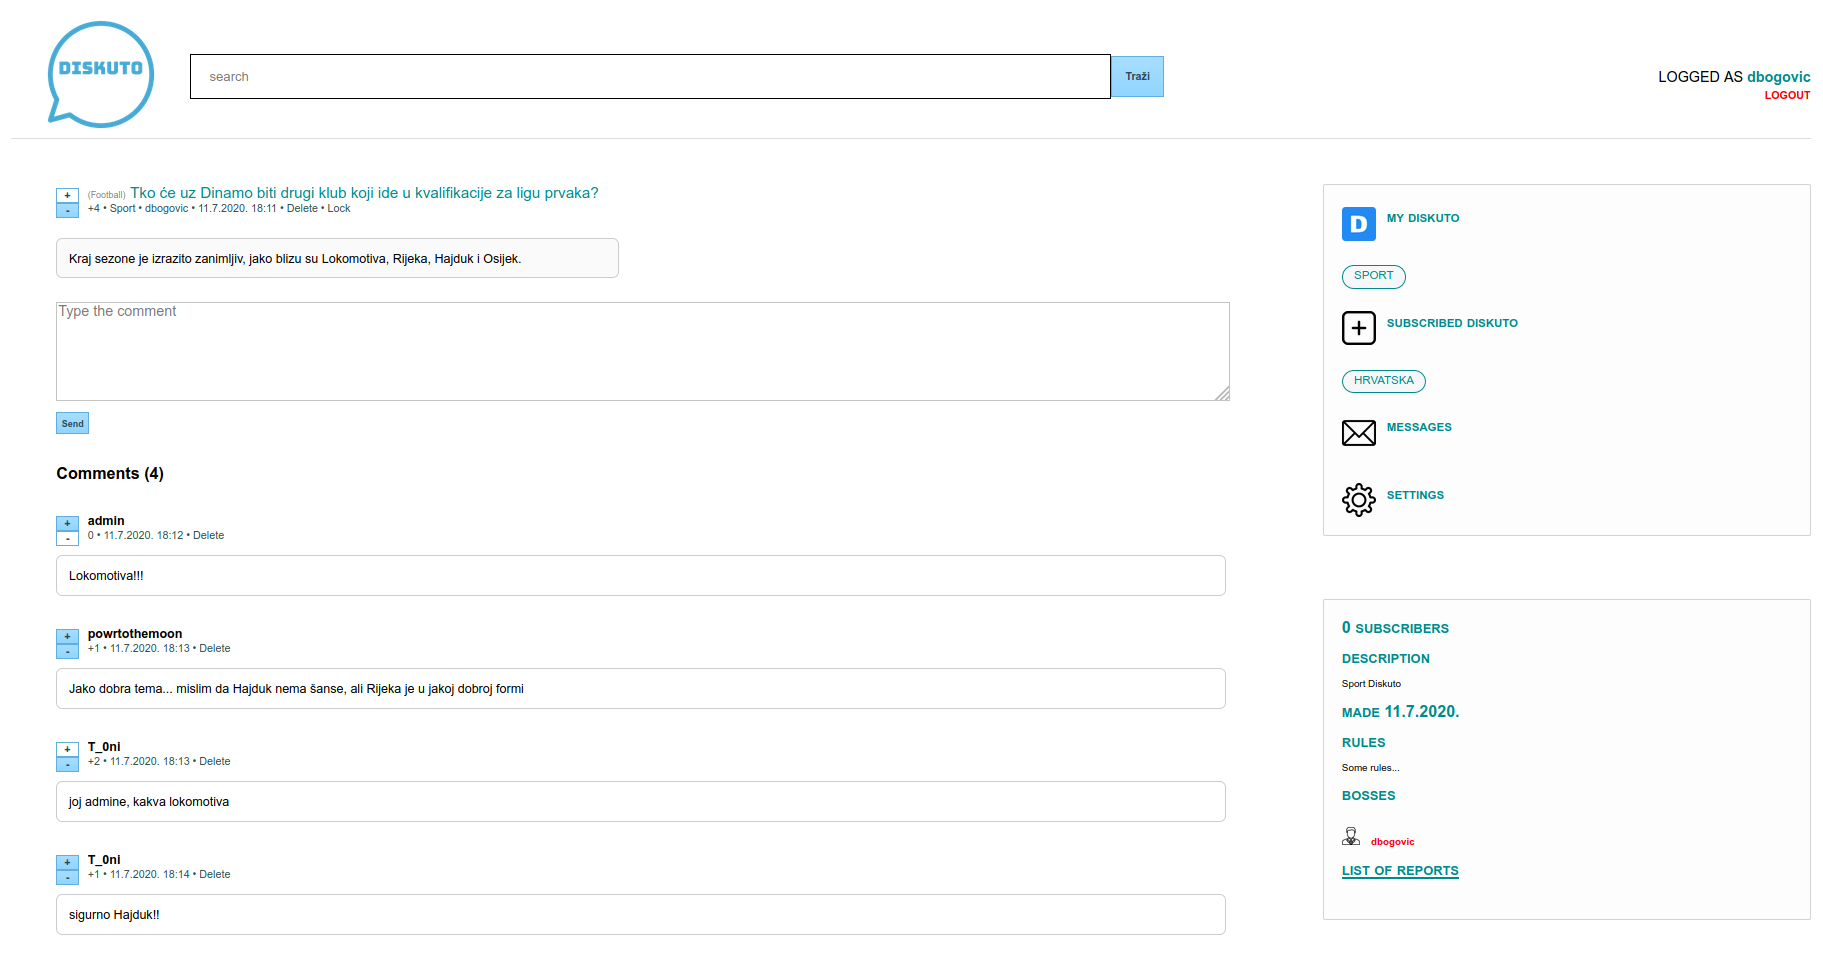
\includegraphics[width=1\textwidth]{slike/objava.png}
    \caption{Izgled objave}
    \label{objava}
\end{figure}

Izgled objave je vidljiv na slici \ref{objava}. Prikazan je naslov objave, poveznica do stranice kategorija foruma na kojem je ona objavljena, karma (odnos pluseva i minusa) koju ima, forum na kojem je objavljena, autor i vrijeme kreiranja objave. Sa lijeve strane se nalazi gumb za označavanje objave sa "+" čime se povećava karma objave i karma autora, odnosno sa "-" čime se smanjuje karma objave i karma autora. Prema zadanome autor objave automatski sam sebi zadaje "+", ali naknadno može si maknuti "+" ili si dodijeliti "-". U svakom trenutku autor objave može obrisati svoju objavu. Ako drugi korisnici foruma smatraju da objava krši pravila foruma, mogu ju prijaviti moderatorima. Ispod naslova objave slijedi tekstualni opis ili slika objave, ovisno o tome što je autor stavio kao opis. Ispod opisa se nalazi tekstualno polje za unos komentara koji se sprema u bazu pritiskom na gumb ispod njega. Zatim se nalazi element sa komentarima koji ispisuje broj ukupnih komentara i sadržaj komentara. Nad svakim komentarom se ispisuje autor objave i poveznica do njegovog profila, karma (odnos pluseva/minusa), datum i vrijeme kada je komentar postavljen, tekst komentara i gumbi sa označavanjem komentara kao "+" čime se povećava karma komentara i njegovog autora, odnosno kao "-" čime se smanjuje karma komentara i njegovog autora. Prema zadanome autor komentara automatski sam sebi zadaje "+", ali naknadno može si maknuti "+" ili si dodijeliti "-". Ispod se nalazi sami tekst komentara. U svakom trenutku autor komentara može obrisati svoj komentar. Ako drugi korisnici foruma smatraju da komentar krši pravila foruma, mogu ga prijaviti moderatorima.

\section{Ovlasti moderatora nad pojedinim Diskutom}

Kao što je već opisano u poglavlju kod kreiranja foruma, moderatori imaju naprednije ovlasti nad forumom od običnih korisnika. Imaju iste ovlasti kao i vlasnik, a oni se dodaju i brišu na stranici za uređivanje i brisanje foruma. Razlika u odnosu na vlasnika je jedino ta što je vlasnik "doživotni moderator", odnosno on ima trajne i neopozive ovlasti nad forumom. Moderatori mogu obrisati bilo koju objavu ili komentar za koji smatraju da je neprimjeren, za razliku od običnih korisnika koji jedino mogu obrisati svoju objavu/komentar. Moderatori mogu zaključati objavu i tako onemogućiti komentiranje na njoj. U svakom trenutku objava se može otključati i tako omogućiti korisnicima da nastave komentirati. Zaključane objave imaju kraj svog naslova ikonu lokota, čime se razlikuju od drugih otključanih objava. Drugi korisnici mogu moderatorima prijaviti objave ili komentare za koje smatraju da su neprimjerene. U elementu opisa foruma, moderatori klikom na poveznicu "Popis prijava" (eng. "List of reports") mogu otvoriti stranicu sa popisom svih prijavljenih objava/komentara na njihovom forumu.

\begin{figure}[h!]
    \centering
    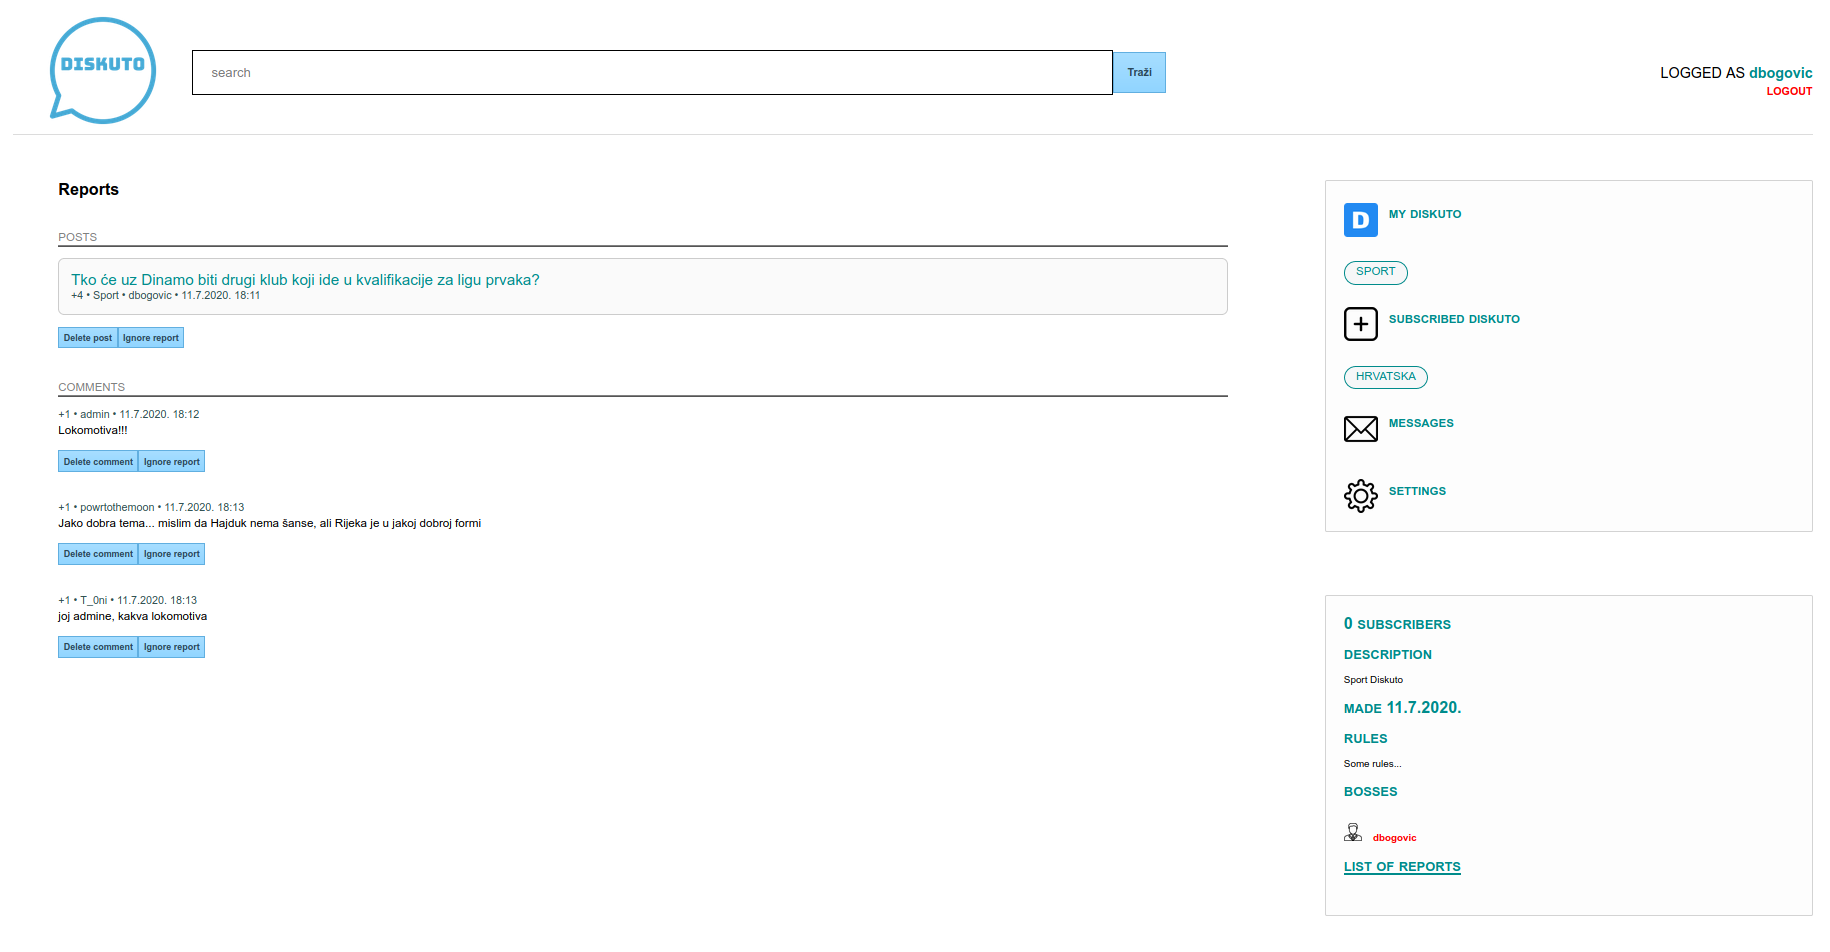
\includegraphics[width=1\textwidth]{slike/prijave.png}
    \caption{Popis prijavljenih objava/komentara}
\end{figure}

Moderatori mogu odlučiti obrisati objavu/komentar ako smatraju da krši pravila foruma ili zanemariti prijavu ako smatraju da je sve u redu.

\section{Profil korisnika}

\begin{figure}[h!]
    \centering
    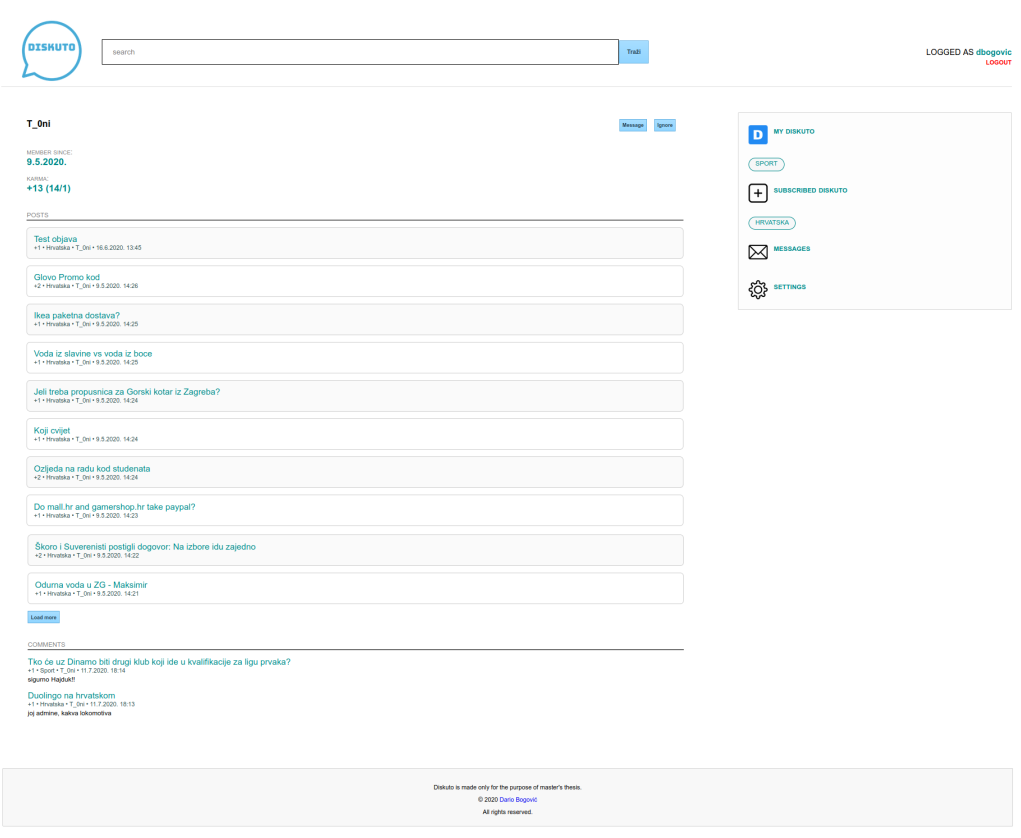
\includegraphics[width=1\textwidth]{slike/profil.png}
    \caption{Profil korisnika}
    \label{profil}
\end{figure}

Bilo gdje na stranici kada se klikne na korisničko ime pojedinog korisnika, preusmjerava se na stranicu njegovog profila kao na slici \ref{profil}. U glavnom dijelu stranice vidljivo je korisničko ime i gumbi za slanje poruke korisniku i za ignoriranje korisnika. Kada se klikne gumb za slanje poruke, korisnika se preusmjerava na stranicu sa porukama na kojoj može vidjeti prethodnu komunikaciju sa odabranim korisnikom (ako je bilo) i ima mogućnost poslati mu poruku. Naravno to je moguće ako korisnik nije drugog korisnika blokirao (ili obratno). Klikom na gumb za ignoriranje korisnik više neće vidjeti objave i komentare odabranog korisnika, kao ni primati i slati privatne poruke od njega. Deblokirati ga se može u postavkama korisničkog računa ili ako korisnik ponovno ode na njegov profil i klikne gumb za deblokiranje. Ispod naziva korisničkog imena i gumbova, mogu se vidjeti detalji o odabranom korisniku poput datuma kada je kreiran korisnički račun i ukupne karme (razlika između pluseva i minusa na svim objavama i komentarima). Ispod ovog elementa, navedene su sve objave i svi komentari pojedinog korisnika. Radi boljih performansi stranice navedeno je samo 10 njih, a klikom na gumb za učitavanje može se učitati dodatnih 10 objava/komentara. Kod objava vidljiv je naslov objave čijim odabirom se preusmjerava na samu objavu, te detalji o objavi: karma, datum kreiranja i forum na kojem je objavljen. Kod komentara vidljiv je naslov objave na kojoj je komentar objavljen i čijim odabirom se preusmjerava na samu objavu, detalji poput karme, datuma kreiranja, foruma na kojem je objavljen, te na kraju sami tekst komentara.

\section{Poruke}

Osim što korisnici mogu javno komunicirati, oni mogu slati jedni drugima i privatne poruke. Korisnik inicira razgovor sa drugim korisnikom odabirom gumba za slanje poruka na njegovom privatnom profilu. Tada se korisnika preusmjerava na stranicu sa porukama kojoj se može pristupiti i sa glavnog izbornika odabirom opcije "Poruke" (eng. "Messages"). 

\begin{figure}[h!]
    \centering
    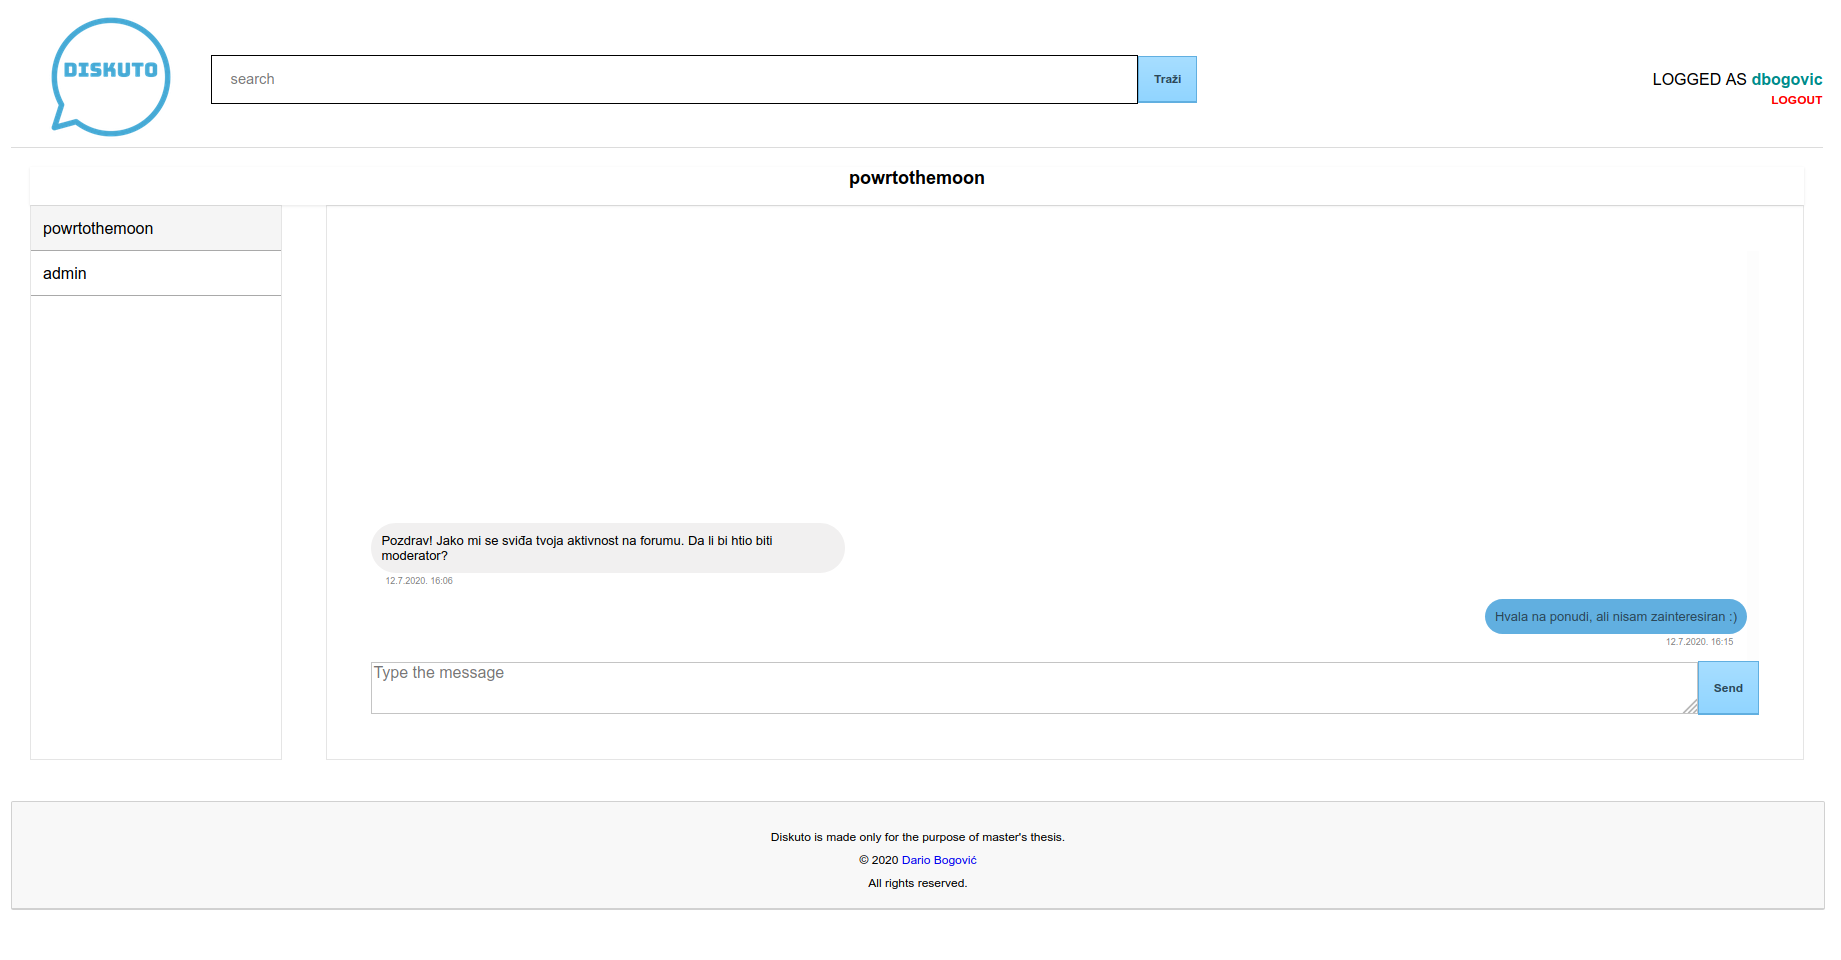
\includegraphics[width=1\textwidth]{slike/poruke.png}
    \caption{Poruke}
    \label{poruke}
\end{figure}

Prikaz stranice za slanje privatnih poruka je vidljiv na slici \ref{poruke}. Između zaglavlja i podnožja stranice nalazi se glavni dio stranice koji se sastoji od: korisničkog imena korisnika sa kojim je trenutno aktivna komunikacija i poveznica na njegov profil, s lijeve strane popis svih korisnika sa kojima je korisnik komunicirao u prošlosti i poveznica na njihovu stranicu komunikacije, te u glavnom dijelu se nalaze same poruke koje su korisnici međusobno razmijenili. Poruke koje je korisnik primio su poravnate sa lijeve strane i imaju crnu boju teksta na sivoj pozadini. Poruke koje je korisnik poslao su poravnate sa desne strane i imaju tamnoplavu boju teksta na plavoj pozadini. Ispod svake poruke nalazi se točan datum i vrijeme kada je poruka poslana ili primljena. Ispod elementa sa porukama nalazi se tekstualni element za slanje poruke. Poruku je jedino moguće poslati ako se korisnici ne ignoriraju, odnosno ako jedan nije stavio drugoga na listu ignoriranja. Kada pošiljatelj pošalje poruku, primatelja se obaviještava na način da u glavnom izborniku aplikacije mu se prikaže da ima nepročitanu poruku i ispod mu se prikaže na poveznicu razgovora sa korisnikom od kojeg je primio poruku. Sve dok primatelj poruku ne pročita, ta će mu obavijest biti prikazana u glavnom izborniku.

\section{Pretraga}

Tijekom većine vremena služenja sa aplikacijom se u zaglavlju nalazi traka za pretragu foruma. Registrirani korisnici mogu pretražiti po ključnoj riječi sve forume, korisnike i objave na forumima. Ako je ključna riječ sadržana u nazivu foruma kao rezultat pretrage će se vratiti naziv i poveznica na forum, opis, broj pretplatnika i gumb za pretplatu na navedeni forum. Ako je ključna riječ sadržana u korisničkom imenu korisnika kao rezultat pretrage će se vratiti korisničko ime i poveznica na profil, te gumb za slanje privatne poruke korisniku. Ako je ključna riječ sadržana u naslovu objave na nekom forumu kao rezultat pretrage će se vratiti naslov i poveznica na objavu, te podaci o objavi (karma, forum na kojem je objavljena, autor objave, datum i vrijeme objave).

\begin{figure}[h!]
    \centering
    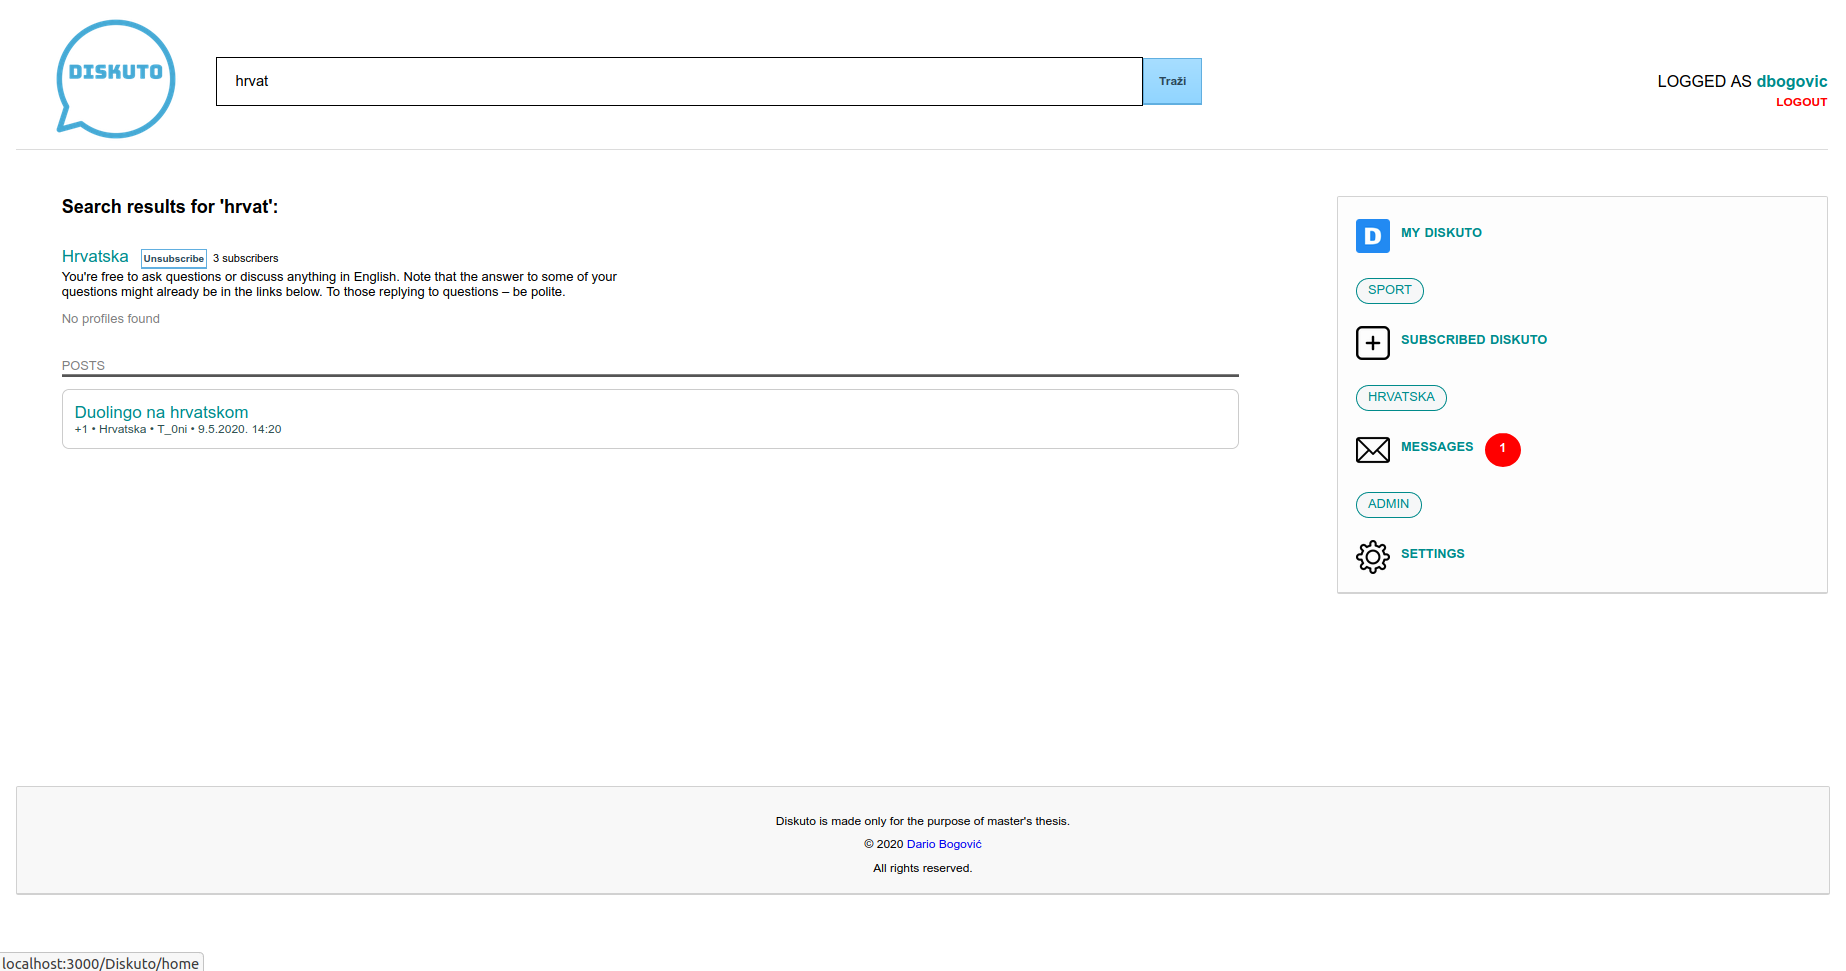
\includegraphics[width=1\textwidth]{slike/pretraga.png}
    \caption{Izgled stranice za pretragu}
    \label{pretraga}
\end{figure}

Na slici \ref{pretraga} je prikazan primjer izgleda stranice za pretragu ako je unesena ključna riječ "hrvat". Vidljivo je kako je aplikacija vratila kao rezultat pretrage jedan forum pod nazivom "Hrvatska", niti jedan profil sa korisničkim imenom koji sadrži tu ključnu riječ, te jednu objavu koja u sebi sadrži ključnu riječ "hrvat". Ako aplikacija vrati forum kao rezultat pretrage, ona će ispisati naziv foruma koja je poveznica na stranicu foruma, gumb za pretplatu/poništenje pretplate i detalje o forumu poput broja pretplaćenih korisnika i opis. Ako aplikacija vrati korisnika kao rezultat pretrage, ona će ispisati korisničko ime koje je ujedno i poveznica na profil, te gumb čijim klikom se preusmjerava na slanje privatne poruke. Ako aplikacija vrati objavu kao rezultat pretrage, ispisat će se puni naslov objave koja je i poveznica na samu objavu, te detalji o objavi poput karme (razlika pluseva/minusa), poveznica na forum gdje je objava objavljena, poveznica na profil autora objave i datum i vrijeme kada je objava objavljena. Ako aplikacija ne vrati niti jedan forum, korisnika ili objavu ispisat će se obavijest o neuspjehu.

\section{Postavke}

\begin{figure}[h!]
    \centering
    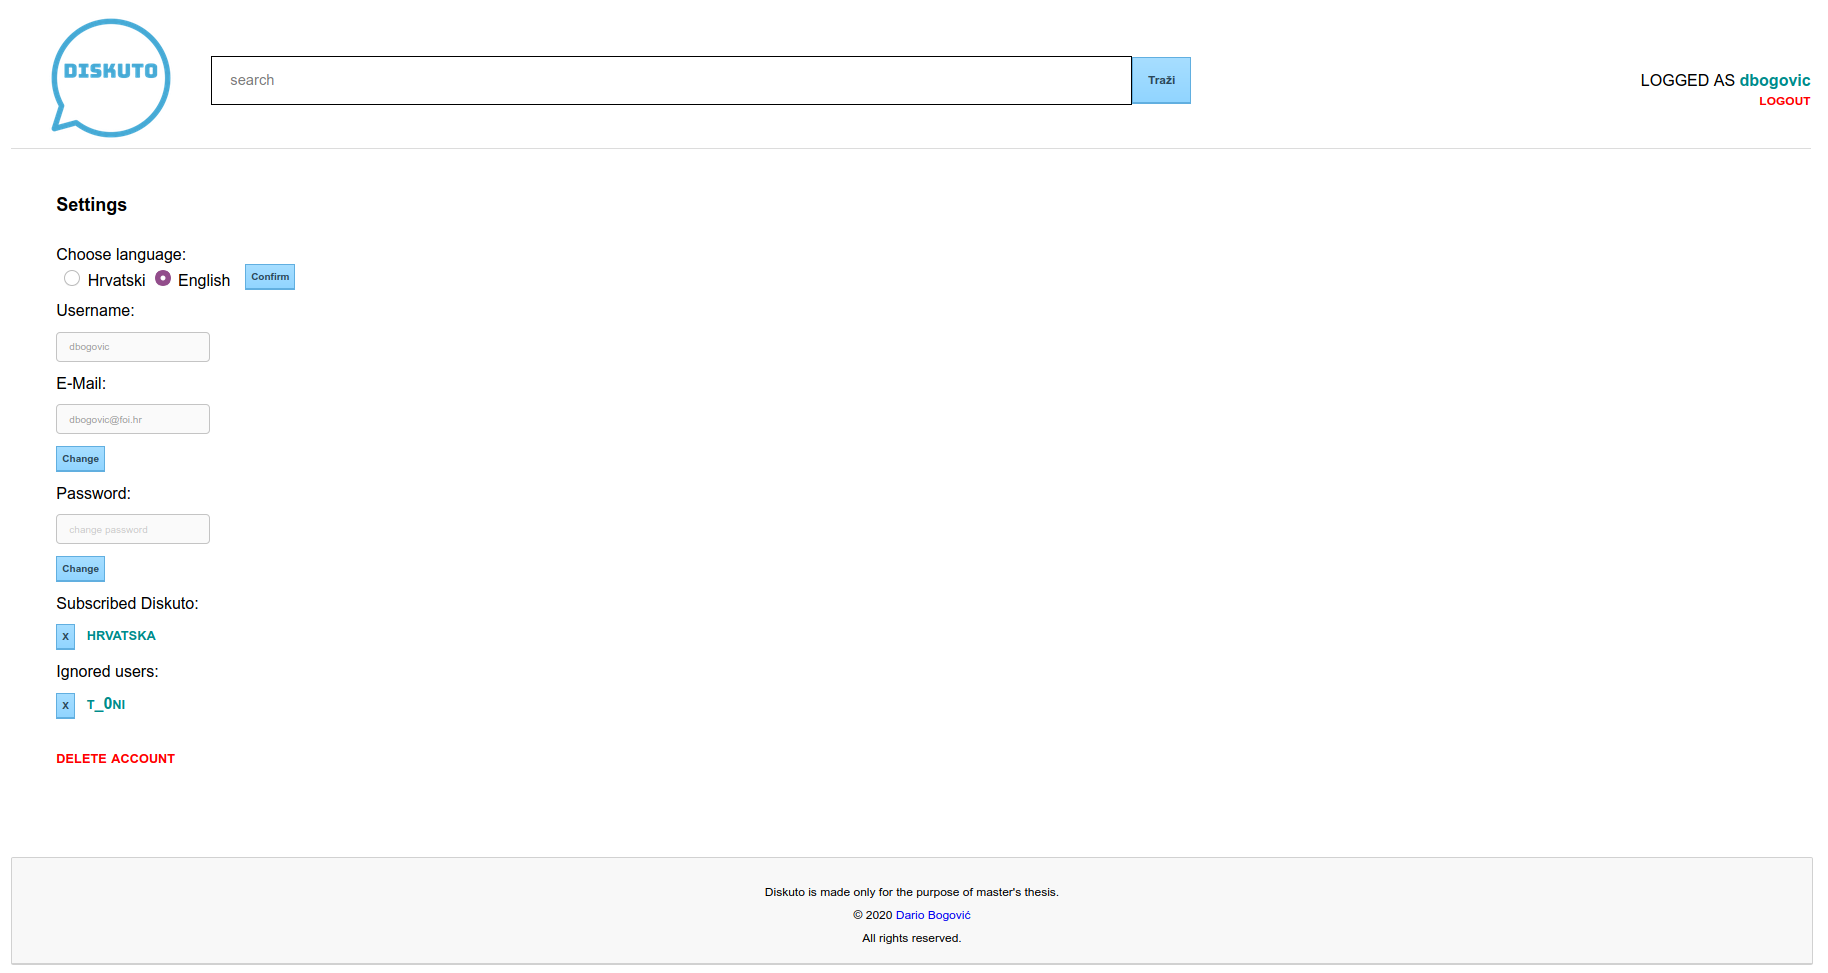
\includegraphics[width=1\textwidth]{slike/postavke.png}
    \caption{Korisničke postavke}
\end{figure}

Korisničkim postavkama se može pristupiti odabirom opcije "Postavke" (eng. "Settings") u glavnom izborniku aplikacije. Korisnik može promijeniti jezik aplikacije, a na raspolaganju su mu dva jezika: engleski i hrvatski. Klikom na gumb za promjenu spremaju se postavke i u bazi, pa kada se korisnik ponovno prijavi prikazati će mu se željeni jezik kojeg je promijenio u postavkama. Korisničko ime je nepromijenjivo, te ga se nakon registracije ne može mijenjati. Korisnik može promijeniti e-mail tako da nakon što klikne gumb za promjenu umjesto sadašnjeg unese novi e-mail. Ako unese krivi format, aplikacija mu neće dozvoliti promijenu i ispisat će se greška. Korisnik može promijeniti i svoju lozinku tako da nakon što klikne gumb za promjenu unese novu lozinku. I dalje stoji pravilo da lozinka ne smije biti preslaba, odnosno ne smije imati manje od osam znakova. Ako je lozinka preslaba, aplikacija mu neće dozvoliti promijenu lozinke i ispisat će se greška. Korisnik također može vidjeti na koje forume je trenutno pretplaćen, te klikom na gumb "X" koji stoji pokraj poveznice na forum može ukloniti pretplatu. Korisnik može vidjeti i koje je korisnike blokirao, te klikom na gumb "X" koji stoji pokraj poveznice na njegov profil može ga deblokirati. Klikom na opciju "Obriši račun" (eng. "Delete account") korisnik može trajno obrisati svoj račun. Za potvrdu je potrebno unijeti trenutnu lozinku. Ako je lozinka pogrešna ispisat će se greška, a ako unese dobru lozinku i potvrdi je račun se trajno briše i prikazuje mu se poruka kao na slici:

\begin{figure}[h!]
    \centering
    
\includegraphics[width=1\textwidth]{slike/deaktivacija.png}
    \caption{Poruka o deaktiviranom računu}
\end{figure}

\chapter{Zaključak}

\printbibliography[title=Popis literature]
\addcontentsline{toc}{chapter}{Popis literature}

\listoffigures
\addcontentsline{toc}{chapter}{Popis slika}

\lstlistoflistings
\addcontentsline{toc}{chapter}{Popis programskih isječaka}

\end{document}
